\documentclass[usenames,dvipsnames]{beamer}
\usepackage[utf8]{inputenc} % allow utf-8 input
\usepackage[T1]{fontenc}    % use 8-bit T1 fonts
\usepackage{hyperref}       % hyperlinks
\usepackage{url}            % simple URL typesetting
\usepackage{booktabs}       % professional-quality tables
\usepackage{amsfonts}       % blackboard math symbols
\usepackage{nicefrac}       % compact symbols for 1/2, etc.
\usepackage{microtype}      % microtypography
\usepackage{amsmath}
\usepackage{mathtools}
\usepackage{xcolor}
\usepackage{tikz}
\usetikzlibrary{calc}
\usetikzlibrary{bayesnet}
\usetikzlibrary{arrows}
\usepackage{color}
\usepackage{array}
\usepackage{dsfont}
\usepackage{multirow, graphicx}
 \usepackage{float}
\newcolumntype{C}[1]{>{\centering\arraybackslash}p{#1}}
\newcolumntype{R}[1]{>{\raggedleft\arraybackslash}p{#1}}
\newcolumntype{L}[1]{>{\raggedright\arraybackslash}p{#1}}
\usepackage{caption}
\usepackage{subfig}
\usepackage{pifont}
\usepackage{algorithm,algorithmic}
% \floatname{algorithm}{Procedure}
\renewcommand{\algorithmicrequire}{\textbf{Input:}}
\renewcommand{\algorithmicensure}{\textbf{Output:}}
\newcommand{\cmark}{\textcolor{green!80!black}{\ding{51}}}
\newcommand{\xmark}{\textcolor{red}{\ding{55}}}
\DeclareMathOperator*{\argmin}{argmin}
\DeclareMathOperator*{\argmax}{argmax}
\urlstyle{same}
\usepackage{listings}
\usepackage[export]{adjustbox}
\usepackage{inconsolata}


% \usetheme{Boadilla}

\title{Seq2Seq in Action: Column Segmentation}
\subtitle{Part 1}
\author{Bill Watson}
\institute{S\&P Global}
\date{January 16, 2020}

\newenvironment{nospaceflalign*}
 {\setlength{\abovedisplayskip}{0pt}\setlength{\belowdisplayskip}{0pt}%
  \csname flalign*\endcsname}
 {\csname endflalign*\endcsname\ignorespacesafterend}

\AtBeginSection[]{
  \begin{frame}
  \vfill
  \centering
  \begin{beamercolorbox}[sep=8pt,center,shadow=true,rounded=true]{title}
    \usebeamerfont{title}\insertsectionhead\par%
  \end{beamercolorbox}
  \vfill
  \end{frame}
}

\begin{document}

\begin{frame}
\titlepage
\end{frame}


\begin{frame}
\frametitle{What are Sequence to Sequence Models?}
\begin{columns}
  \begin{column}{0.45\textwidth}
  \begin{itemize}
    \item Generally used to convert one set of tokens into another
    \begin{itemize}
      \item Many - to - Many RNN
    \end{itemize}
    \item Bleak view: map a sequence of indexes to another independent set of indexes
  \end{itemize}
  \end{column}
  \begin{column}{0.45\textwidth}
  \begin{figure}
    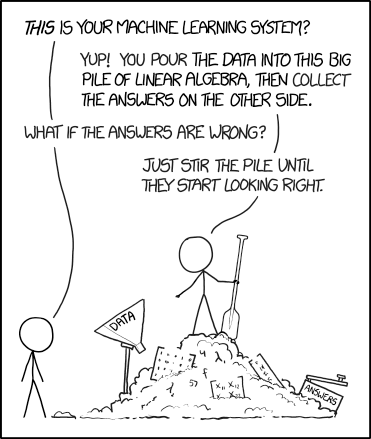
\includegraphics[width=4cm]{assets/machine_learning}
    \caption{The pile gets soaked with data and starts to get mushy over time, so it's technically recurrent.}
  \end{figure}
  \end{column}
\end{columns}
\end{frame}

%%%%%%%%%%%%%%%%%%%%%%%%%%%%%%%%%%%%%%%%%%%%%%%%%%%%%%%%%%%%%%%%%%%%%%%%%%%%%%%%

\section{Use Case: Extracting Tables from Images}

\begin{frame}
  \frametitle{Primer: What are we trying to accomplish}
  \begin{itemize}
    \item Tabular data is locked in PDFs
    \begin{itemize}
      \item Either as a typeset document
      \item Or as a scanned image
    \end{itemize}
    \item Sometimes copy \& paste won't suffice (or impossible with images)
    \item Let's take a quick look at the full pipeline to see where Seq2Seq models can fit in
  \end{itemize}
\end{frame}

\begin{frame}
  \frametitle{What is our data?}
  \begin{figure}
    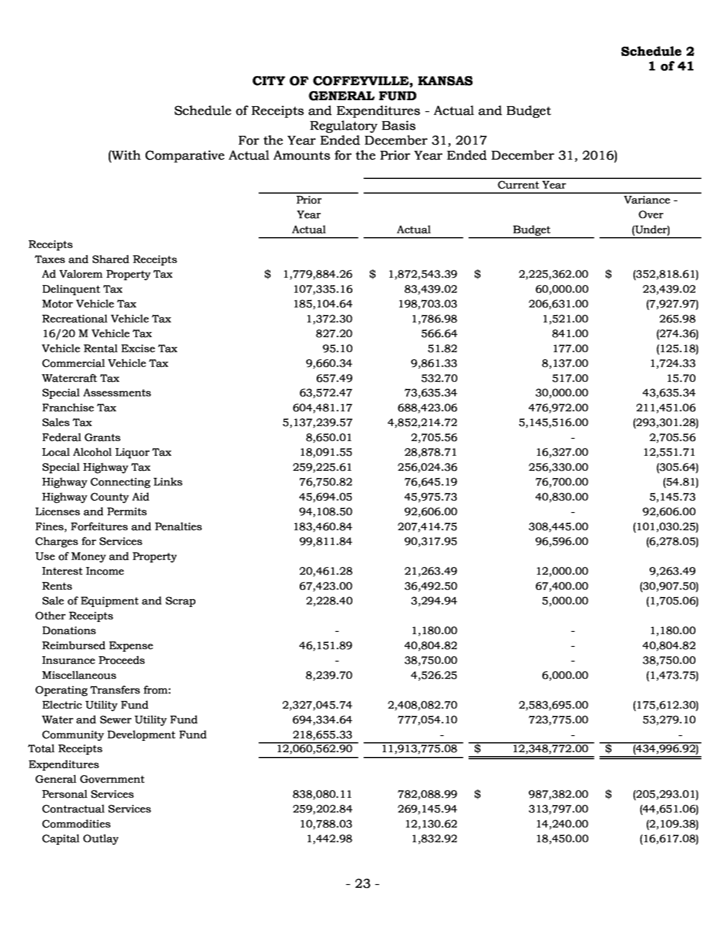
\includegraphics[width=3.5cm, valign=c]{assets/table_big}
    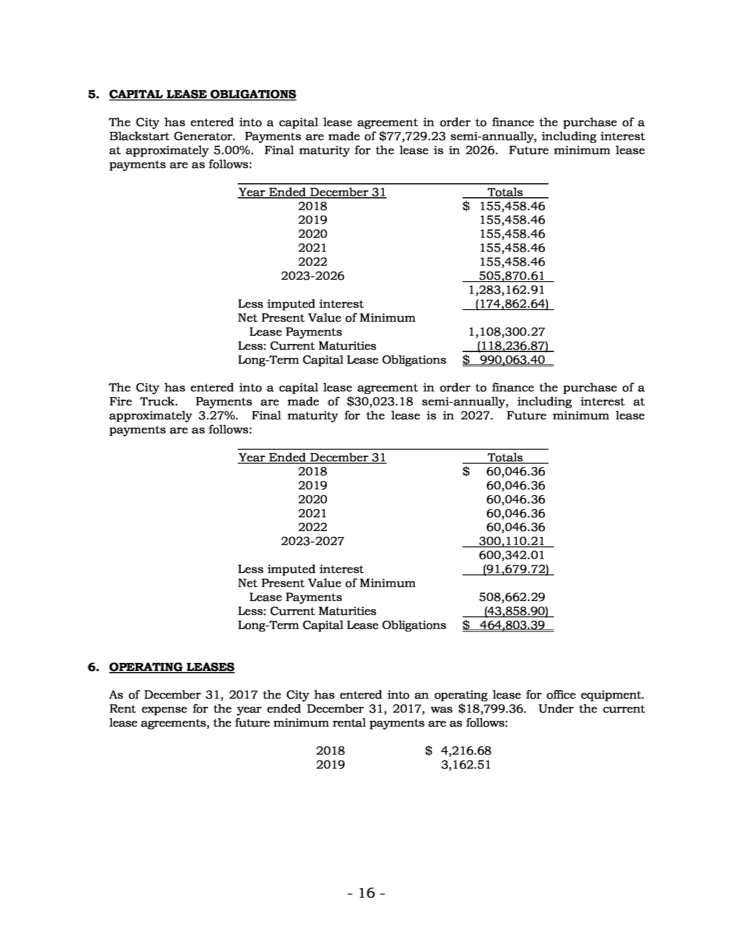
\includegraphics[width=3.5cm, valign=c]{assets/table_small}
    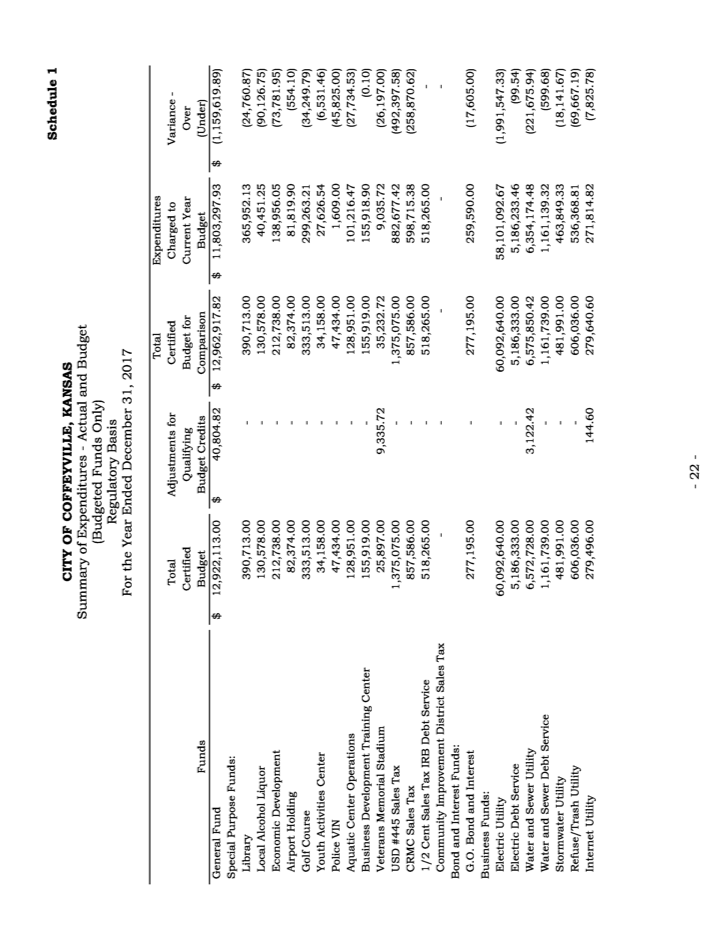
\includegraphics[width=3.5cm, valign=c]{assets/table_rotated}
  \end{figure}
\end{frame}

\begin{frame}
  \frametitle{Current Pipeline for Table Extraction}
  \begin{itemize}
    \item Convert to an Image
    \item Binary Page Classification: Is there a table on this page?
    \item Table Segmentation: U-Net Model
    \item Optical Character Recognition via Tesseract
    \item \textbf{Column Segmentation}
    \item Table Alignment
    \item Dump to CSV
  \end{itemize}
\end{frame}

\begin{frame}
  \frametitle{Visual: Table Segmentation}
  \begin{figure}
    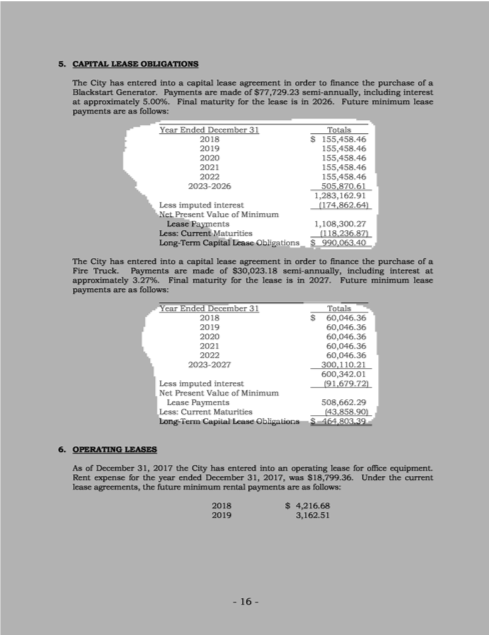
\includegraphics[width=3.5cm, valign=c]{assets/mask1}
    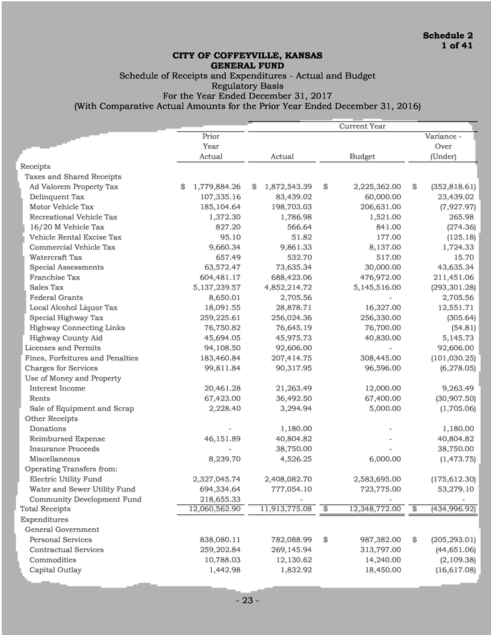
\includegraphics[width=3.5cm, valign=c]{assets/mask2}
    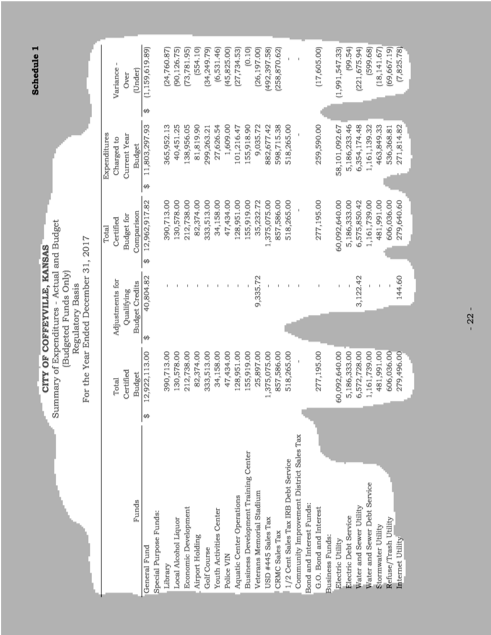
\includegraphics[width=3.5cm, valign=c]{assets/mask3}
  \end{figure}
\end{frame}

\begin{frame}
  \frametitle{Visual: Tesseract OCR Output}
  \begin{figure}
    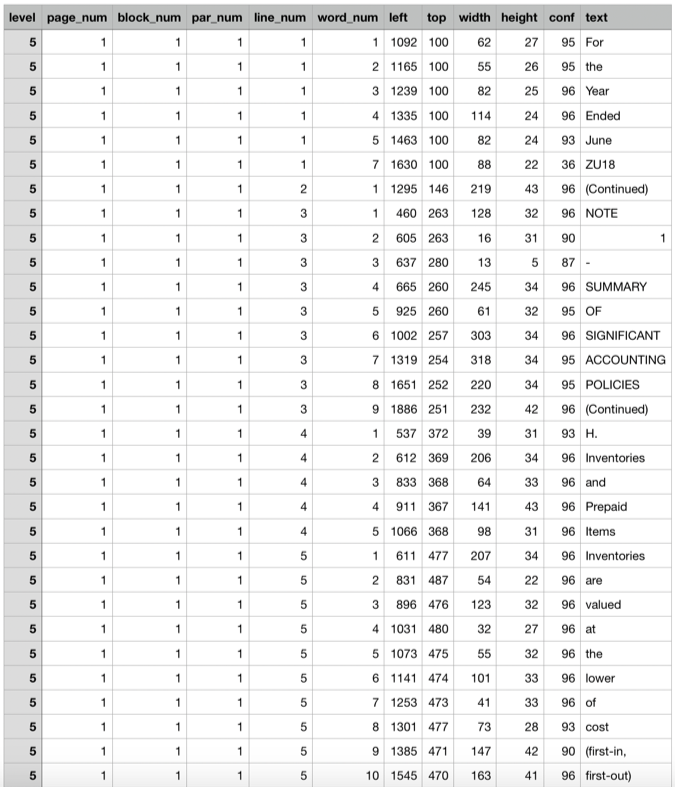
\includegraphics[height=7.5cm, valign=c]{assets/tesseract}
  \end{figure}
\end{frame}

\begin{frame}
  \frametitle{Column Segmentation}
  \begin{itemize}
    \item Naive approach is to merge words close together
    \begin{itemize}
      \item But spacing is \textbf{variable} in tables
      \item Text justification (left, center, right)
    \end{itemize}
    \item \textbf{Union Find} to group columns by \textbf{Intersection Over Union (IOU)}
    \begin{figure}
      
\includegraphics[width=4.25cm, valign=c]{assets/uf1}
      $\longrightarrow$
      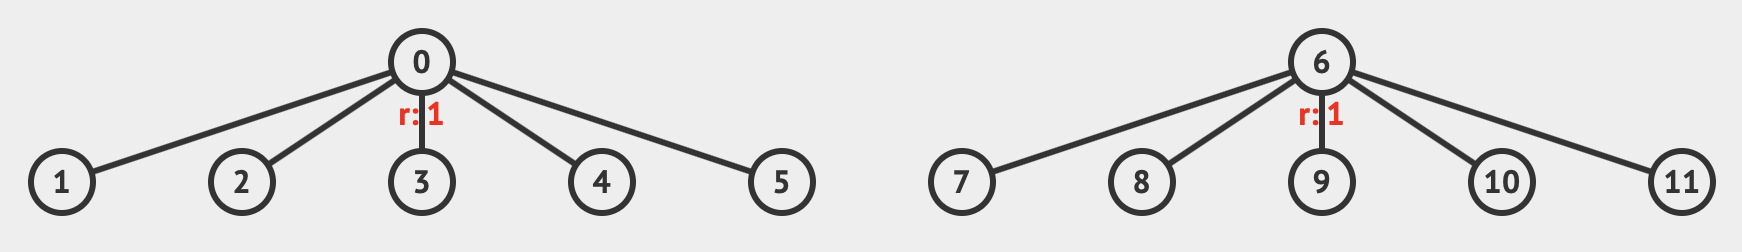
\includegraphics[width=4.25cm, valign=c]{assets/uf2}
    \end{figure}
    \pause
    \item \textbf{Idea:} Use a Seq2Seq to learn correct segmentation
  \end{itemize}
\end{frame}

\begin{frame}
  \frametitle{Visual: Alignment}
  \begin{figure}
    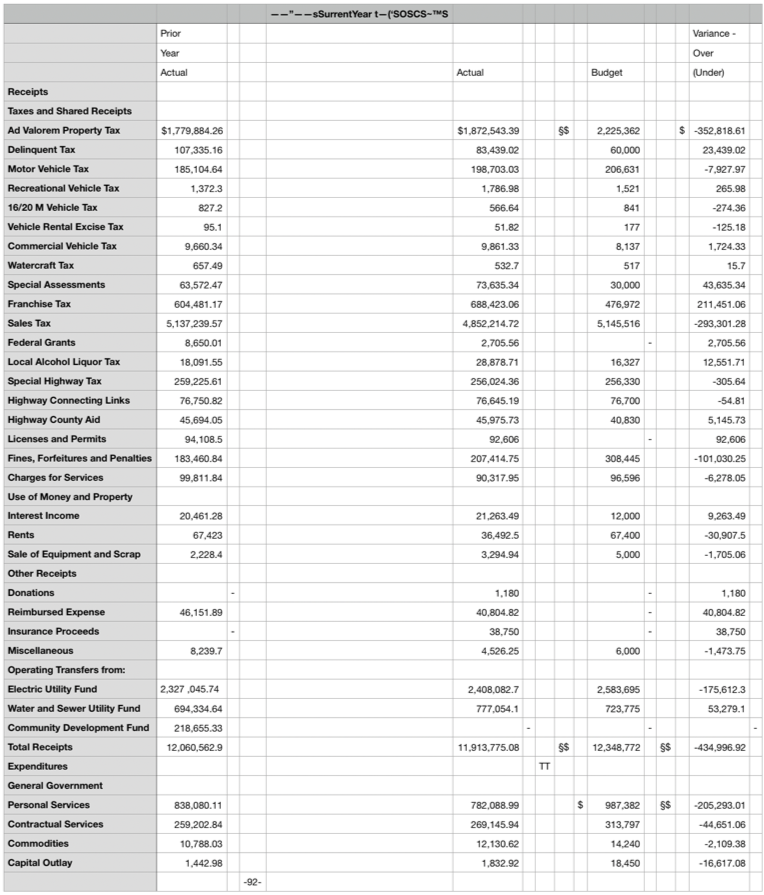
\includegraphics[height=7.5cm, valign=c]{assets/result1}
  \end{figure}
\end{frame}

\begin{frame}
  \frametitle{Problem Statement: Column Segmentation}
  \begin{figure}
    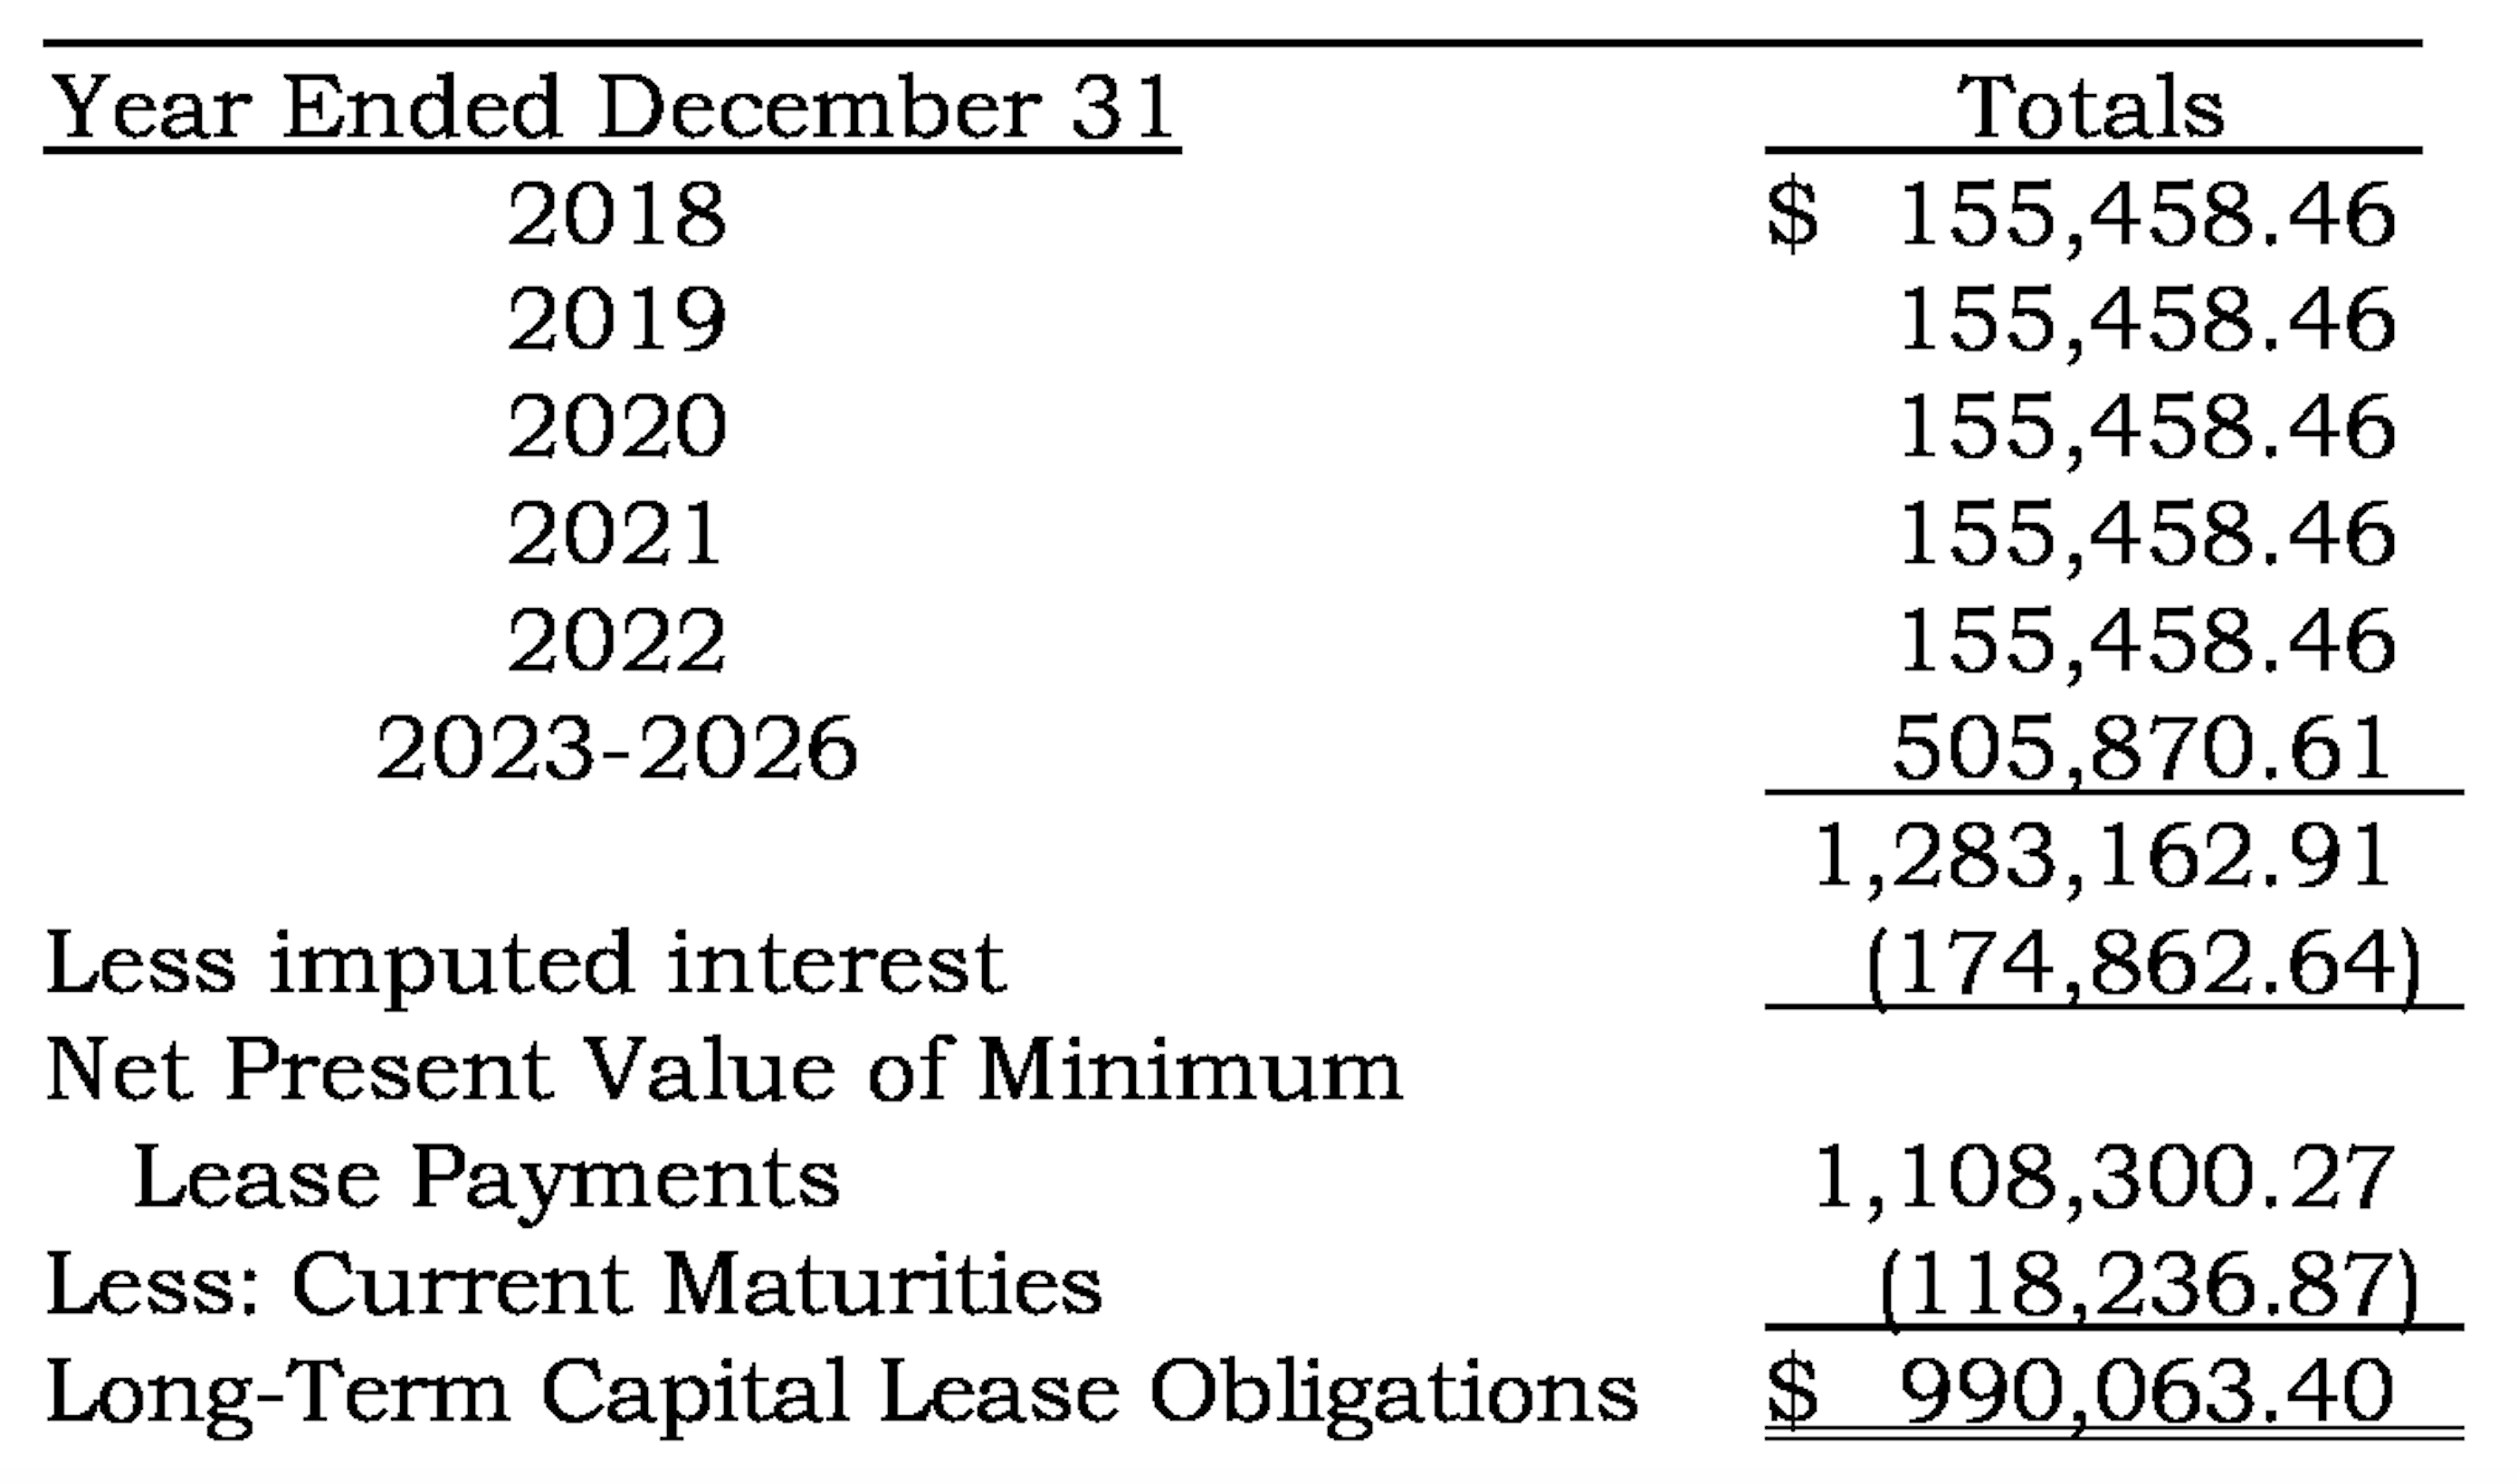
\includegraphics[width=4.25cm, valign=c]{assets/table}
    $\longrightarrow$
    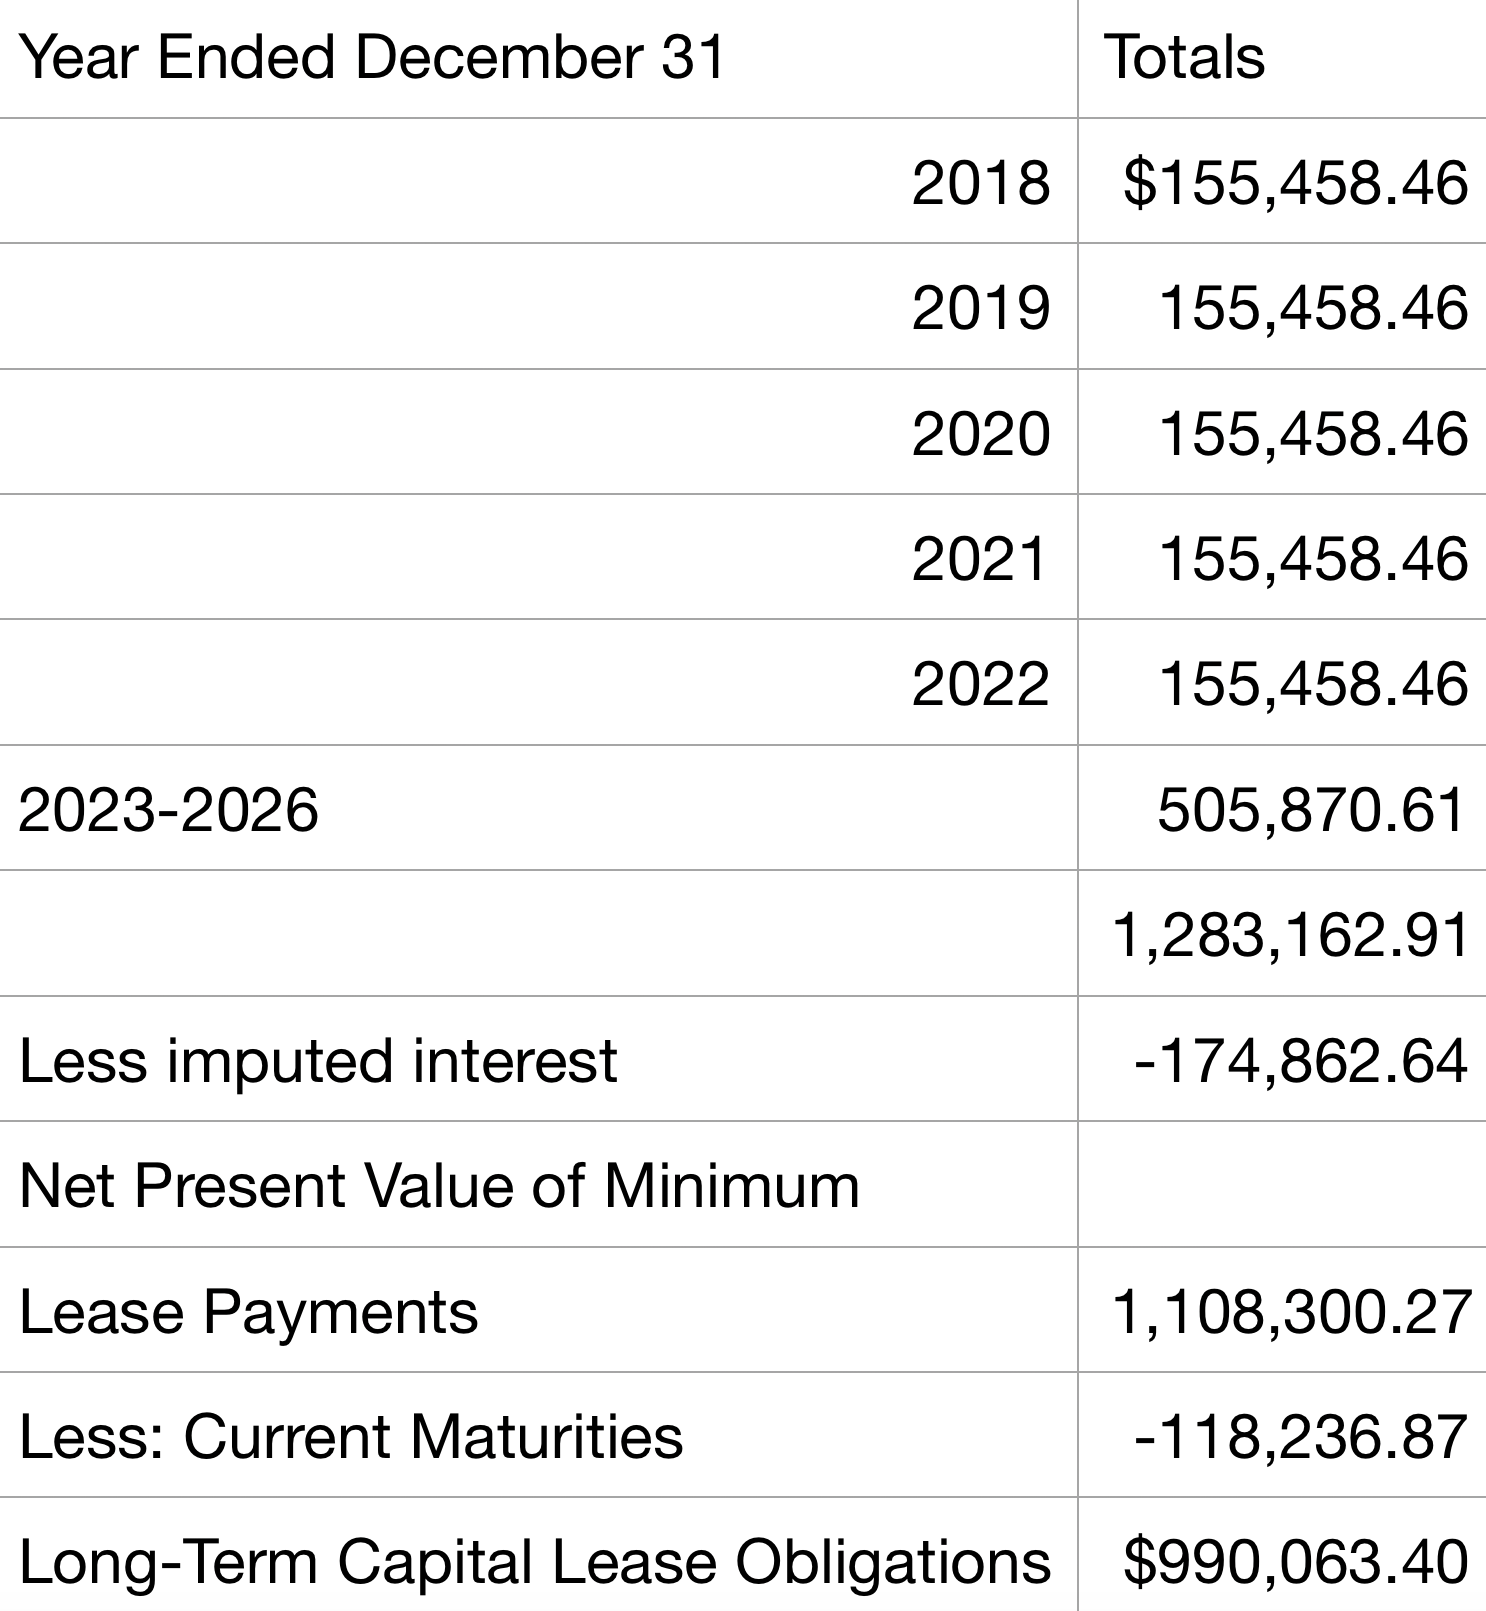
\includegraphics[width=4.25cm, valign=c]{assets/csv}
  \end{figure}
  \begin{itemize}
    \item Given a sequence of text, can we predict where to insert columns?
  \end{itemize}
\end{frame}

\begin{frame}
  \frametitle{Revisiting Column Segmentation as a Seq2Seq Problem}
  \begin{itemize}
    \item Translation Task
    \item Given a sequence of tokens
    \item Translate into the same set of tokens, but with a special \textcolor{WildStrawberry}{$\langle \texttt{SEG} \rangle$} token
  \end{itemize}
  \vspace{5mm}
  \begin{equation*}
    \centering
    \textcolor{ForestGreen}{
    \begin{array}{ccccccc}
      \texttt{Less} & \texttt{imputed} & \texttt{interest} & {} & \texttt{(} & \texttt{174,862.64} & \texttt{)} \\
      {} & {} & {} & \textcolor{BrickRed}{\big\Downarrow} & {} & {} & {} \\
      \texttt{Less} & \texttt{imputed} & \texttt{interest} & \textcolor{WildStrawberry}{\langle\texttt{SEG}\rangle} & \texttt{(} & \texttt{174,862.64} & \texttt{)} \\
    \end{array}}
  \end{equation*}
\end{frame}

\begin{frame}
  \frametitle{Seq2Seq Architecture}
  \begin{figure}
    \centering
    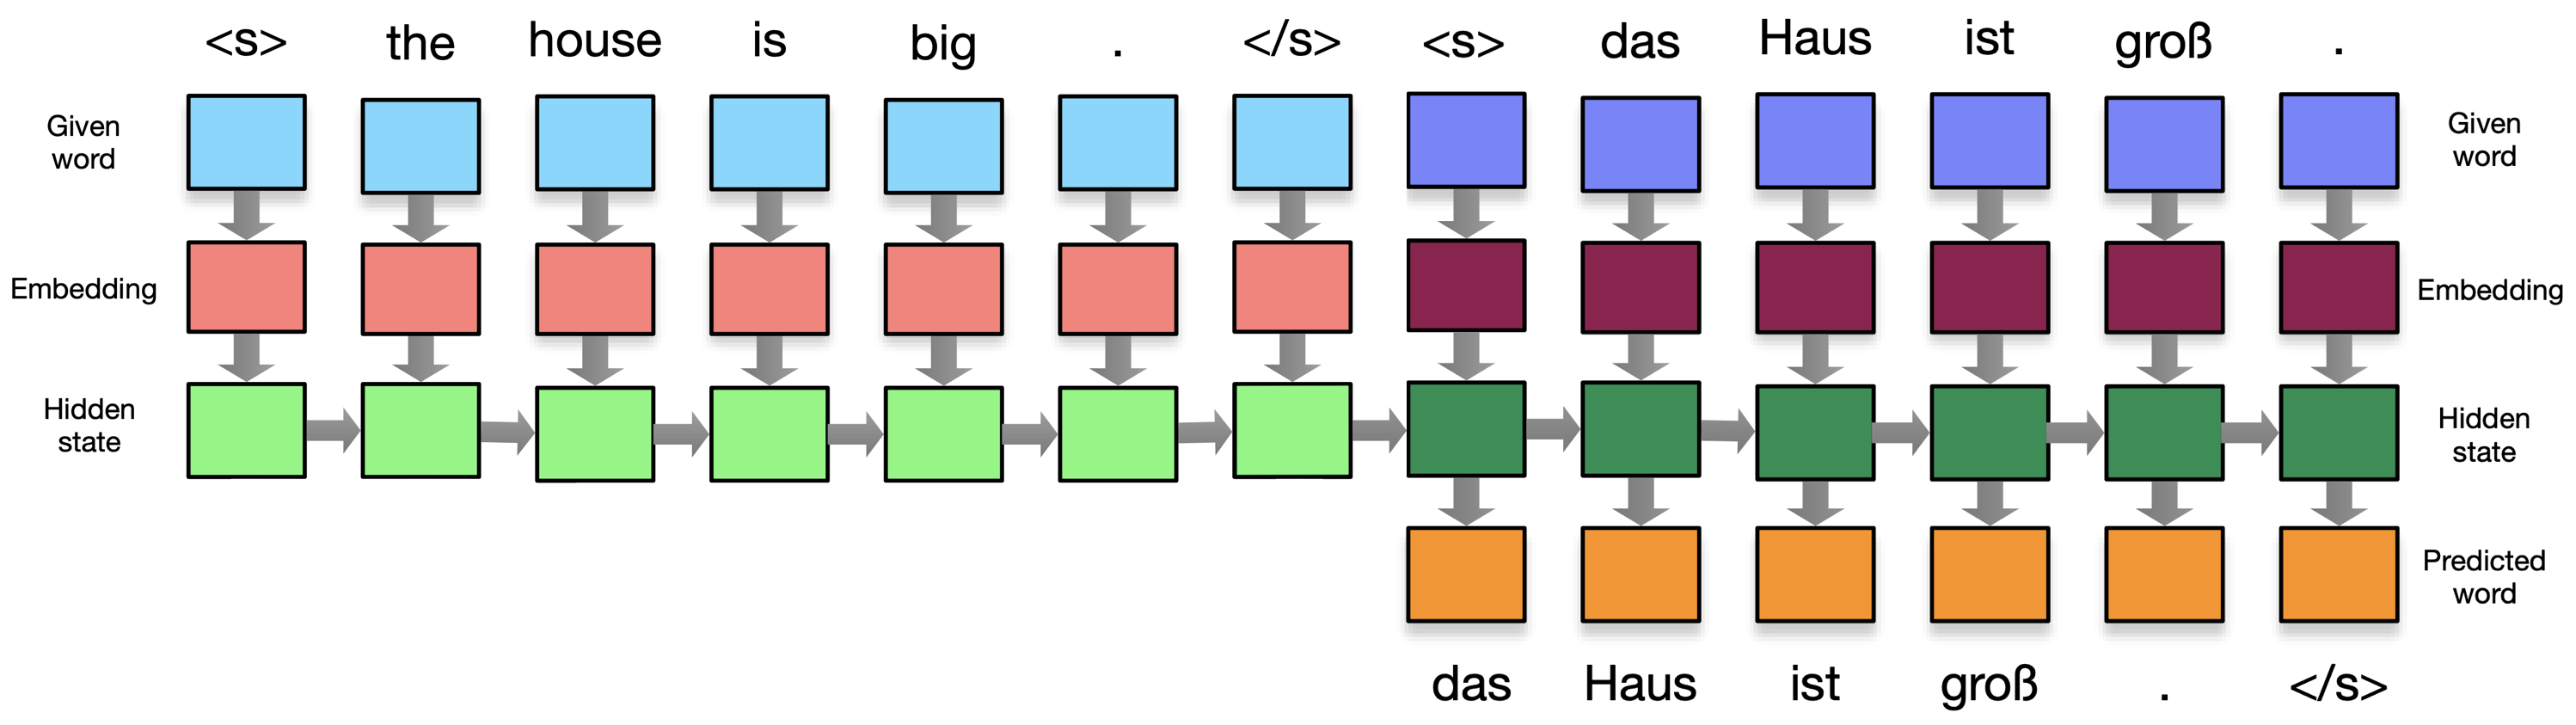
\includegraphics[width=10cm, valign=c]{assets/enc-dec}
  \end{figure}
  % add picture from notebook
  \begin{itemize}
    \item We can use a \textbf{Encoder-Decoder} style model!
  \end{itemize}
\end{frame}

%%%%%%%%%%%%%%%%%%%%%%%%%%%%%%%%%%%%%%%%%%%%%%%%%%%%%%%%%%%%%%%%%%%%%%%%%%%%%%%%
\section{Encoder-Decoder Architecture}

\begin{frame}
\frametitle{Overview: Encoders and Decoders}
\begin{itemize}
  \item We have 2 sub-networks: an \textbf{Encoder} and a \textbf{Decoder}
  \item Encoders
  \begin{itemize}
    \item Give the source sentence meaning
  \end{itemize}
  \item Decoders
  \begin{itemize}
    \item Emit a variable-length sequence
  \end{itemize}
  \item We will discuss how to connect the two for joint training
\end{itemize}
\end{frame}

\begin{frame}
\frametitle{Overview: Encoders and Decoders}
\begin{figure}
  \centering
  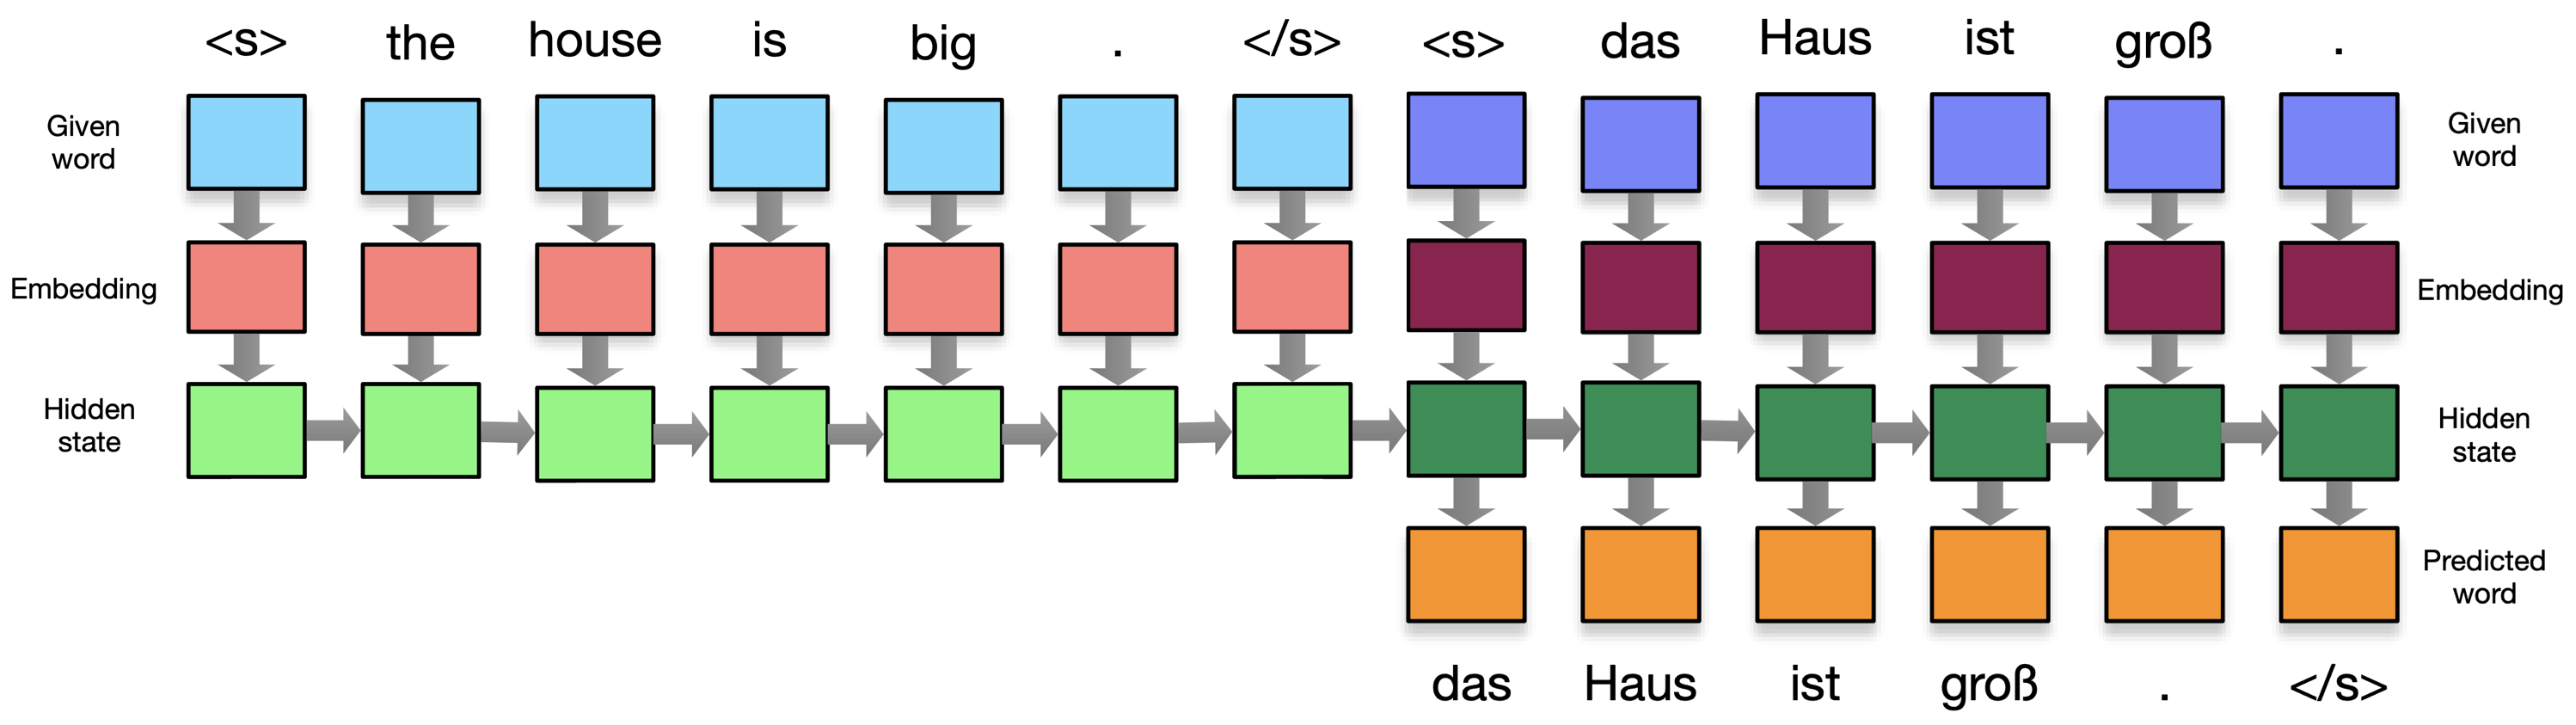
\includegraphics[width=10cm, valign=c]{assets/enc-dec}
\end{figure}
\begin{itemize}
  \item Encapsulation allows for flexible design choices
  \item \textbf{Embeddings}
    \begin{itemize}
      \item Pre-trained
      \item DIY
    \end{itemize}
  \item \textbf{Recurrent Layer}
    \begin{itemize}
      \item Type
      \item Depth
      \item Directionality
    \end{itemize}
\end{itemize}
\end{frame}

\begin{frame}
\frametitle{What makes an Encoder?}
\begin{figure}
  \centering
  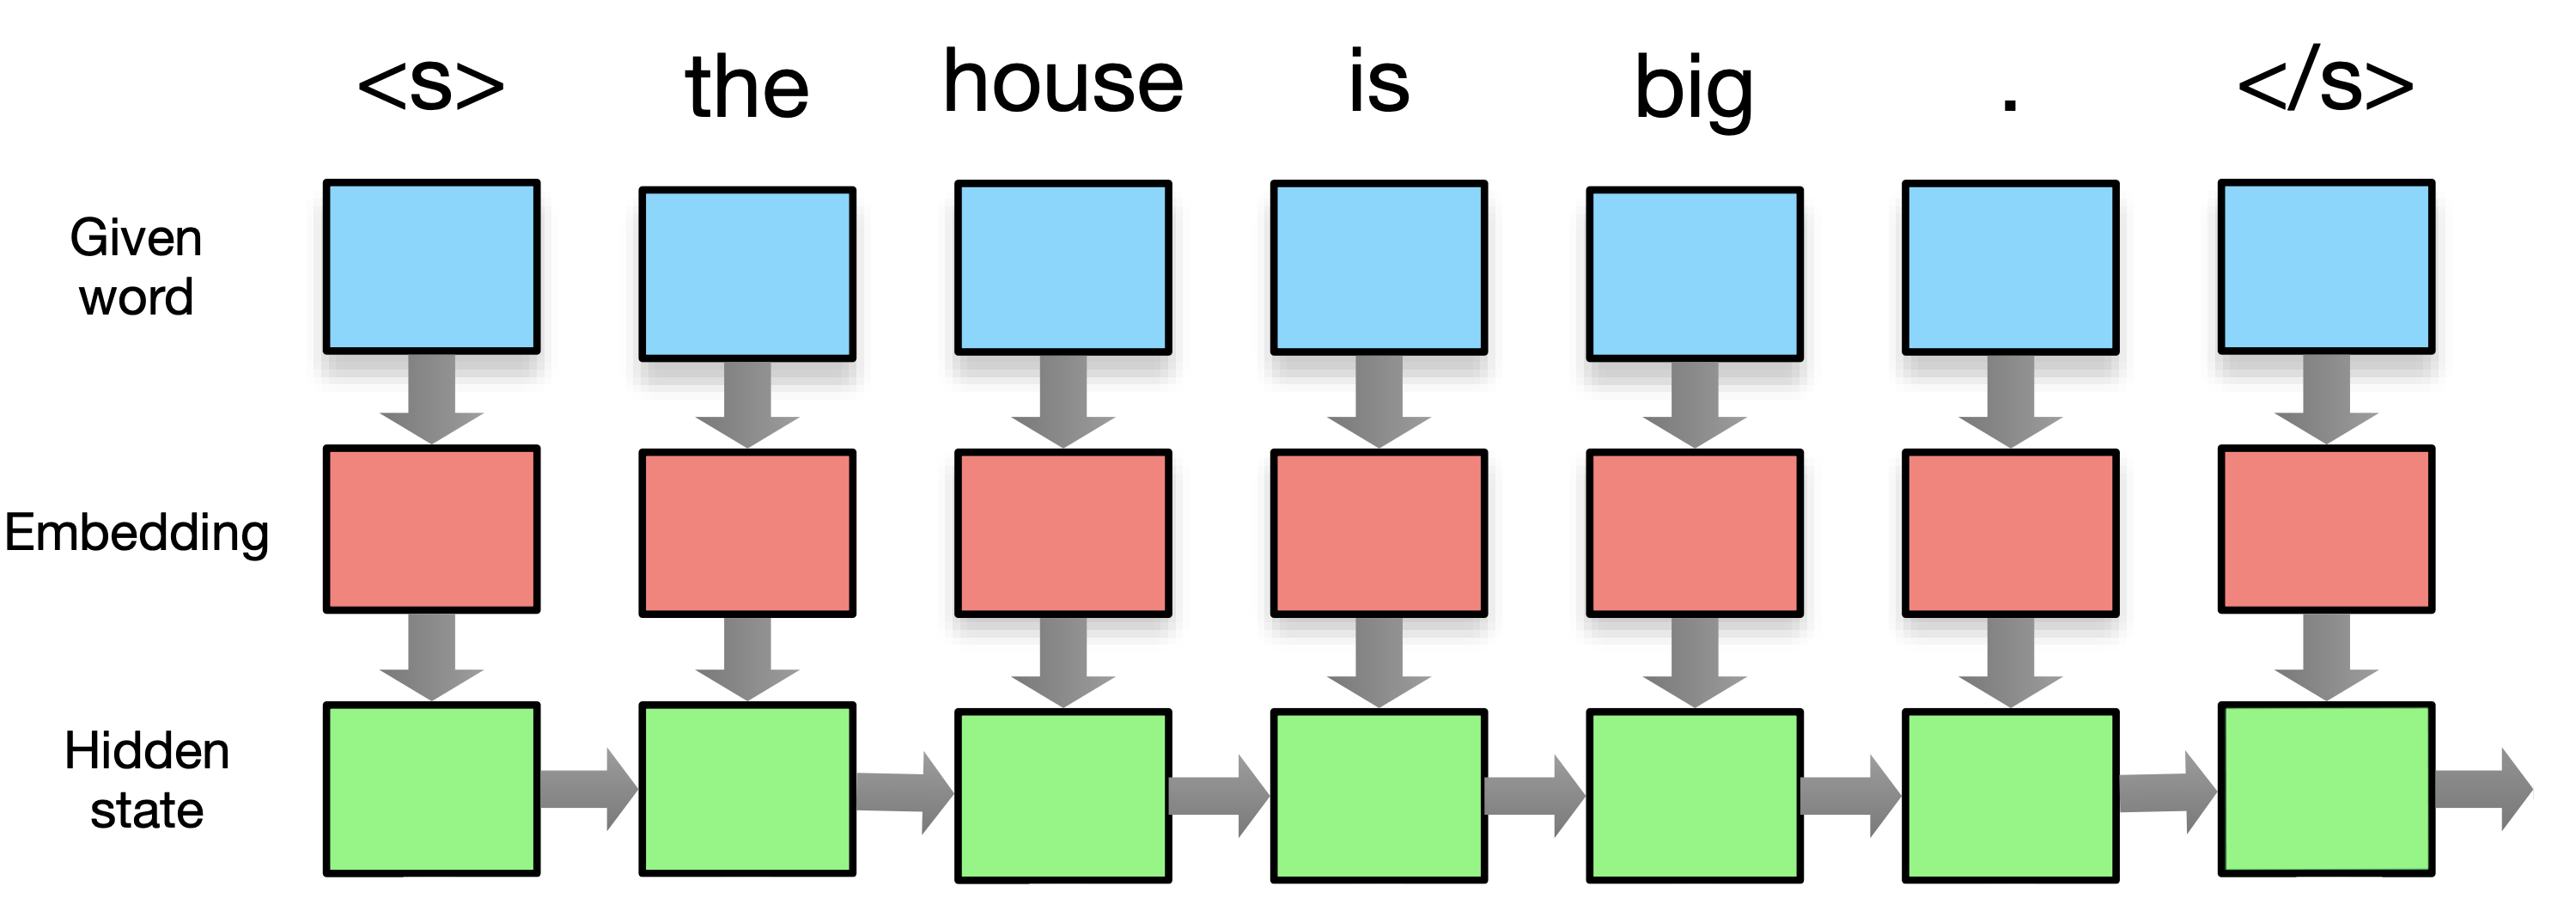
\includegraphics[width=10cm, valign=c]{assets/encoder}
\end{figure}
\begin{itemize}
  \item Recall: \textbf{Encoders} give the source sentence meaning
  \item Effectively a language model, without a layer to predict the next word
  \item Idea is to pass on the hidden state, and possibly use the encodings directly
\end{itemize}
\end{frame}

\begin{frame}
\frametitle{What makes a Decoder?}
\begin{figure}
  \centering
  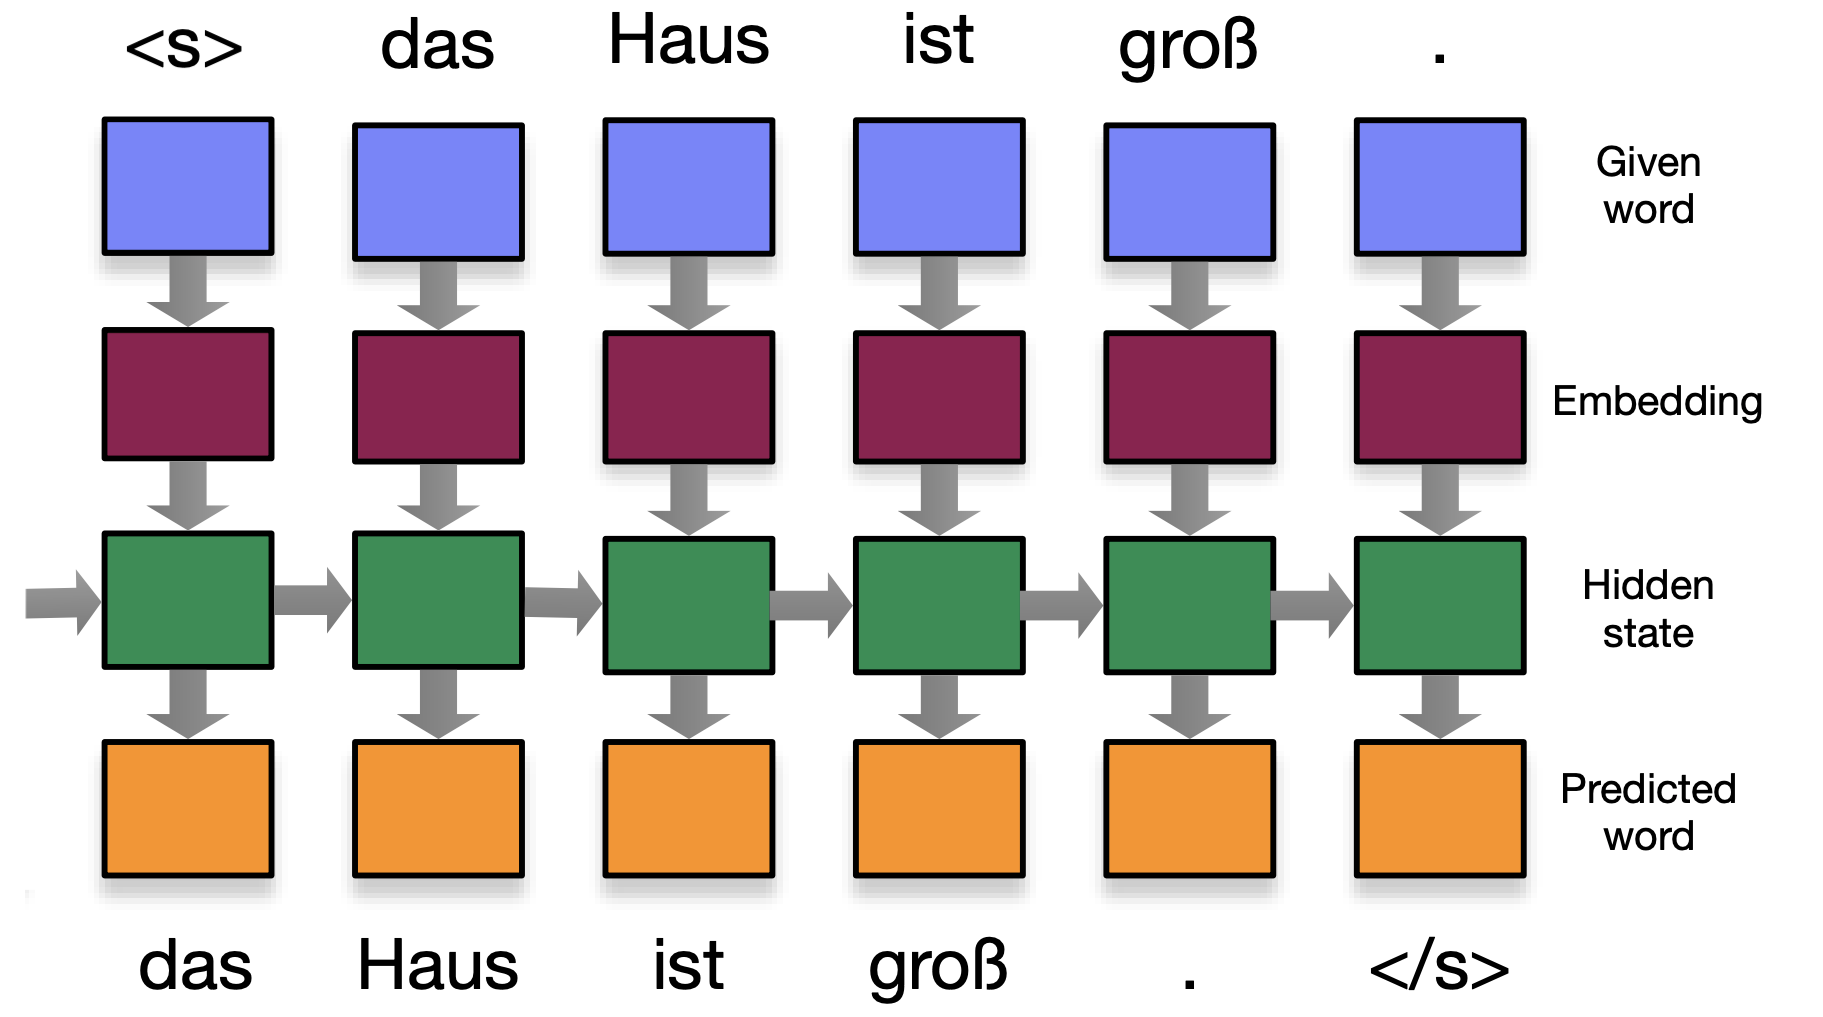
\includegraphics[width=8cm, valign=c]{assets/decoder}
\end{figure}
\begin{itemize}
  \item Recall: \textbf{Decoders} provide a new sequence conditioned on the Encoder's hidden state
  \item Starts with the Encoder's hidden state, and predicts one token at a time
  \item Re-feed the predicted token back into the decoder
\end{itemize}
\end{frame}


%%%%%%%%%%%%%%%%%%%%%%%%%%%%%%%%%%%%%%%%%%%%%%%%%%%%%%%%%%%%%%%%%%%%%%%%%%%%%%%%
\section{Word Embeddings: Practical Considerations}

\begin{frame}
  \frametitle{Column Segmentation Issue: Vocabulary Size}
  \begin{itemize}
    \item Is the text actually important?
    \item Over \textbf{10K unique tokens}, mostly numbers
    \pause
    \item \textbf{Solutions:}
    \begin{itemize}
      \item Token $\rightarrow$ Part-of-Speech
      \item Numeric Value $\rightarrow$ \textcolor{Fuchsia}{$\langle \texttt{NUM} \rangle$}
    \end{itemize}
    \item Reduces vocabulary size to \textbf{21 tokens}
    \item But lets take a look at alternative solutions to managing vocab size
  \end{itemize}
  % picture of table
\end{frame}

\begin{frame}
  \frametitle{Recap: Word Embeddings}
  \begin{equation*}
    \begin{array}{rc}
      \textcolor{Fuchsia}{\texttt{the}} & \rightarrow \\
      \textcolor{WildStrawberry}{\texttt{cat}} & \rightarrow \\
      \textcolor{BurntOrange}{\texttt{is}} & \rightarrow \\
      \textcolor{Emerald}{\texttt{black}} & \rightarrow \\
    \end{array}
    \begin{bmatrix*}[r]
          \textcolor{Fuchsia}{\texttt{1.23}} & \textcolor{Fuchsia}{\texttt{-0.58}} & \textcolor{Fuchsia}{\texttt{0.22}} & \textcolor{Fuchsia}{\texttt{-0.80}} & \textcolor{Fuchsia}{\texttt{0.61}} \\
          \textcolor{WildStrawberry}{\texttt{-1.10}} & \textcolor{WildStrawberry}{\texttt{1.23}} & \textcolor{WildStrawberry}{\texttt{0.17}} & \textcolor{WildStrawberry}{\texttt{-0.21}} & \textcolor{WildStrawberry}{\texttt{1.43}} \\
          \textcolor{BurntOrange}{\texttt{-0.26}} & \textcolor{BurntOrange}{\texttt{0.70}} & \textcolor{BurntOrange}{\texttt{0.27}} & \textcolor{BurntOrange}{\texttt{0.59}} & \textcolor{BurntOrange}{\texttt{-1.04}} \\
          \textcolor{Emerald}{\texttt{-1.13}} & \textcolor{Emerald}{\texttt{-0.81}} & \textcolor{Emerald}{\texttt{-0.53}} & \textcolor{Emerald}{\texttt{-0.59}} & \textcolor{Emerald}{\texttt{0.26}} \\
    \end{bmatrix*}
  \end{equation*}
  \begin{itemize}
    \item A trick to map tokens to vector representations
  \end{itemize}
\end{frame}


\begin{frame}
\frametitle{Recap: Pretrained Word Embeddings}
\begin{itemize}
  \item Co-occurence Matrix
  \item Pointwise Mutual Information
  \item SVD Co-occurence
  \item Ngram
  \item CBOW, Skip Gram
  \item GloVe
  \item ELMo
  \item BERT
\end{itemize}

\end{frame}


\begin{frame}
\frametitle{DIY Embeddings}
\begin{itemize}
  \item We can always train our own!
\end{itemize}
\end{frame}

\begin{frame}
\frametitle{Special Tokens for Sequence Modeling}
\begin{itemize}
  \item $\textcolor{WildStrawberry}{\langle \texttt{PAD} \rangle}$ $\rightarrow$ Padding / Masking
  \item $\textcolor{Periwinkle}{\langle \texttt{UNK} \rangle}$ $\rightarrow$ Unknown words
  \item $\textcolor{ForestGreen}{\langle \texttt{SOS} \rangle}$ $\rightarrow$ Start of Sentence
  \item $\textcolor{BrickRed}{\langle \texttt{EOS} \rangle}$ $\rightarrow$ End of Sentence
\end{itemize}
\vspace{5mm}
\begin{equation*}
  \centering
  \begin{array}{cccccccc}
    \textcolor{ForestGreen}{\langle \texttt{SOS} \rangle} & \texttt{Data} & \texttt{Science} & \texttt{is} & \texttt{the} & \textcolor{Periwinkle}{\langle \texttt{UNK} \rangle} & \texttt{!} & \textcolor{BrickRed}{\langle \texttt{EOS} \rangle} \\
    \textcolor{ForestGreen}{\langle \texttt{SOS} \rangle} & \texttt{I}      & \textcolor{Periwinkle}{\langle \texttt{UNK} \rangle} & \texttt{for} & \texttt{S\&P} & . & \textcolor{BrickRed}{\langle \texttt{EOS} \rangle} & \textcolor{WildStrawberry}{\langle \texttt{PAD} \rangle}  \\
    \textcolor{ForestGreen}{\langle \texttt{SOS} \rangle} & \texttt{Hello}  & \texttt{World} & ! & \textcolor{BrickRed}{\langle \texttt{EOS} \rangle} & \textcolor{WildStrawberry}{\langle \texttt{PAD} \rangle} & \textcolor{WildStrawberry}{\langle \texttt{PAD} \rangle} & \textcolor{WildStrawberry}{\langle \texttt{PAD} \rangle}
  \end{array}
\end{equation*}
\end{frame}

\begin{frame}
\frametitle{Mangaging the Vocab Size}
\begin{columns}
  \begin{column}{0.45\textwidth}
    \begin{itemize}
      \item Languages are unevenly distributed
      \item Many rare words, names $\rightarrow$ inflates the size of the vocabulary
      \item \textbf{Problem:}
      \begin{itemize}
        \item Large embedding matrices for source, target language
        \item Large output layers for prediction and softmax
      \end{itemize}
      \item Naive Solution: Limit the vocab size to most frequent
    \end{itemize}
  \end{column}
  \begin{column}{0.45\textwidth}
    \begin{figure}
      \centering
      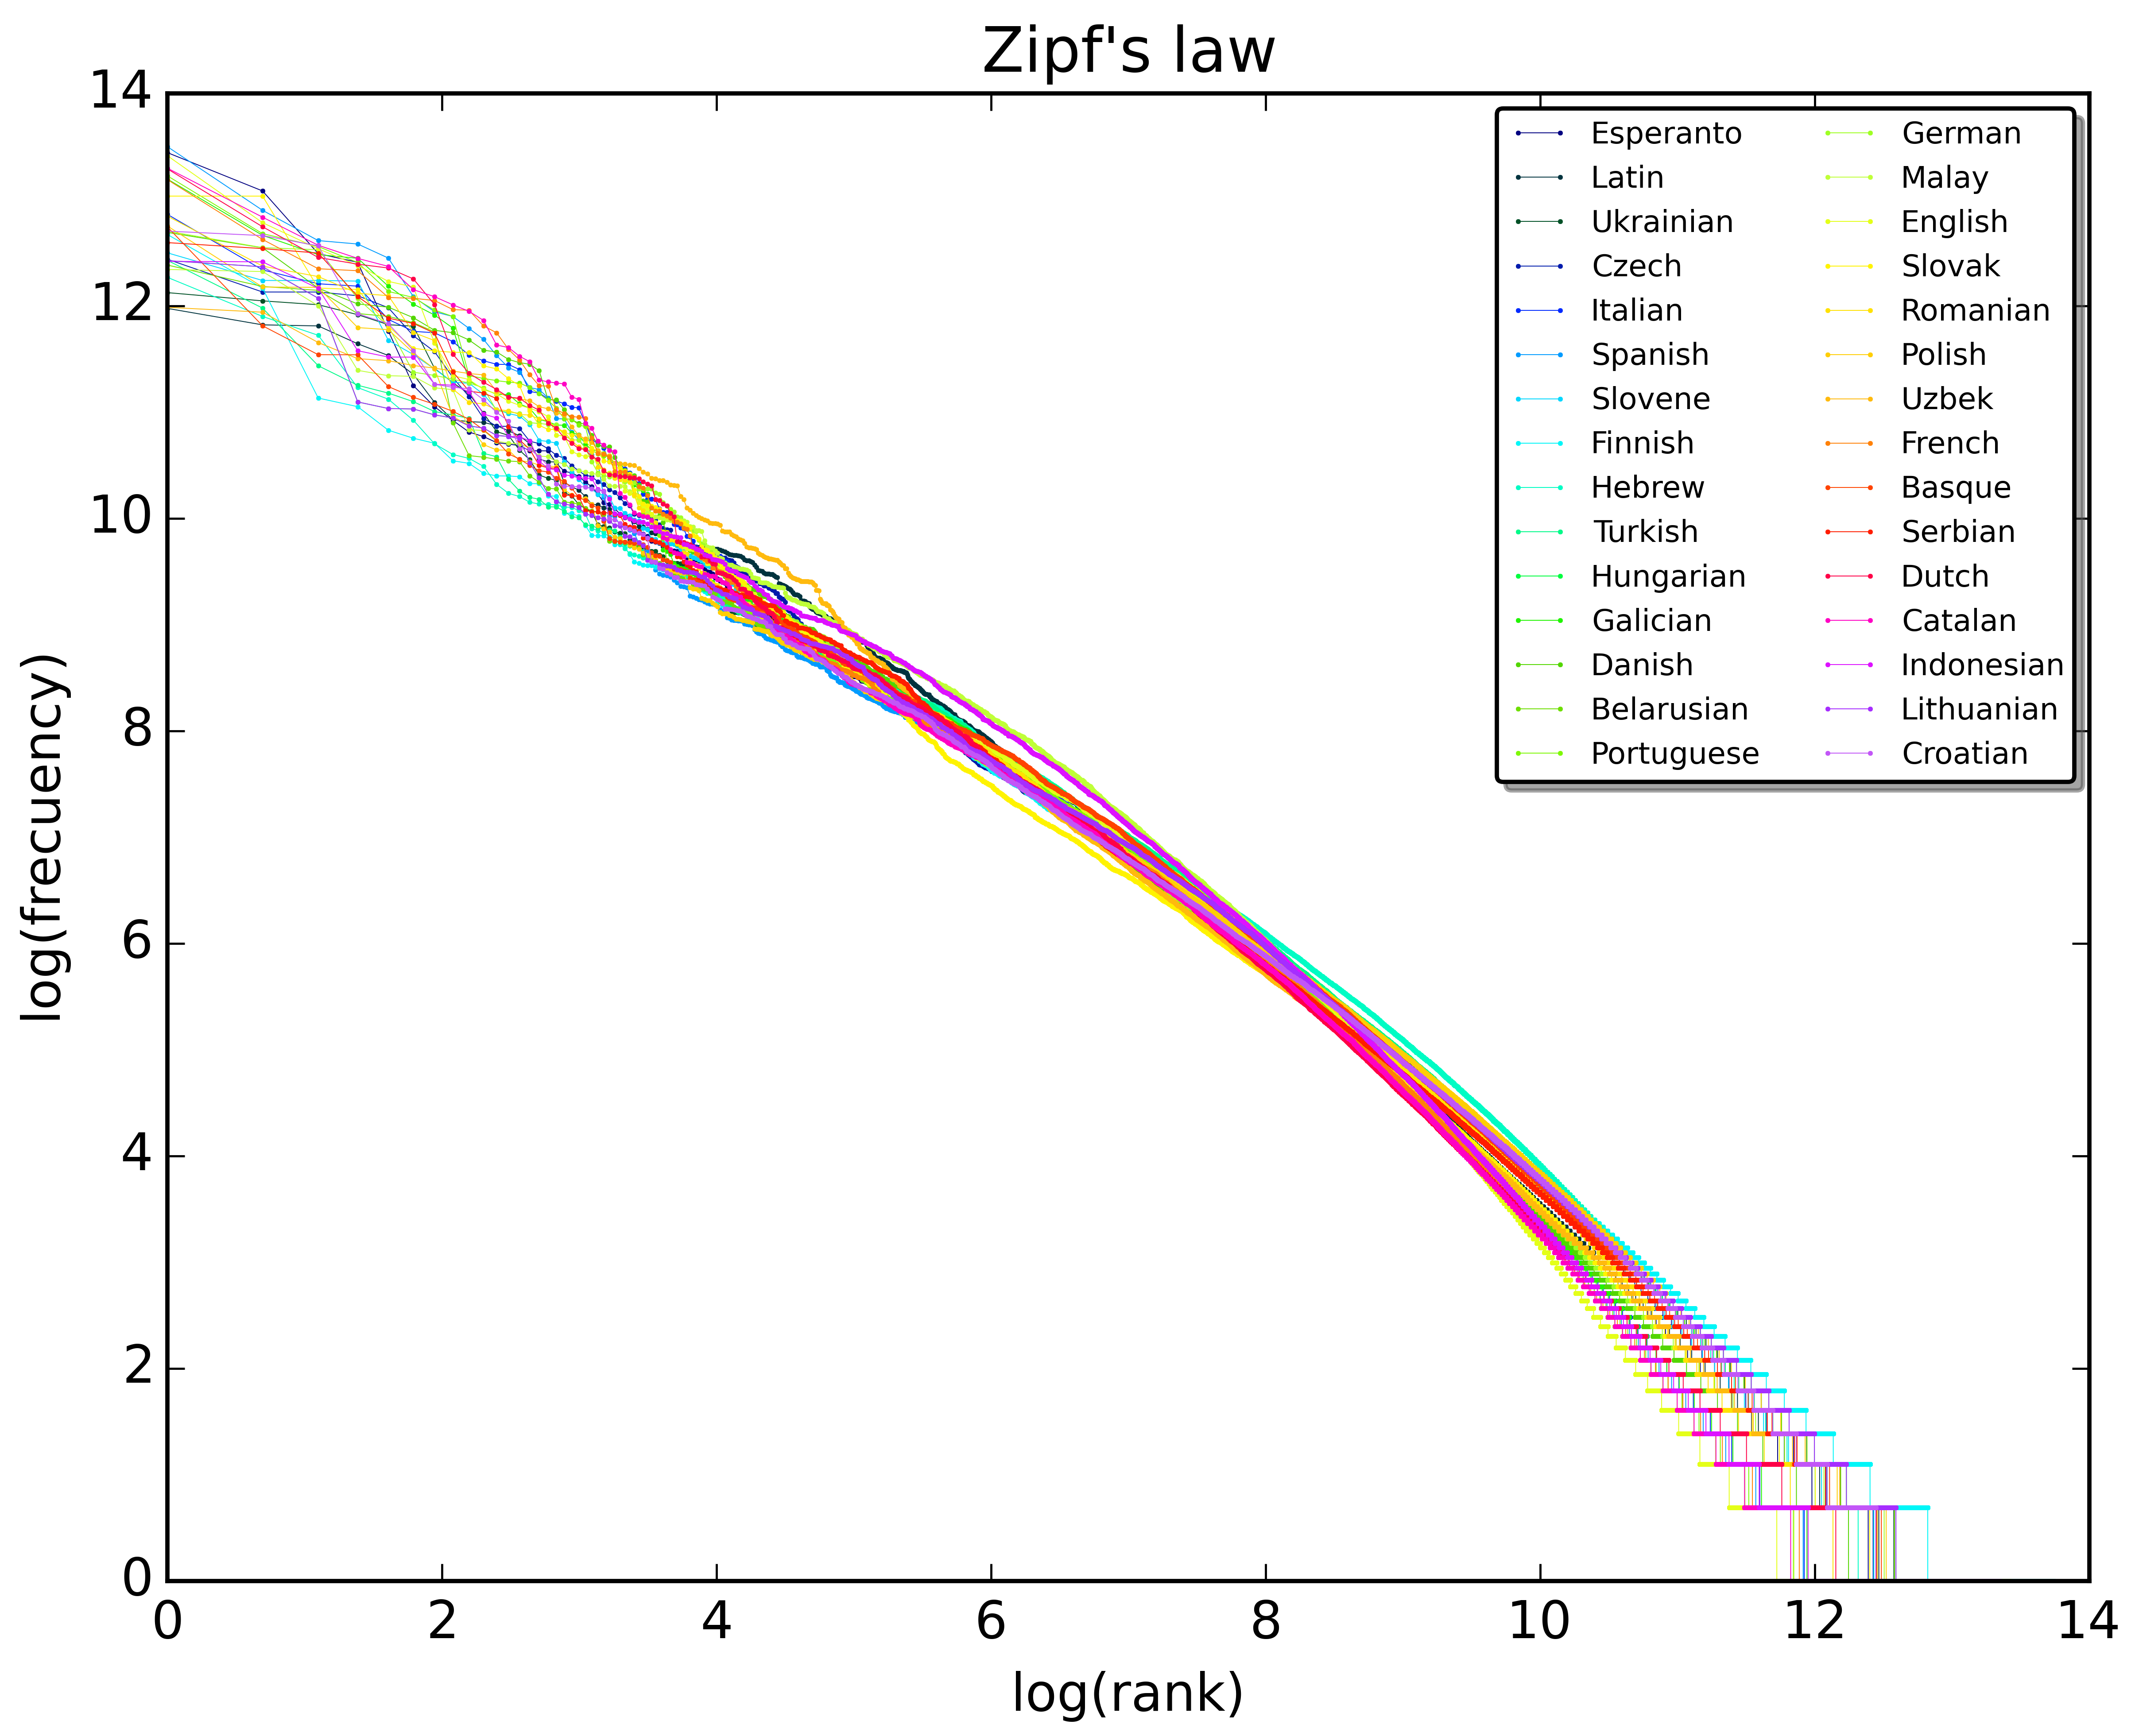
\includegraphics[width=4.5cm, valign=c]{assets/zipf}
      \vspace{5mm}
      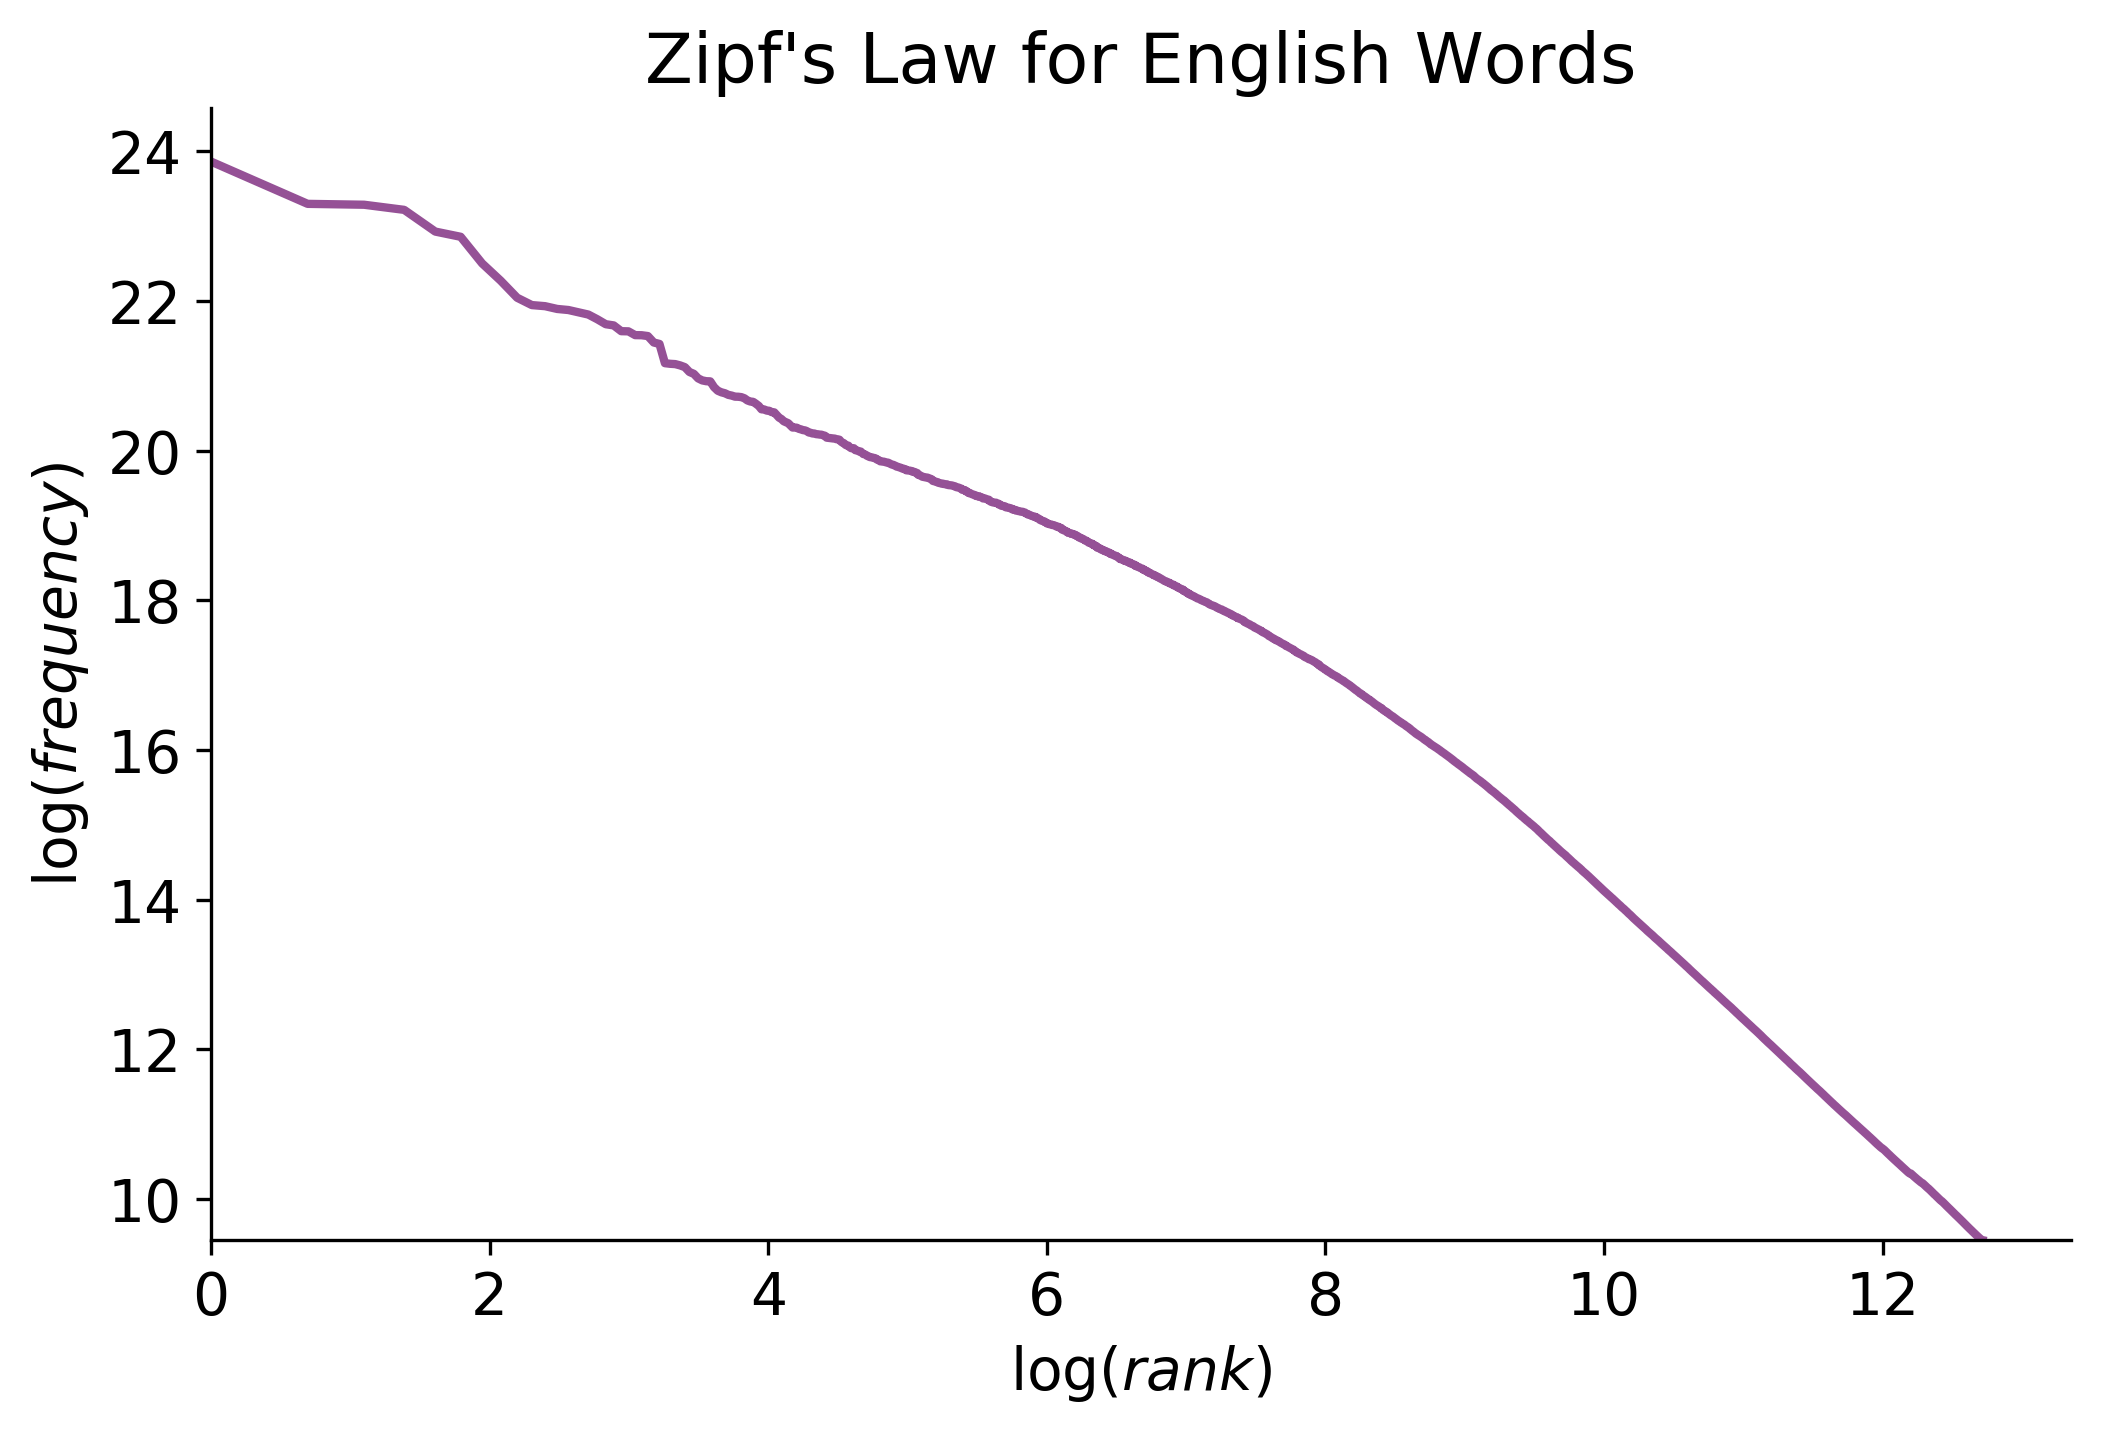
\includegraphics[width=4.5cm, valign=c]{assets/zipf_log}
    \end{figure}
  \end{column}
\end{columns}
% graph of zipfs law
\end{frame}

\begin{frame}
\frametitle{Morphology, Compounding, and Transliteration}
\begin{itemize}
  \item Morphological Analysis
  \begin{equation*}
    \textcolor{Fuchsia}{tweet, tweets, tweeted, tweeting, retweet, \hdots}
  \end{equation*}
  \item Compound Splitting
  \begin{itemize}
    \item \textcolor{Fuchsia}{homework} $\rightarrow$ \textcolor{Fuchsia}{home$\cdotp$work}
    \item \textcolor{Fuchsia}{website} $\rightarrow$ \textcolor{Fuchsia}{web$\cdotp$site}
  \end{itemize}
  \item Names, Places, Proper Nouns
  \begin{itemize}
    \item \textcolor{Fuchsia}{Hoboken, Baltimore, Obama, Michelle}
    \item Can do Transliteration
  \end{itemize}
\end{itemize}
\end{frame}

\begin{frame}
\frametitle{Handling Numbers}
\begin{itemize}
  \item Do we really need to encode every number? \textbf{NO!}
\end{itemize}
  \begin{equation*}
    \texttt{I pay $\textcolor{Fuchsia}{950.00}$ in May $\textcolor{Fuchsia}{2007}$} \;>\; \texttt{I pay $\textcolor{Fuchsia}{2007}$ in May $\textcolor{Fuchsia}{950.00}$}
  \end{equation*}
  \pause
\begin{itemize}
  \item \textbf{Solution 1:} Replace with a $\textcolor{Fuchsia}{\langle \texttt{NUM} \rangle }$ token, but
\end{itemize}
  \begin{equation*}
    \texttt{I pay $\textcolor{Fuchsia}{\langle \texttt{NUM} \rangle }$ in May $\textcolor{Fuchsia}{\langle \texttt{NUM} \rangle }$} \;=\; \texttt{I pay $\textcolor{Fuchsia}{\langle \texttt{NUM} \rangle }$ in May $\textcolor{Fuchsia}{\langle \texttt{NUM} \rangle }$}
  \end{equation*}
  \pause
\begin{itemize}
  \item \textbf{Solution 2:} Replace each digit with a unique symbol, e.g. \textcolor{Fuchsia}{$\texttt{5}$}
\end{itemize}
  \begin{equation*}
    \texttt{I pay \textcolor{Fuchsia}{555.55} in May \textcolor{Fuchsia}{5555} } \;>\; \texttt{I pay \textcolor{Fuchsia}{5555} in May \textcolor{Fuchsia}{555.55} }
  \end{equation*}
\begin{itemize}
  \item This reduces the need for embeddings, when we can simply do transliteration
\end{itemize}
\end{frame}

\begin{frame}
\frametitle{Factored Decomposition}
\begin{figure}
  \centering
  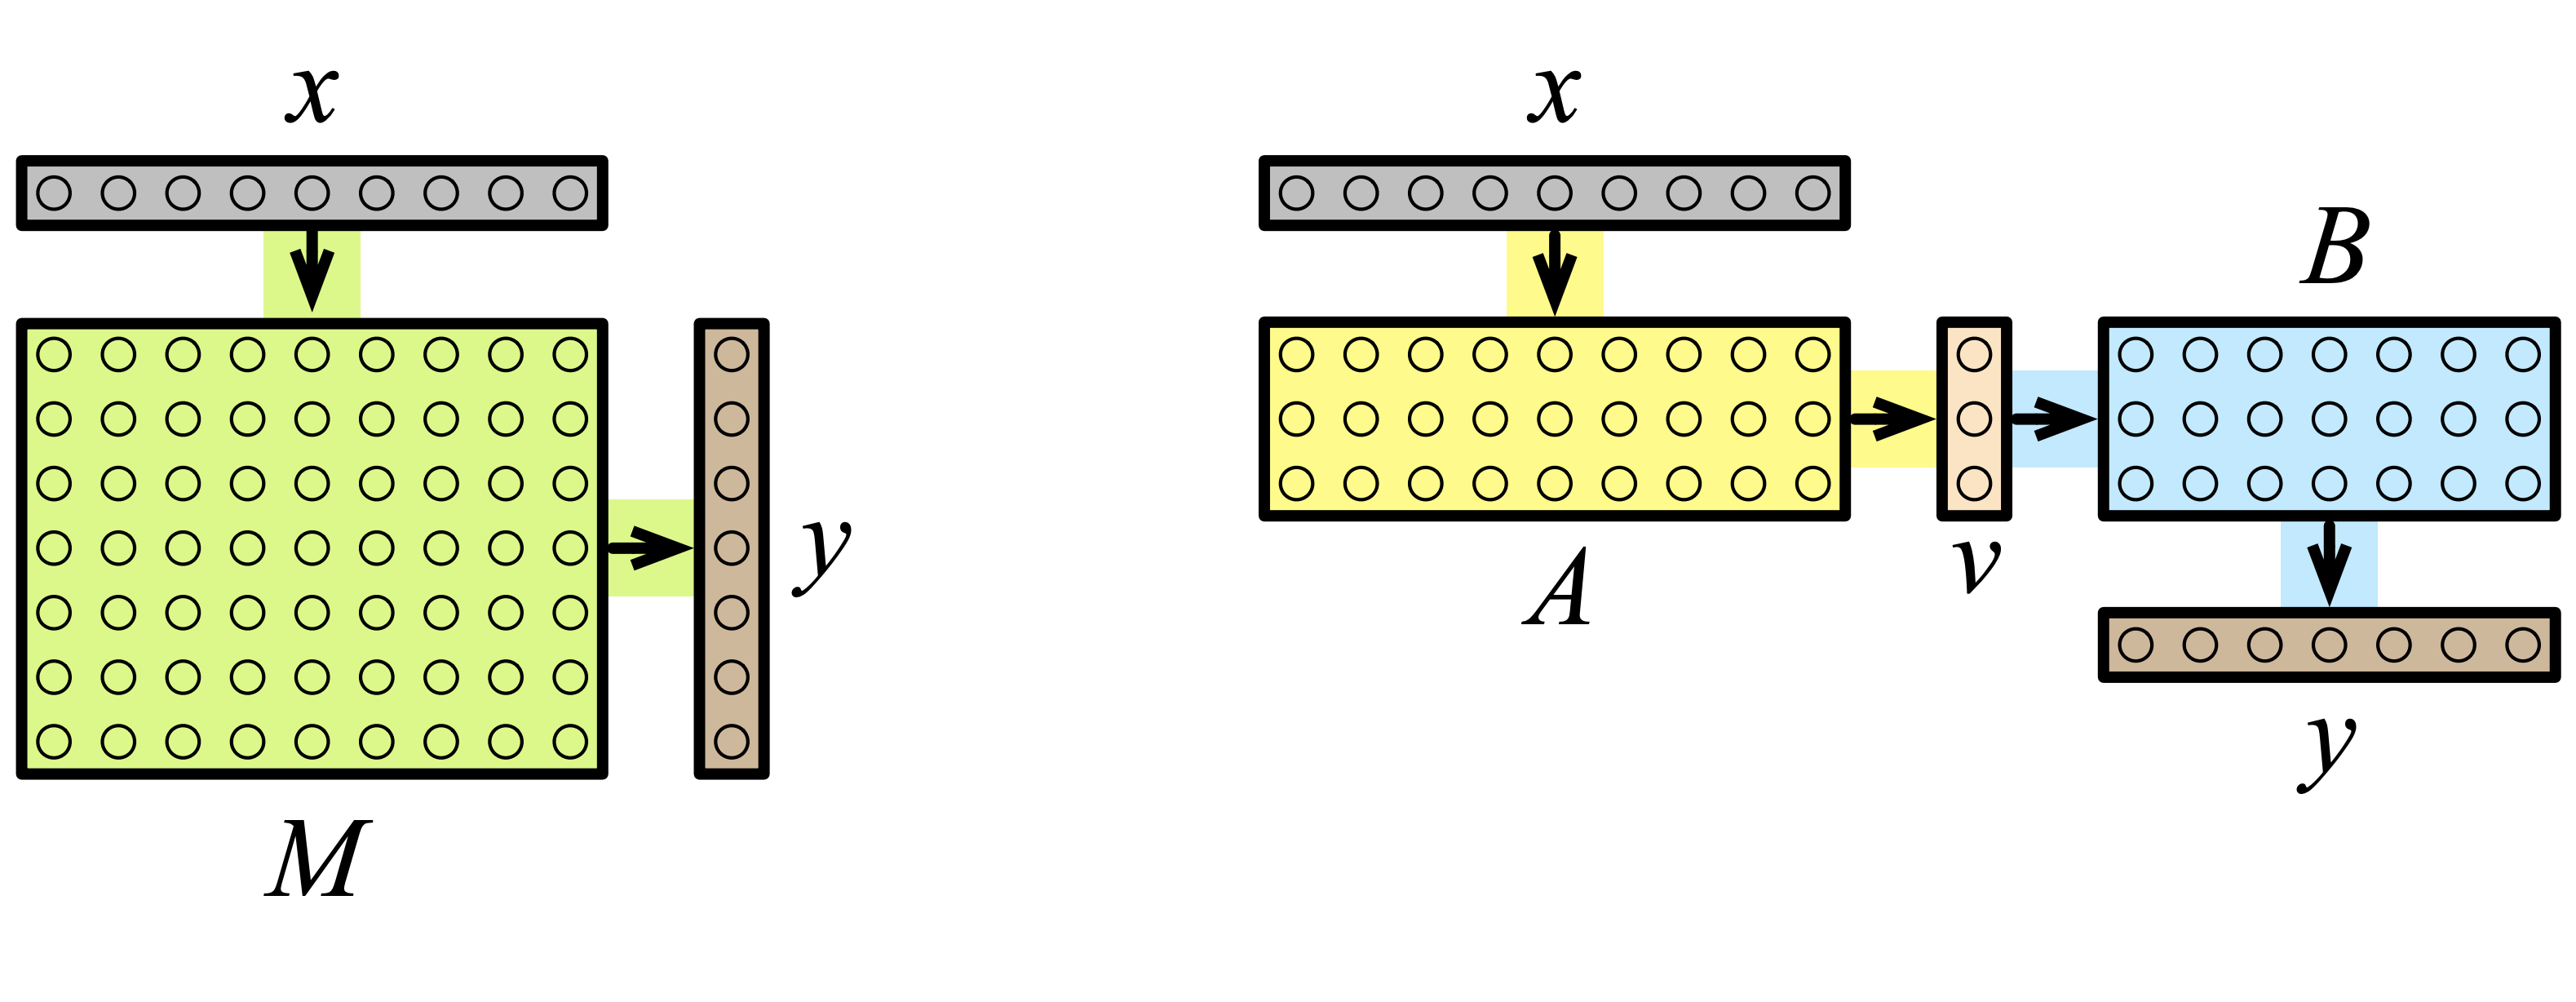
\includegraphics[width=10cm]{assets/factored_decomp}
\end{figure}
\begin{itemize}
  \item \textbf{Problem:} Large input and output vectors
  \begin{itemize}
    \item $|x| = 20,000$, $|y|=50,000$ $\rightarrow$ $|M|=1,000,000,000$
  \end{itemize}
  \item \textbf{Solution:} Use a bottleneck with smaller matrices $A$, $B$
  \begin{itemize}
    \item $|v| = 100$ $\rightarrow$ $|A|= 2,000,000$, $|B|= 5,000,000$
    \item Total Parameters: $7,000,000$
  \end{itemize}
\end{itemize}
\end{frame}


\begin{frame}
\frametitle{Character-Based Models}
\begin{itemize}
  \item Instead use embeddings for character string $\textcolor{ForestGreen}{\texttt{b e a u t i f u l}}$
  \item Idea is to induce embeddings for unseen morphological variants: $\textcolor{ForestGreen}{\texttt{beautiful}}$
  \item Tokens are single characters, symbols, whitespace
  \pause
  \item Generally poor performance
\end{itemize}
\end{frame}


\begin{frame}
  \frametitle{Character-Based Models}
  \begin{figure}
    \centering
    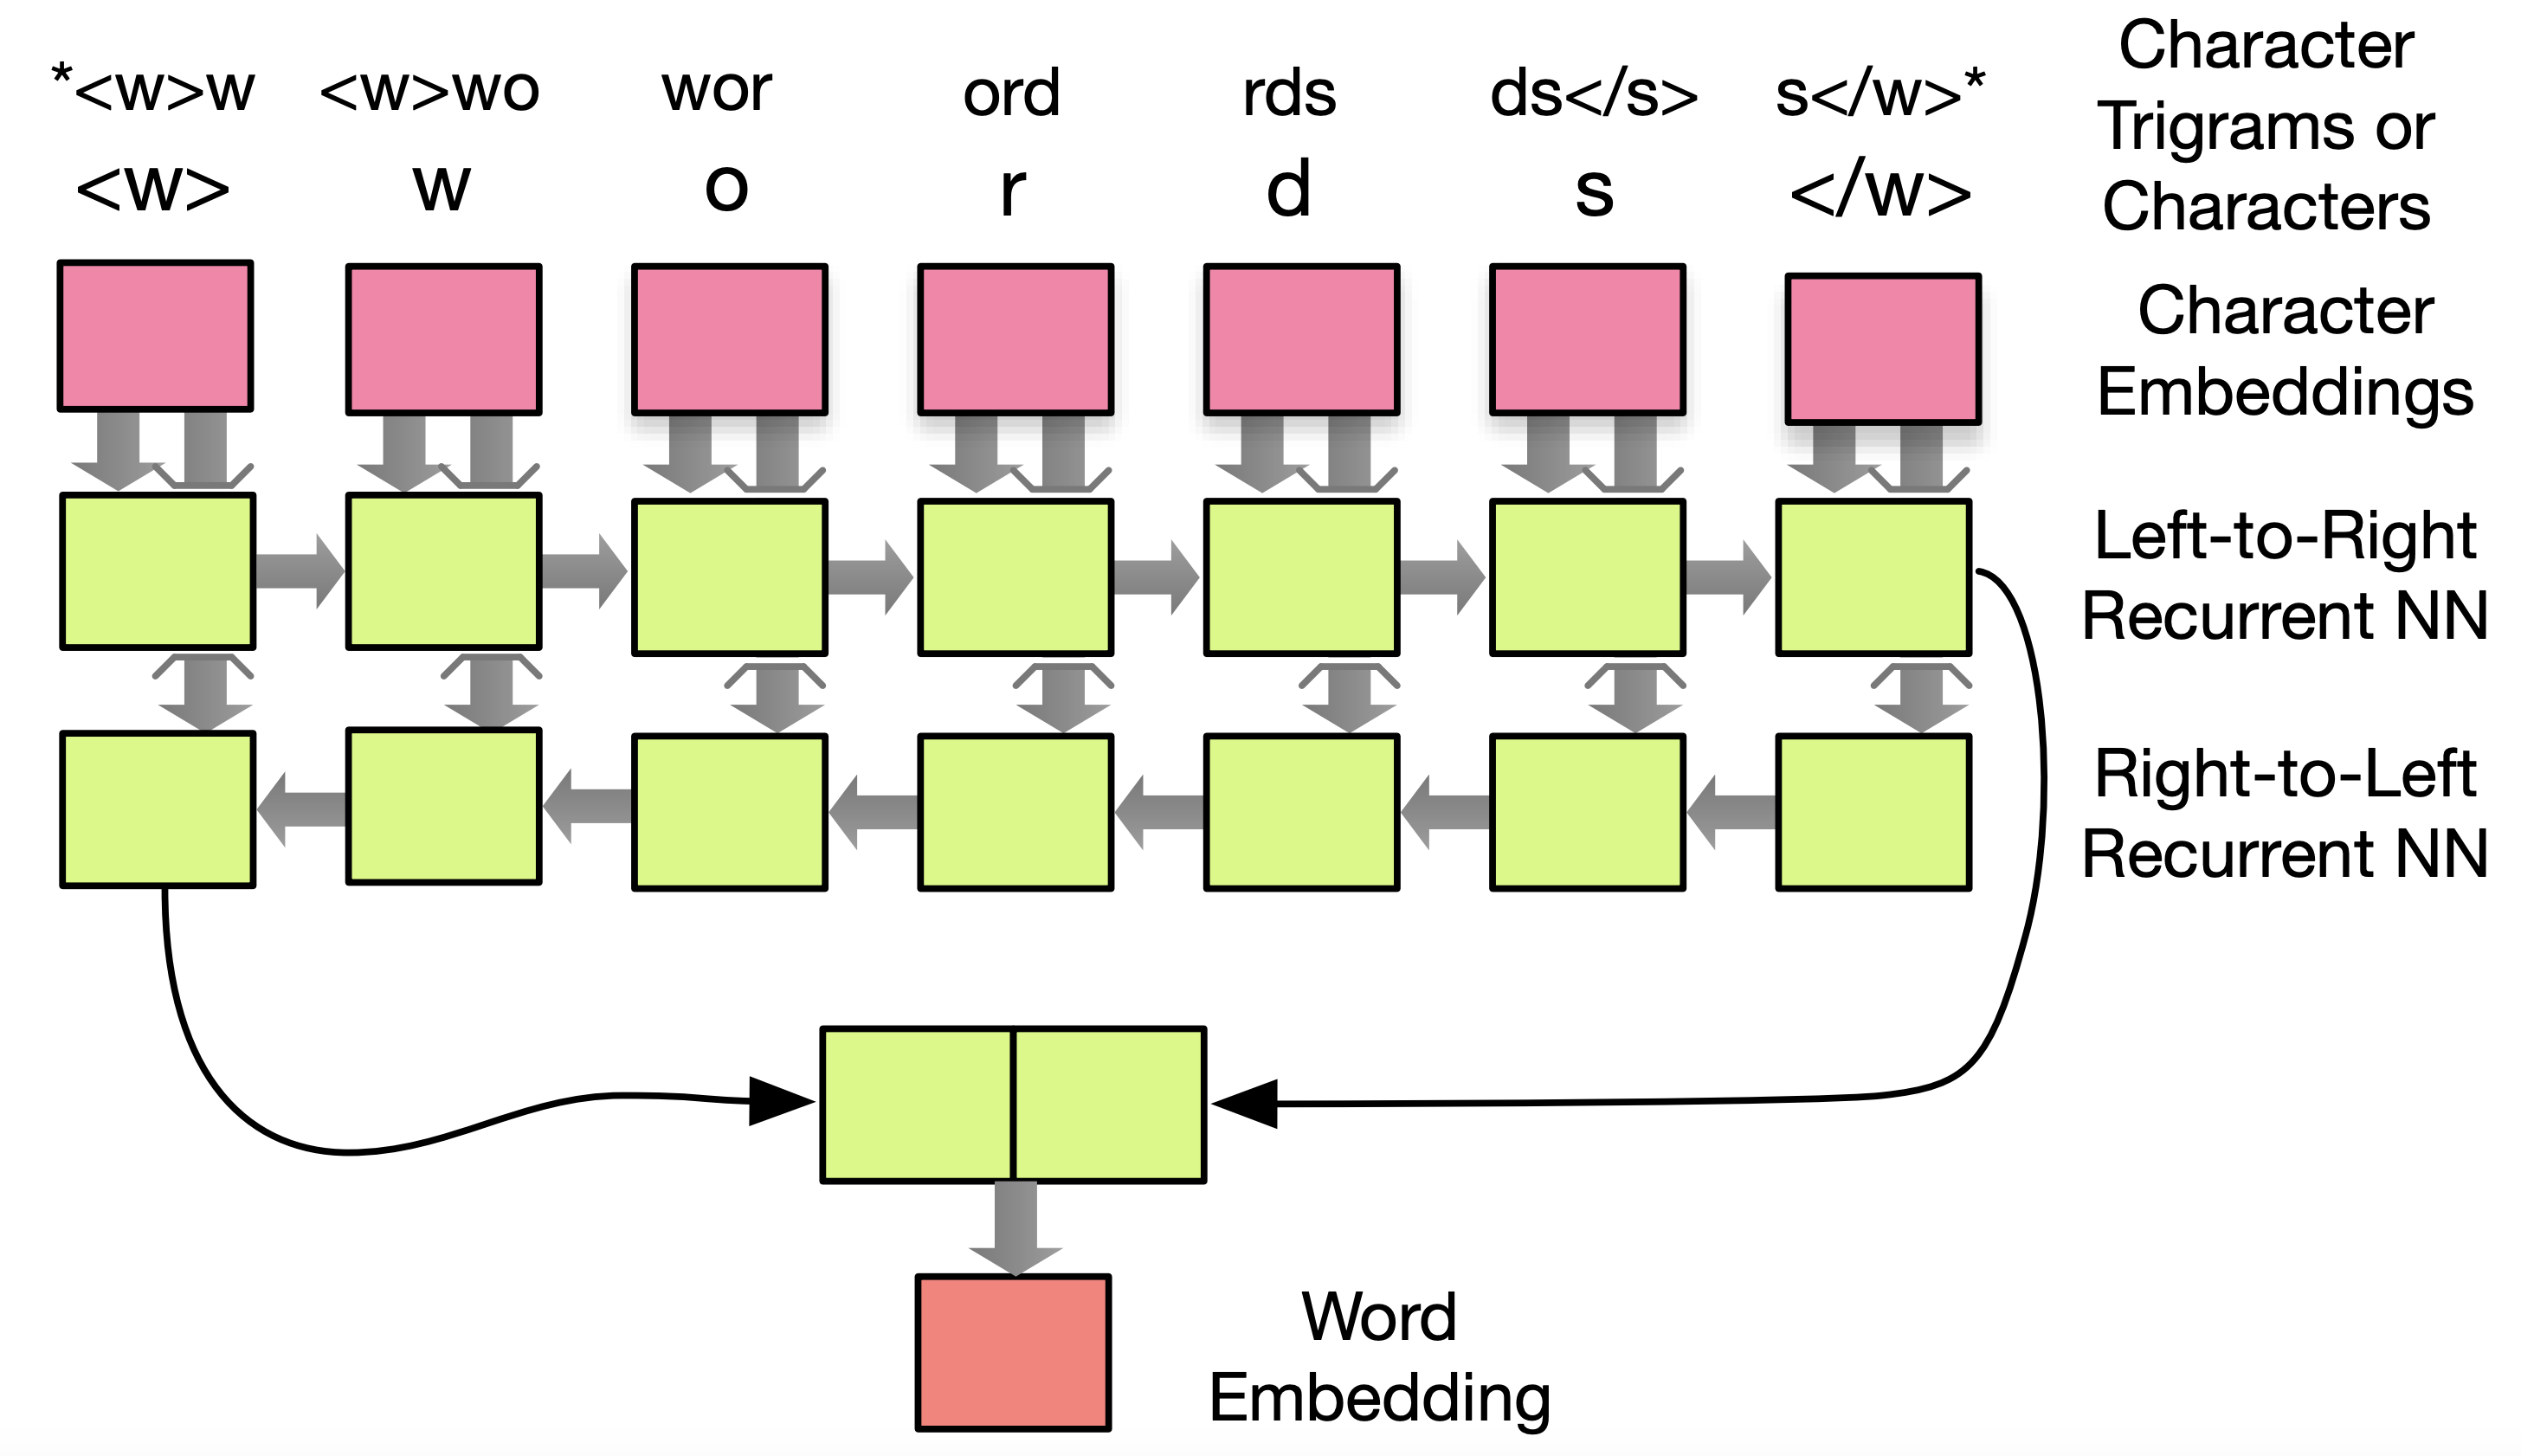
\includegraphics[height=6.5cm, valign=c]{assets/char_interpolate}
  \end{figure}
\end{frame}

\begin{frame}
  \frametitle{Character-Based Models}
  \begin{figure}
    \centering
    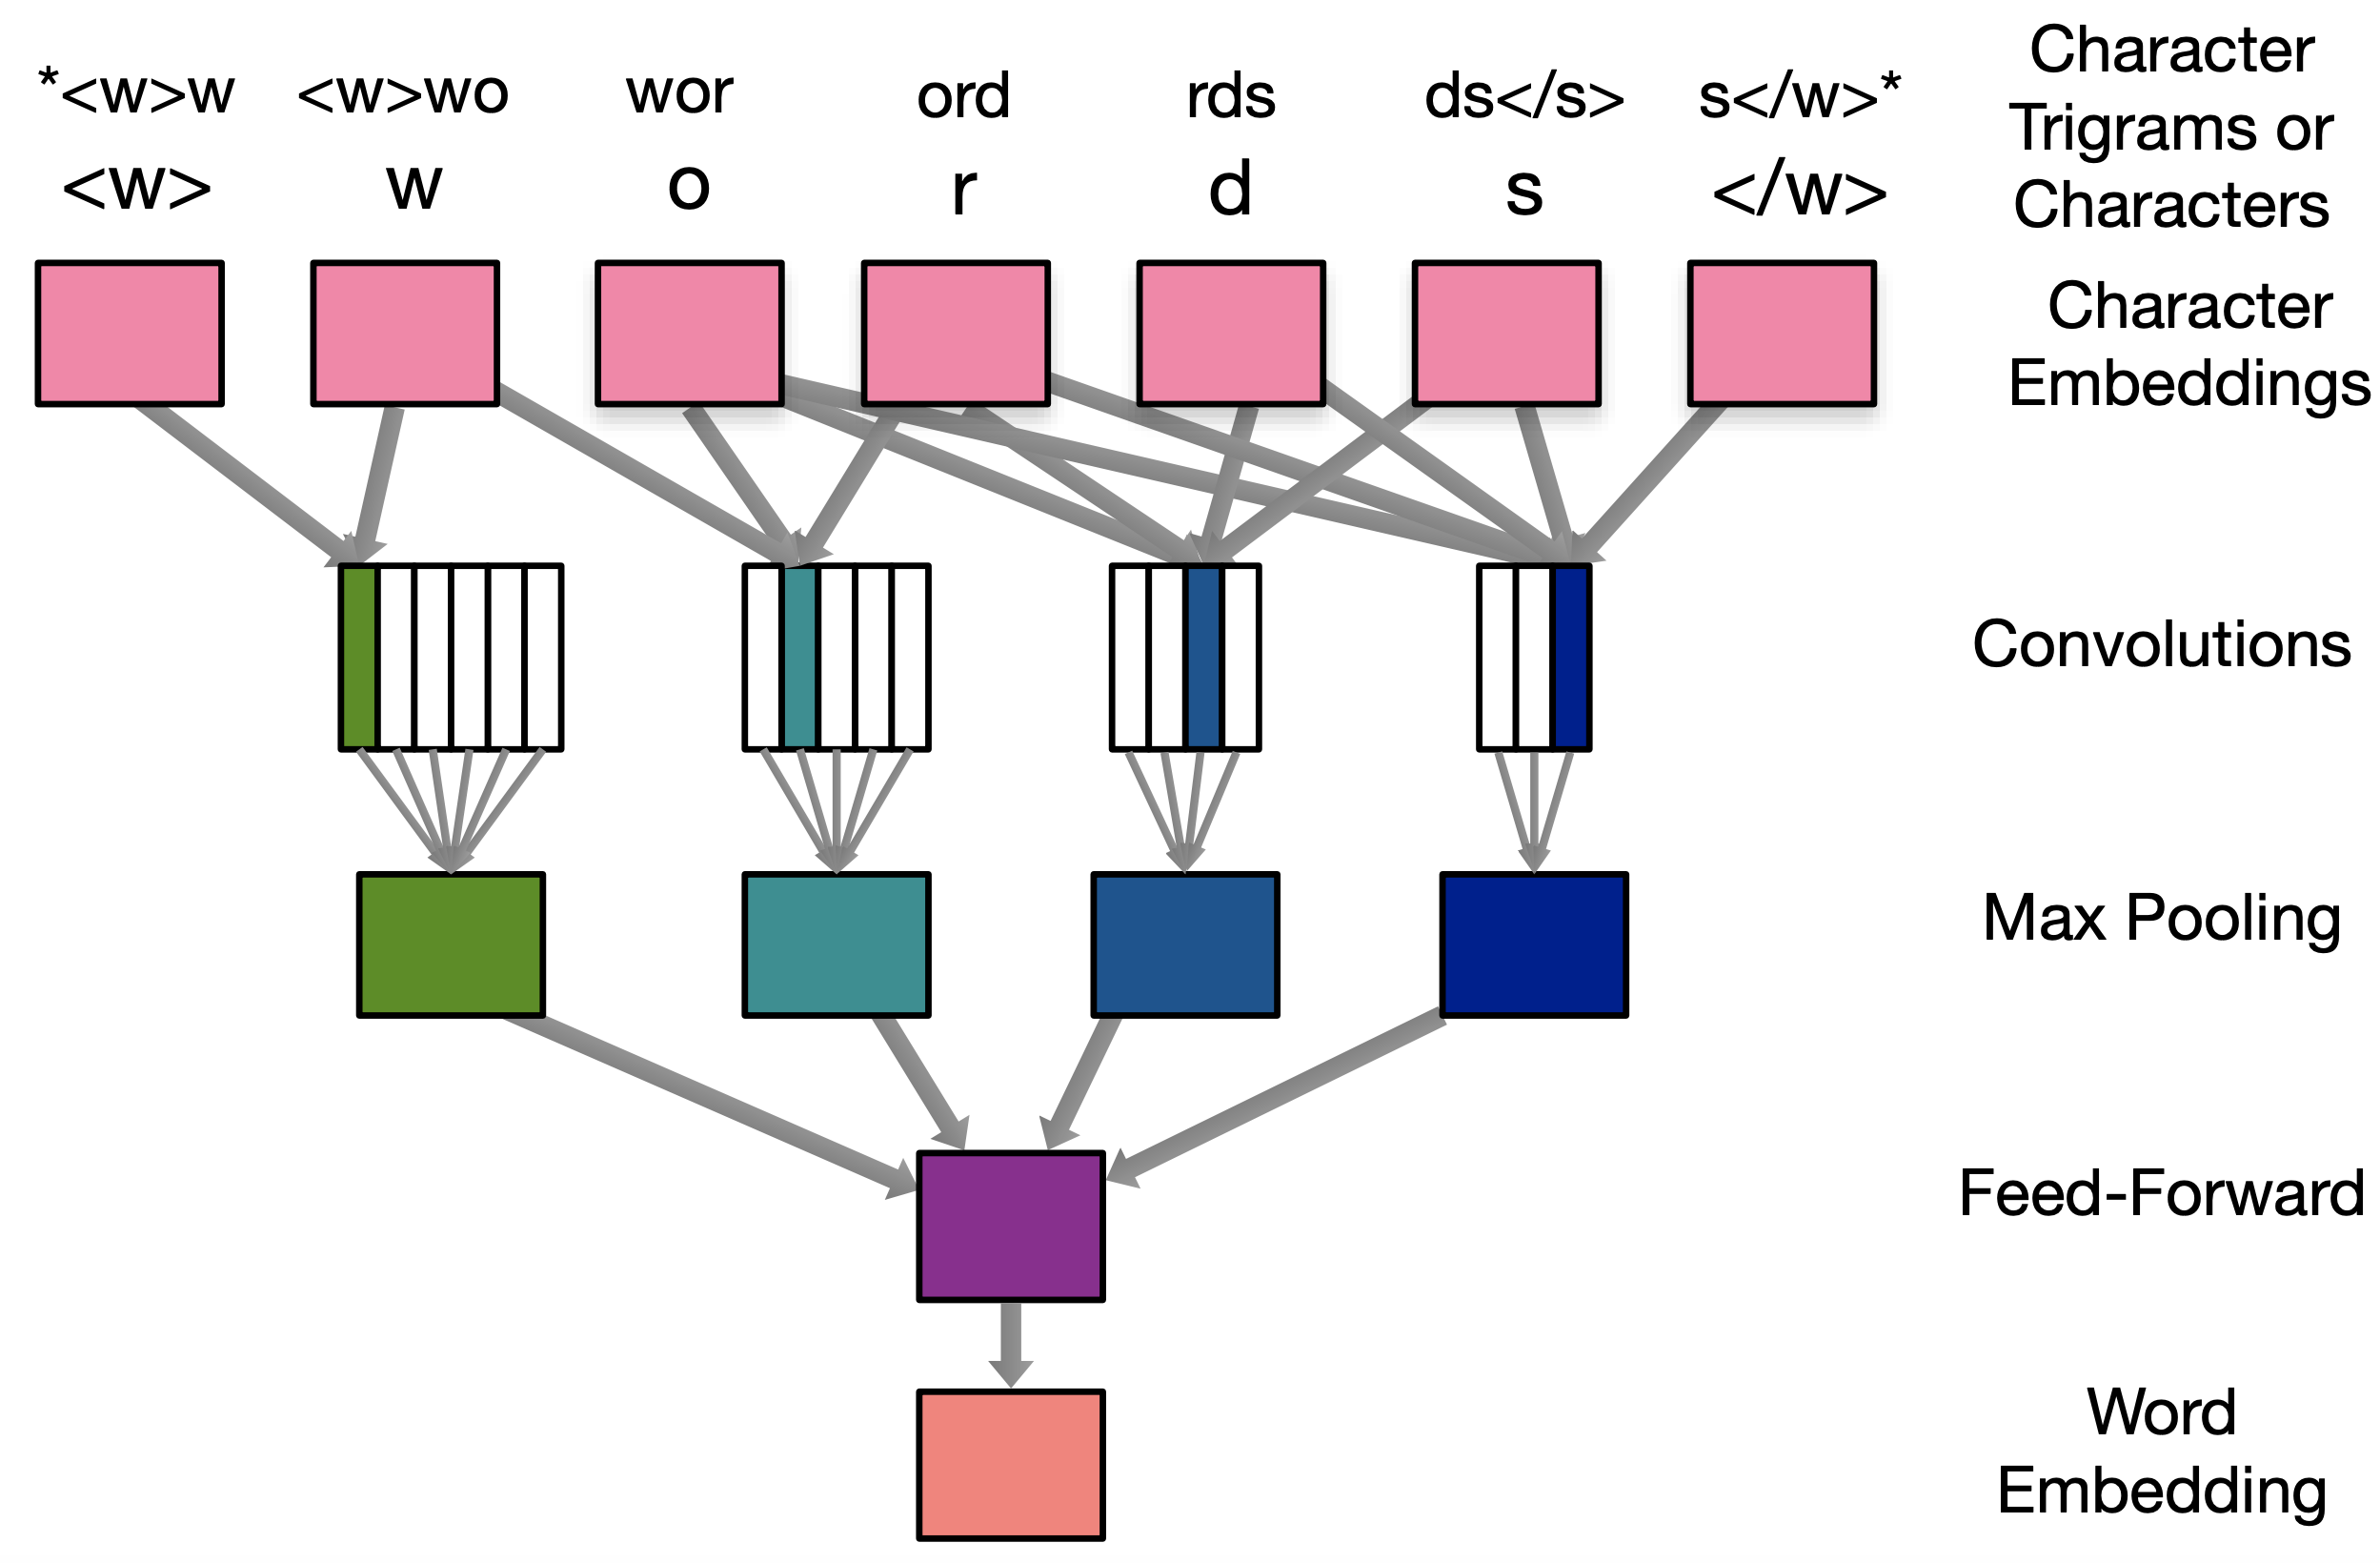
\includegraphics[height=6.5cm, valign=c]{assets/char_conv}
  \end{figure}
\end{frame}


\begin{frame}
\frametitle{BPE Subwords}
\footnotesize
\begin{equation*}
  \textcolor{ForestGreen}{\texttt{t h e $\cdotp$ f a t $\cdotp$ c a t $\cdotp$ i s $\cdotp$ i n $\cdotp$ t h e $\cdotp$ t h i n $\cdotp$ b a g}}
\end{equation*}
%\vspace{5mm}
\begin{equation*}
  \begin{array}{l l}
    \textcolor{ForestGreen}{\texttt{t h $\rightarrow$ th}} & \textcolor{ForestGreen}{\texttt{th e $\cdotp$ f a t $\cdotp$ c a t $\cdotp$ i s $\cdotp$ i n $\cdotp$ th e $\cdotp$ th i n $\cdotp$ b a g}} \\
    \textcolor{ForestGreen}{\texttt{a t $\rightarrow$ at}} & \textcolor{ForestGreen}{\texttt{th e $\cdotp$ f at $\cdotp$ c at $\cdotp$ i s $\cdotp$ i n $\cdotp$ th e $\cdotp$ th i n $\cdotp$ b a g}} \\
    \textcolor{ForestGreen}{\texttt{i n $\rightarrow$ in}} & \textcolor{ForestGreen}{\texttt{th e $\cdotp$ f at $\cdotp$ c at $\cdotp$ i s $\cdotp$ in $\cdotp$ th e $\cdotp$ th in $\cdotp$ b a g}} \\
    \textcolor{ForestGreen}{\texttt{th e $\rightarrow$ the}} & \textcolor{ForestGreen}{\texttt{the $\cdotp$ f at $\cdotp$ c at $\cdotp$ i s $\cdotp$ in $\cdotp$ the $\cdotp$ th in $\cdotp$ b a g}} \\
  \end{array}
\end{equation*}
\normalsize
\begin{itemize}
  \item Breaks words into subwords
  \begin{itemize}
    \item Starts with the character set
    \item Merges the most frequent pairs, one per iteration
  \end{itemize}
  \item Unsupervised (accidental) morphology (frequency suffixes)
\end{itemize}
\end{frame}


\begin{frame}
\frametitle{BPE Tokenization on HHGTTG}
\begin{itemize}
  \item Unique Characters: $101$
  \item Unique BPE Tokens (1K iterations): $1,093$
  \item Unique BPE Tokens (5K iterations): $4,817$
  \item Unique Tokens: $9,541$
\end{itemize}
\footnotesize
\begin{equation*}
\textcolor{ForestGreen}{
\begin{array}{l}
  \texttt{there is a the\textcolor{Fuchsia}{@@} ory which st\textcolor{Fuchsia}{@@} at\textcolor{Fuchsia}{@@} es that if ever any\textcolor{Fuchsia}{@@} one } \\
  \texttt{di\textcolor{Fuchsia}{@@} sc\textcolor{Fuchsia}{@@} o\textcolor{Fuchsia}{@@} ver\textcolor{Fuchsia}{@@} s ex\textcolor{Fuchsia}{@@} ac\textcolor{Fuchsia}{@@} tly what the universe is for } \\
  \texttt{and why it is here , it will in\textcolor{Fuchsia}{@@} stan\textcolor{Fuchsia}{@@} tly di\textcolor{Fuchsia}{@@} s\textcolor{Fuchsia}{@@} ap\textcolor{Fuchsia}{@@} pe\textcolor{Fuchsia}{@@} ar } \\
  \texttt{and be re\textcolor{Fuchsia}{@@} pl\textcolor{Fuchsia}{@@} ac\textcolor{Fuchsia}{@@} ed by something even more bi\textcolor{Fuchsia}{@@} zar\textcolor{Fuchsia}{@@} re } \\
  \texttt{and in\textcolor{Fuchsia}{@@} ex\textcolor{Fuchsia}{@@} p\textcolor{Fuchsia}{@@} li\textcolor{Fuchsia}{@@} c\textcolor{Fuchsia}{@@} able . } \\
  \texttt{there is another the\textcolor{Fuchsia}{@@} ory which st\textcolor{Fuchsia}{@@} at\textcolor{Fuchsia}{@@} es that } \\
  \texttt{this has al\textcolor{Fuchsia}{@@} re\textcolor{Fuchsia}{@@} ad\textcolor{Fuchsia}{@@} y happ\textcolor{Fuchsia}{@@} ened .} \\
  \texttt{in the beg\textcolor{Fuchsia}{@@} in\textcolor{Fuchsia}{@@} ning the universe was cre\textcolor{Fuchsia}{@@} ated . } \\
  \texttt{this has made a lot of people very an\textcolor{Fuchsia}{@@} gr\textcolor{Fuchsia}{@@} y and } \\
  \texttt{been wi\textcolor{Fuchsia}{@@} de\textcolor{Fuchsia}{@@} ly re\textcolor{Fuchsia}{@@} gar\textcolor{Fuchsia}{@@} ded as a b\textcolor{Fuchsia}{@@} ad mo\textcolor{Fuchsia}{@@} ve .}
  %
  % \texttt{it was the b\textcolor{Fuchsia}{@@} est of times ,} \\
  % \texttt{it was the wor\textcolor{Fuchsia}{@@} st of times ,} \\
  % \texttt{it was the age of w\textcolor{Fuchsia}{@@} is\textcolor{Fuchsia}{@@} do\textcolor{Fuchsia}{@@} m ,} \\
  % \texttt{it was the age of foo\textcolor{Fuchsia}{@@} li\textcolor{Fuchsia}{@@} sh\textcolor{Fuchsia}{@@} ness ,} \\
  % \texttt{it was the e\textcolor{Fuchsia}{@@} po\textcolor{Fuchsia}{@@} ch of beli\textcolor{Fuchsia}{@@} e\textcolor{Fuchsia}{@@} f ,} \\
  % \texttt{it was the e\textcolor{Fuchsia}{@@} po\textcolor{Fuchsia}{@@} ch of in\textcolor{Fuchsia}{@@} cre\textcolor{Fuchsia}{@@} du\textcolor{Fuchsia}{@@} l\textcolor{Fuchsia}{@@} ity ,} \\
  % \texttt{it was the s\textcolor{Fuchsia}{@@} ea\textcolor{Fuchsia}{@@} son of light ,} \\
  % \texttt{it was the s\textcolor{Fuchsia}{@@} ea\textcolor{Fuchsia}{@@} son of dar\textcolor{Fuchsia}{@@} k\textcolor{Fuchsia}{@@} ness ,} \\
  % \texttt{it was the sp\textcolor{Fuchsia}{@@} r\textcolor{Fuchsia}{@@} ing of hope ,} \\
  % \texttt{it was the win\textcolor{Fuchsia}{@@} ter of des\textcolor{Fuchsia}{@@} pa\textcolor{Fuchsia}{@@} ir} \\
\end{array}}
\end{equation*}
\end{frame}

%%%%%%%%%%%%%%%%%%%%%%%%%%%%%%%%%%%%%%%%%%%%%%%%%%%%%%%%%%%%%%%%%%%%%%%%%%%%%%%%

\section{Column Segmentation Architecture}

\begin{frame}
  \frametitle{Seq2Seq Architecture}
  \begin{figure}
    \centering
    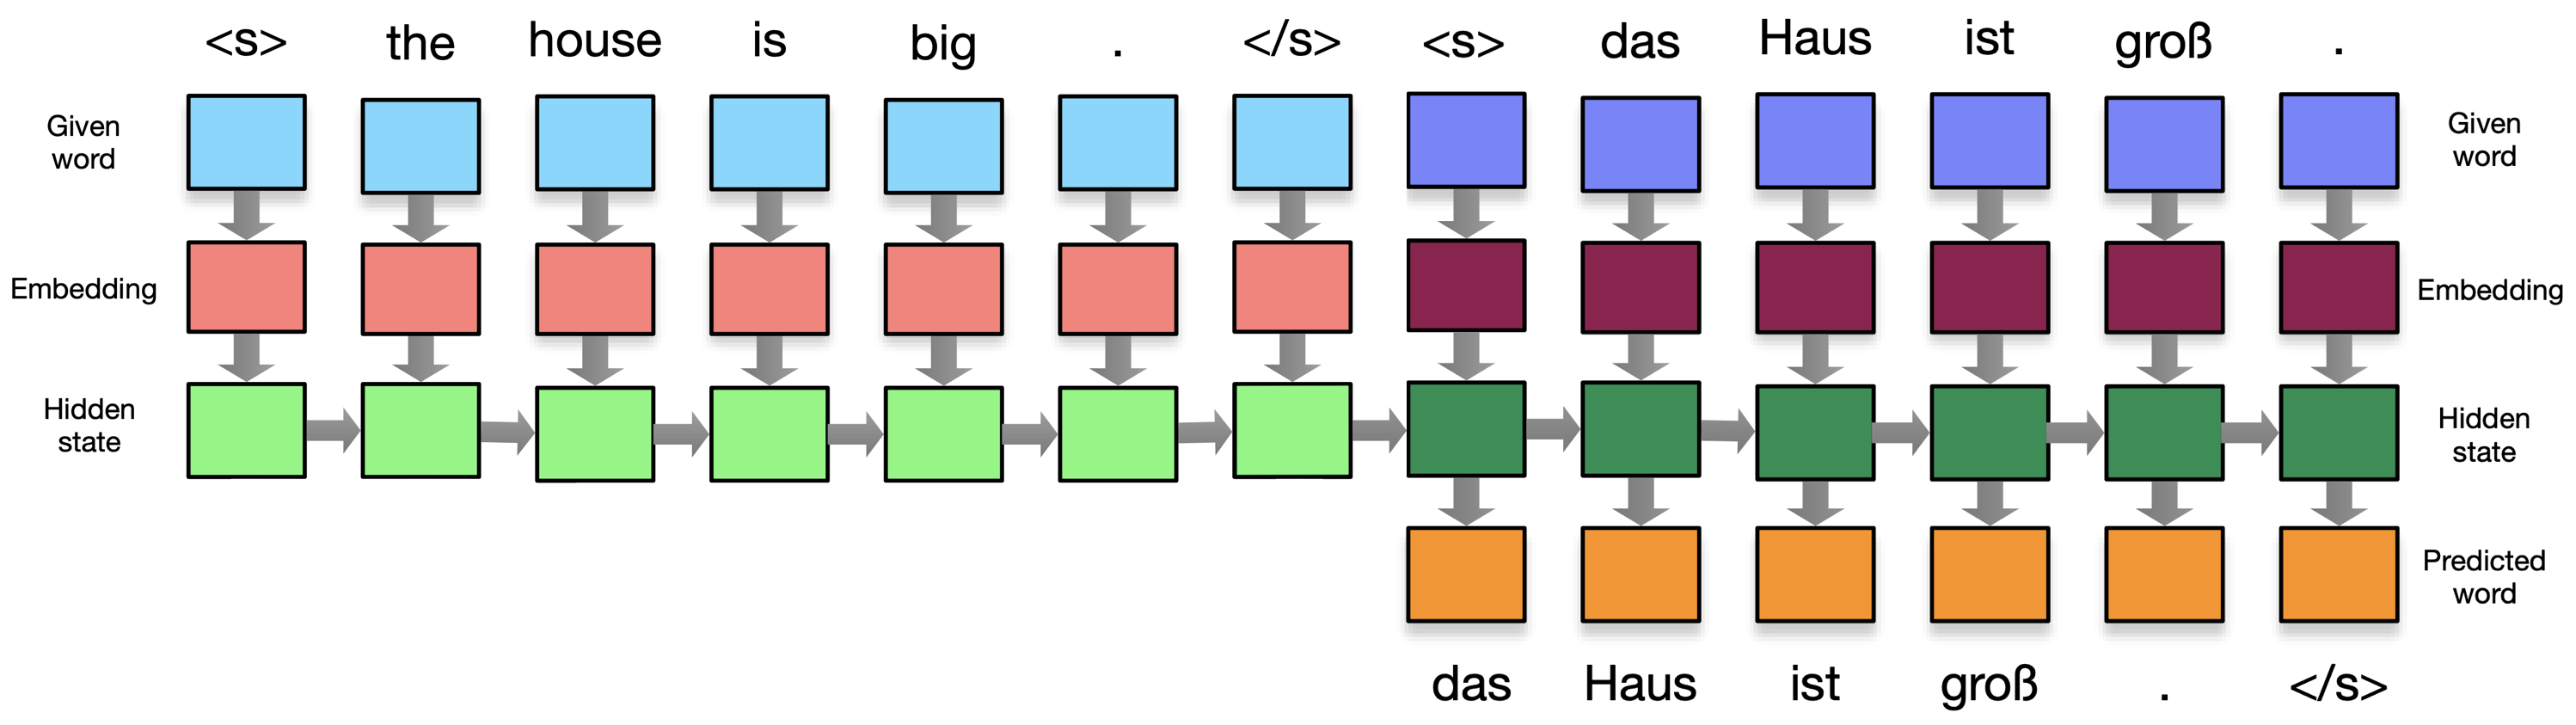
\includegraphics[width=10cm, valign=c]{assets/enc-dec}
  \end{figure}
  % add picture from notebook
  \begin{figure}
    \centering
    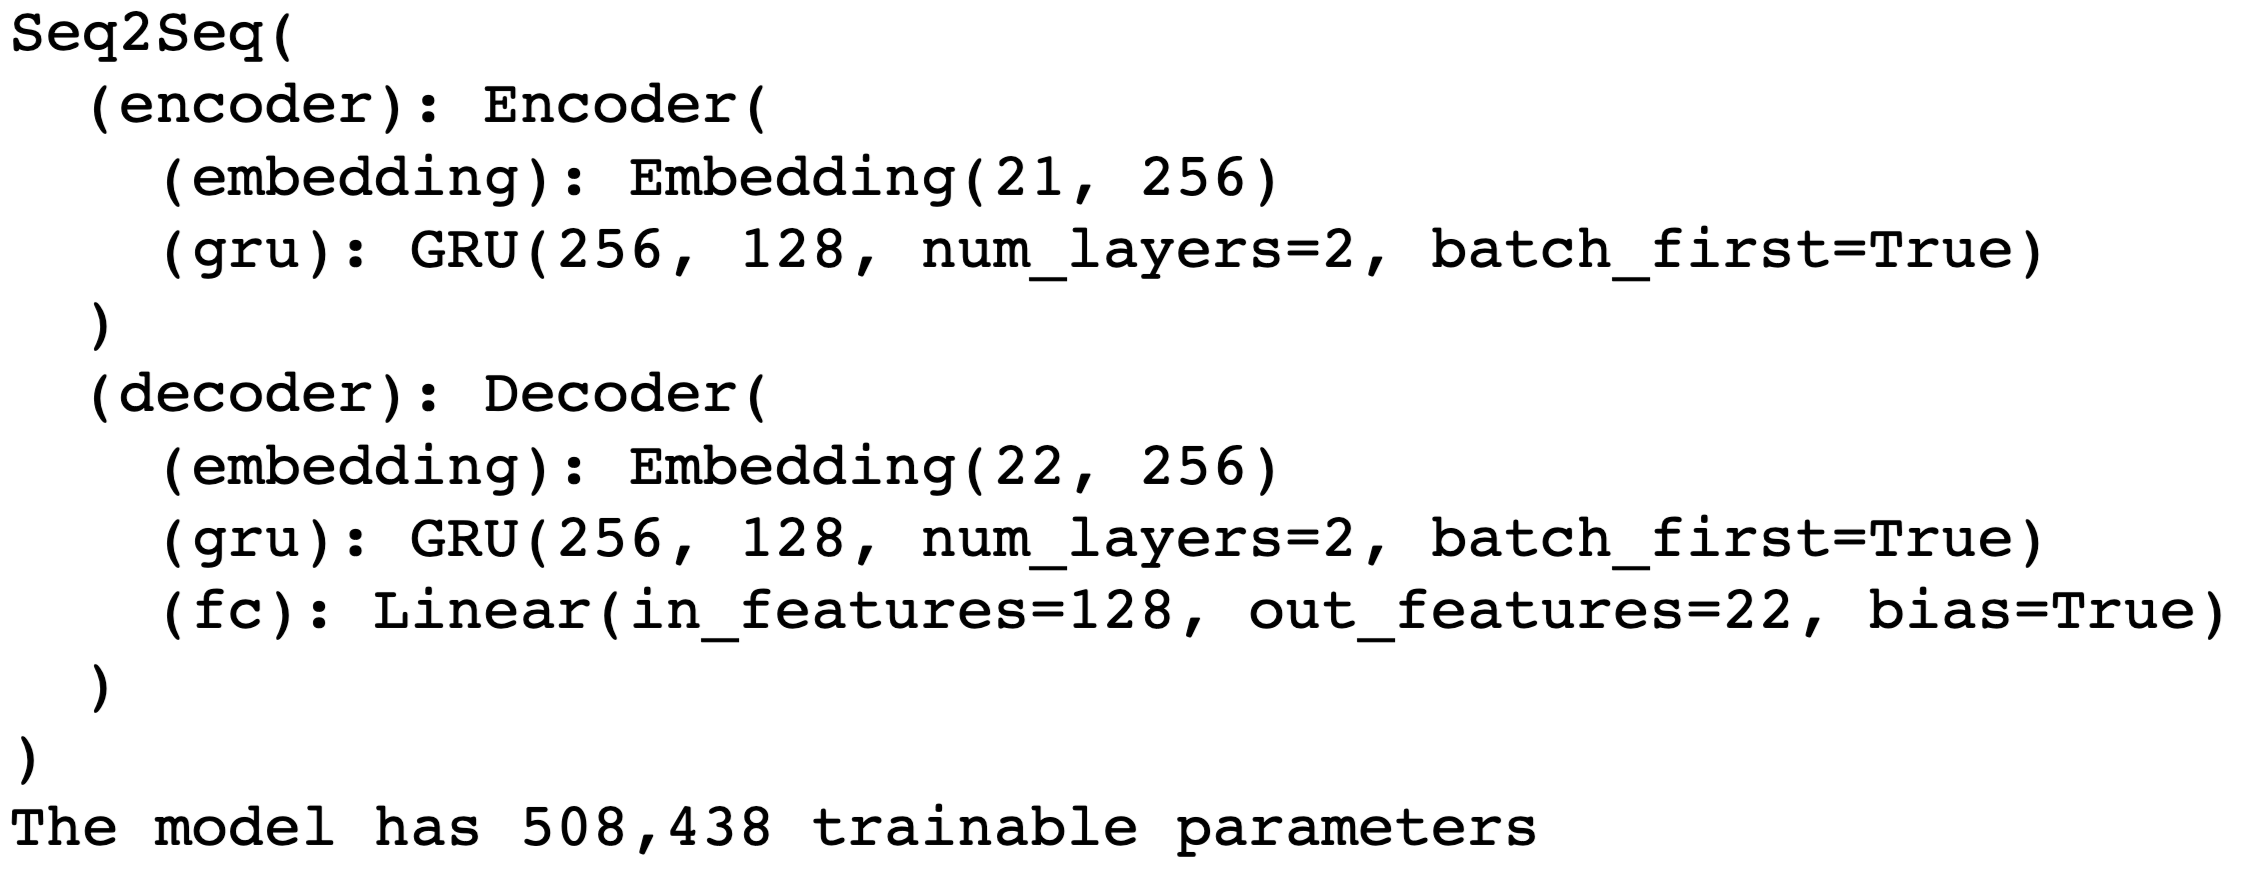
\includegraphics[width=10cm, valign=c]{assets/col-seq2seq}
  \end{figure}
\end{frame}


%%%%%%%%%%%%%%%%%%%%%%%%%%%%%%%%%%%%%%%%%%%%%%%%%%%%%%%%%%%%%%%%%%%%%%%%%%%%%%%%
\section{Training Considerations}

\begin{frame}
\frametitle{Increasing Throughput through Batching}
\begin{figure}
  \centering
  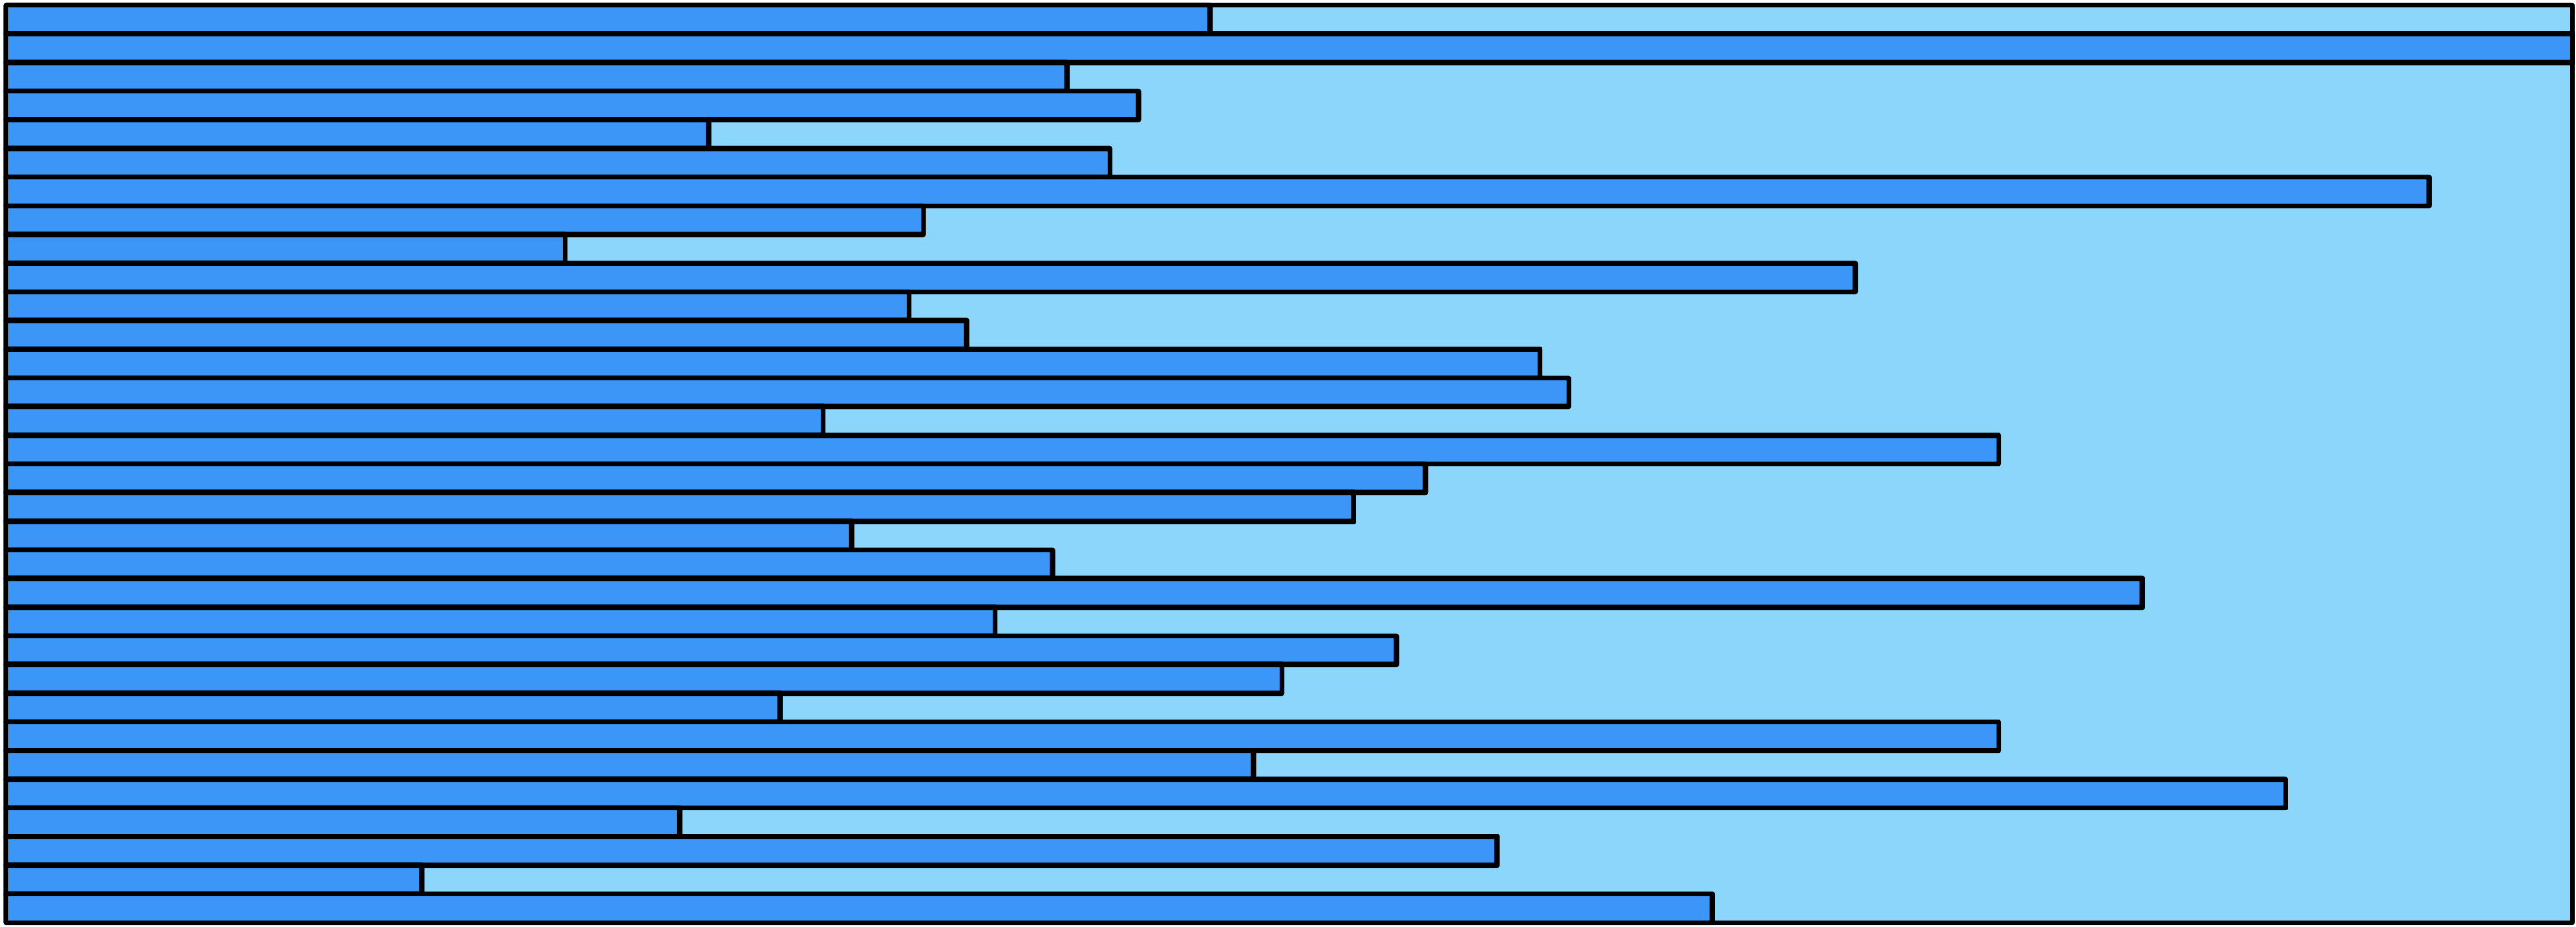
\includegraphics[width=4.5cm, valign=c]{assets/full_batch}
  \quad
  $\Longrightarrow$
  \quad
  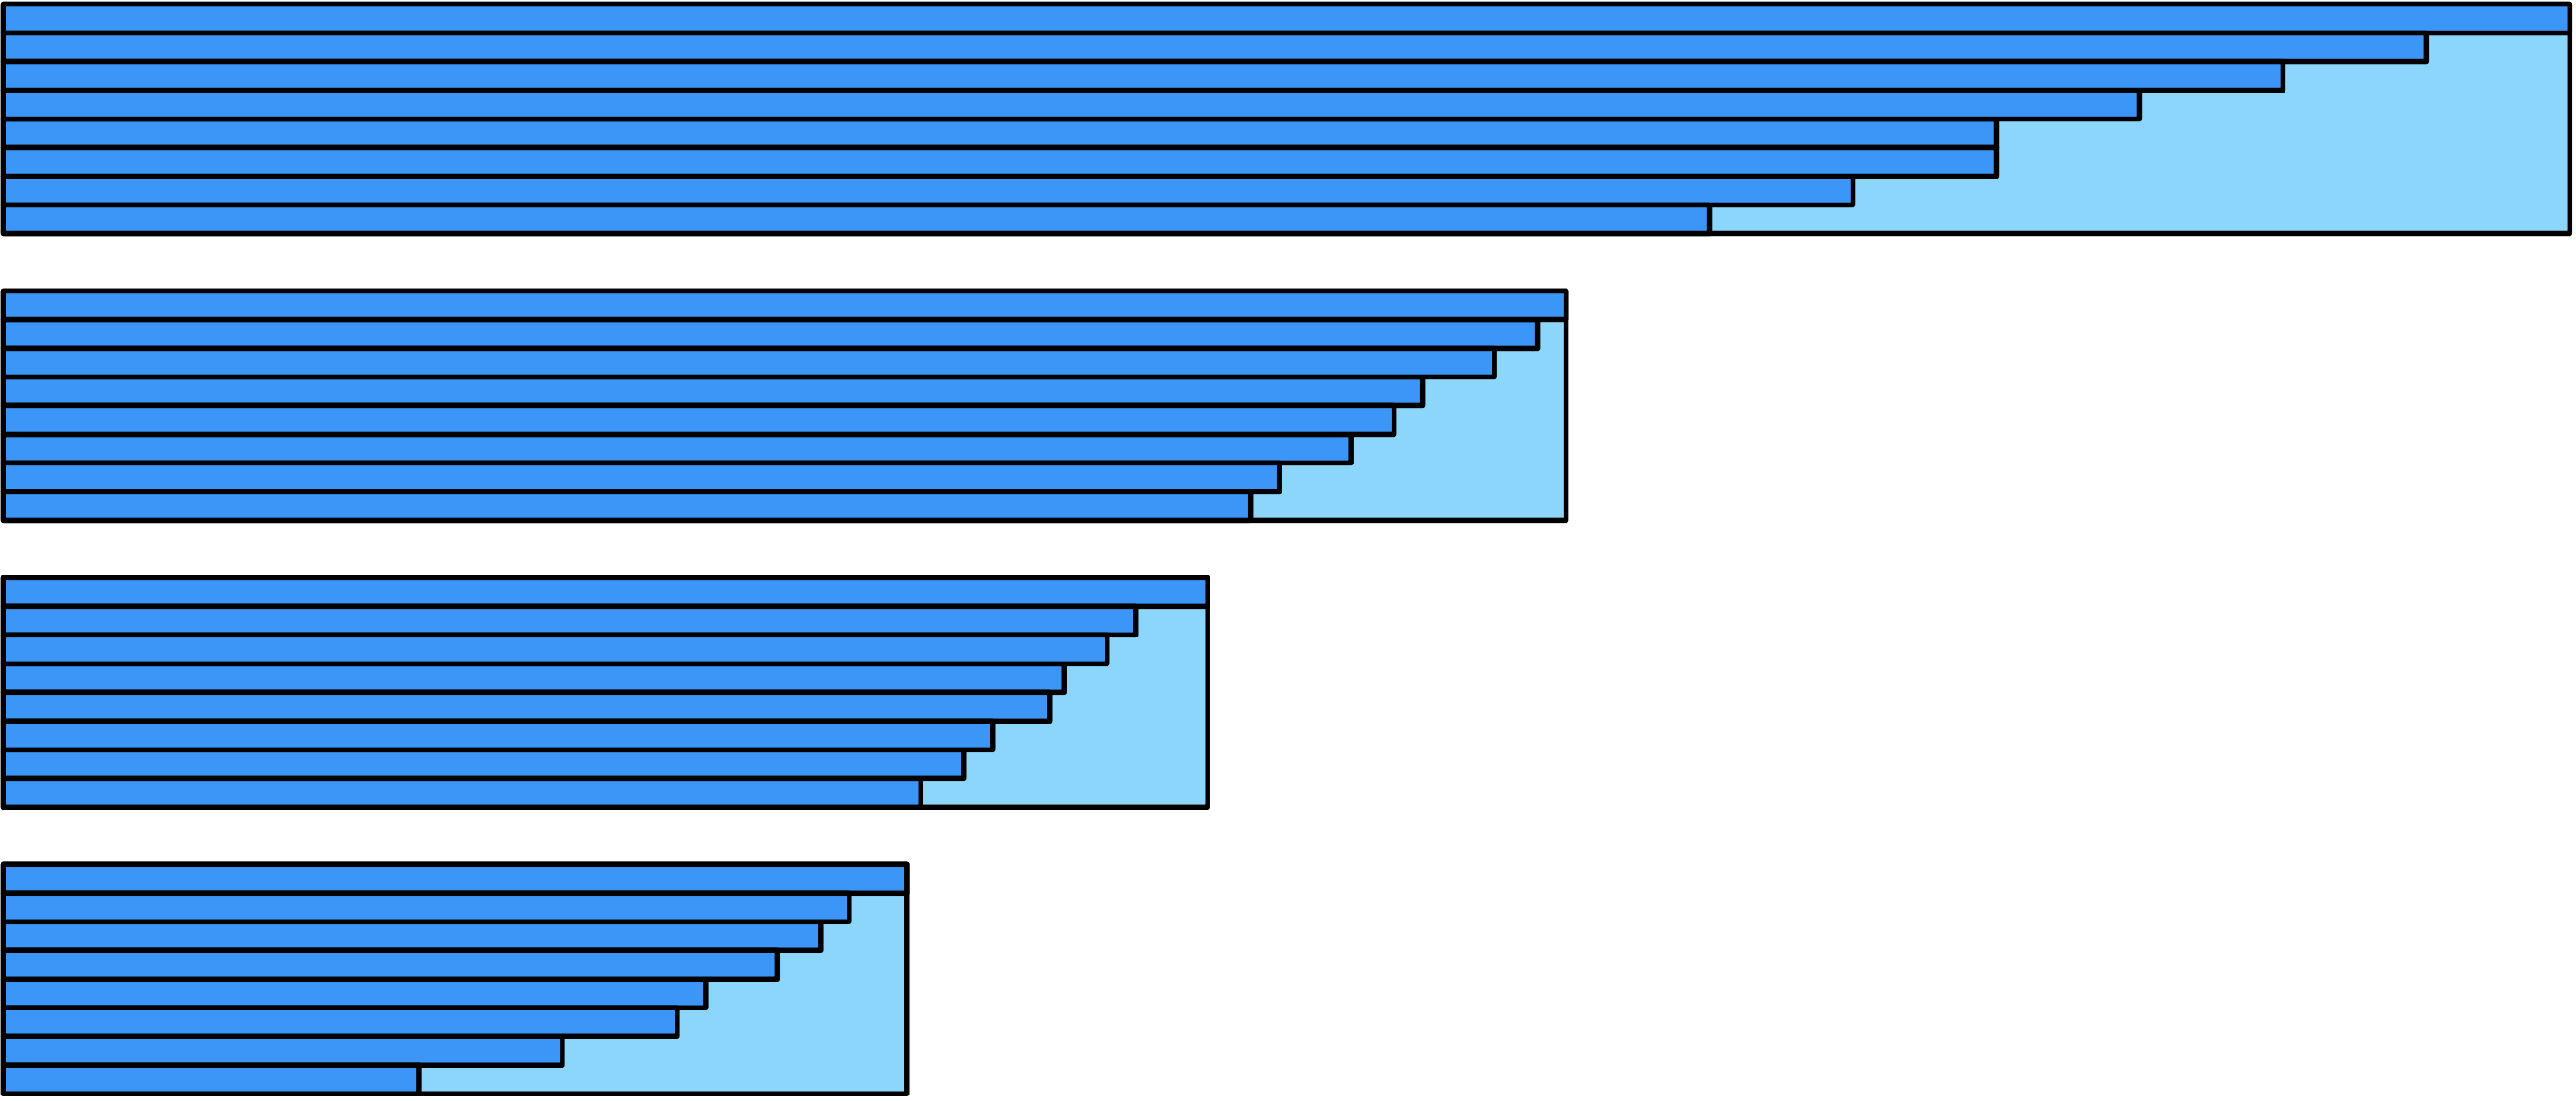
\includegraphics[width=4.5cm, valign=c]{assets/mini_batch}
\end{figure}
\begin{itemize}
  \item We can pad sentences of different lengths to increase batch size
  \item While also minimizing the use of padding
  \item Matrix Operations are faster
  \item \textbf{Warning!} Make sure padding is not influencing the hidden state
\end{itemize}
\end{frame}

\begin{frame}
\frametitle{Teacher Forcing}
\begin{itemize}
  \item Instead of refeeding the predicted token, replace it with the true token randomly
  \item This is only done during training, not inference
\end{itemize}
\begin{equation*}
  y_{i+1} = \begin{cases}
    \argmax_{j} \theta_i  & \mathcal{U}(0, 1) < \text{TF} \\
    t_{i+1} & else
  \end{cases}
\end{equation*}
\begin{itemize}
  \item $t_{i+1}$ is the true token
  \item $\text{TF}$ is the teacher forcing ratio
\end{itemize}
\end{frame}


\begin{frame}
\frametitle{Cross Entropy and Label Smoothing}
\begin{equation*}
  \begin{split}
    \ell\left(\mathbf{x}, y_i\right) =& - \log \left( \frac{\exp x_{y_i} }{\sum_j \exp x_j} \right) \\
    =& -\underbrace{x_{y_i}}_{max} + \underbrace{\log \sum_j \exp x_j}_{min}
  \end{split}
\end{equation*}
\begin{itemize}
  \item Softmax and Cross-Entropy loss assign all the probability mass to a single word
  \begin{itemize}
    \item LogSumExp is minimized on confident predictions
  \end{itemize}
  \item Solution: \textbf{smooth} the distribution
\end{itemize}
\end{frame}


\begin{frame}
\frametitle{Cross Entropy and Label Smoothing}
\begin{itemize}
  \item Softmax
  \begin{equation*}
    p(y_i) = \frac{\exp x_{y_i}}{\sum_j \exp x_j}
  \end{equation*}
  \item Smoothed Softmax with Temperature $T$
  \begin{equation*}
    p(y_i) = \frac{\exp \left(x_{y_i} / T \right)}{\sum_j \exp \left(x_j / T \right)}
  \end{equation*}
  \item As $T \to \infty$, the distribution is smoother, uniform
  \item AS $T \to 0$, the distribution approaches a kronecker delta centered on the class with the most mass
  \item \textbf{Question:} Why do we divide instead of adding/subtracting?
\end{itemize}
\end{frame}

\begin{frame}
\frametitle{Visualizing Temperature}
\begin{figure}
  \centering
  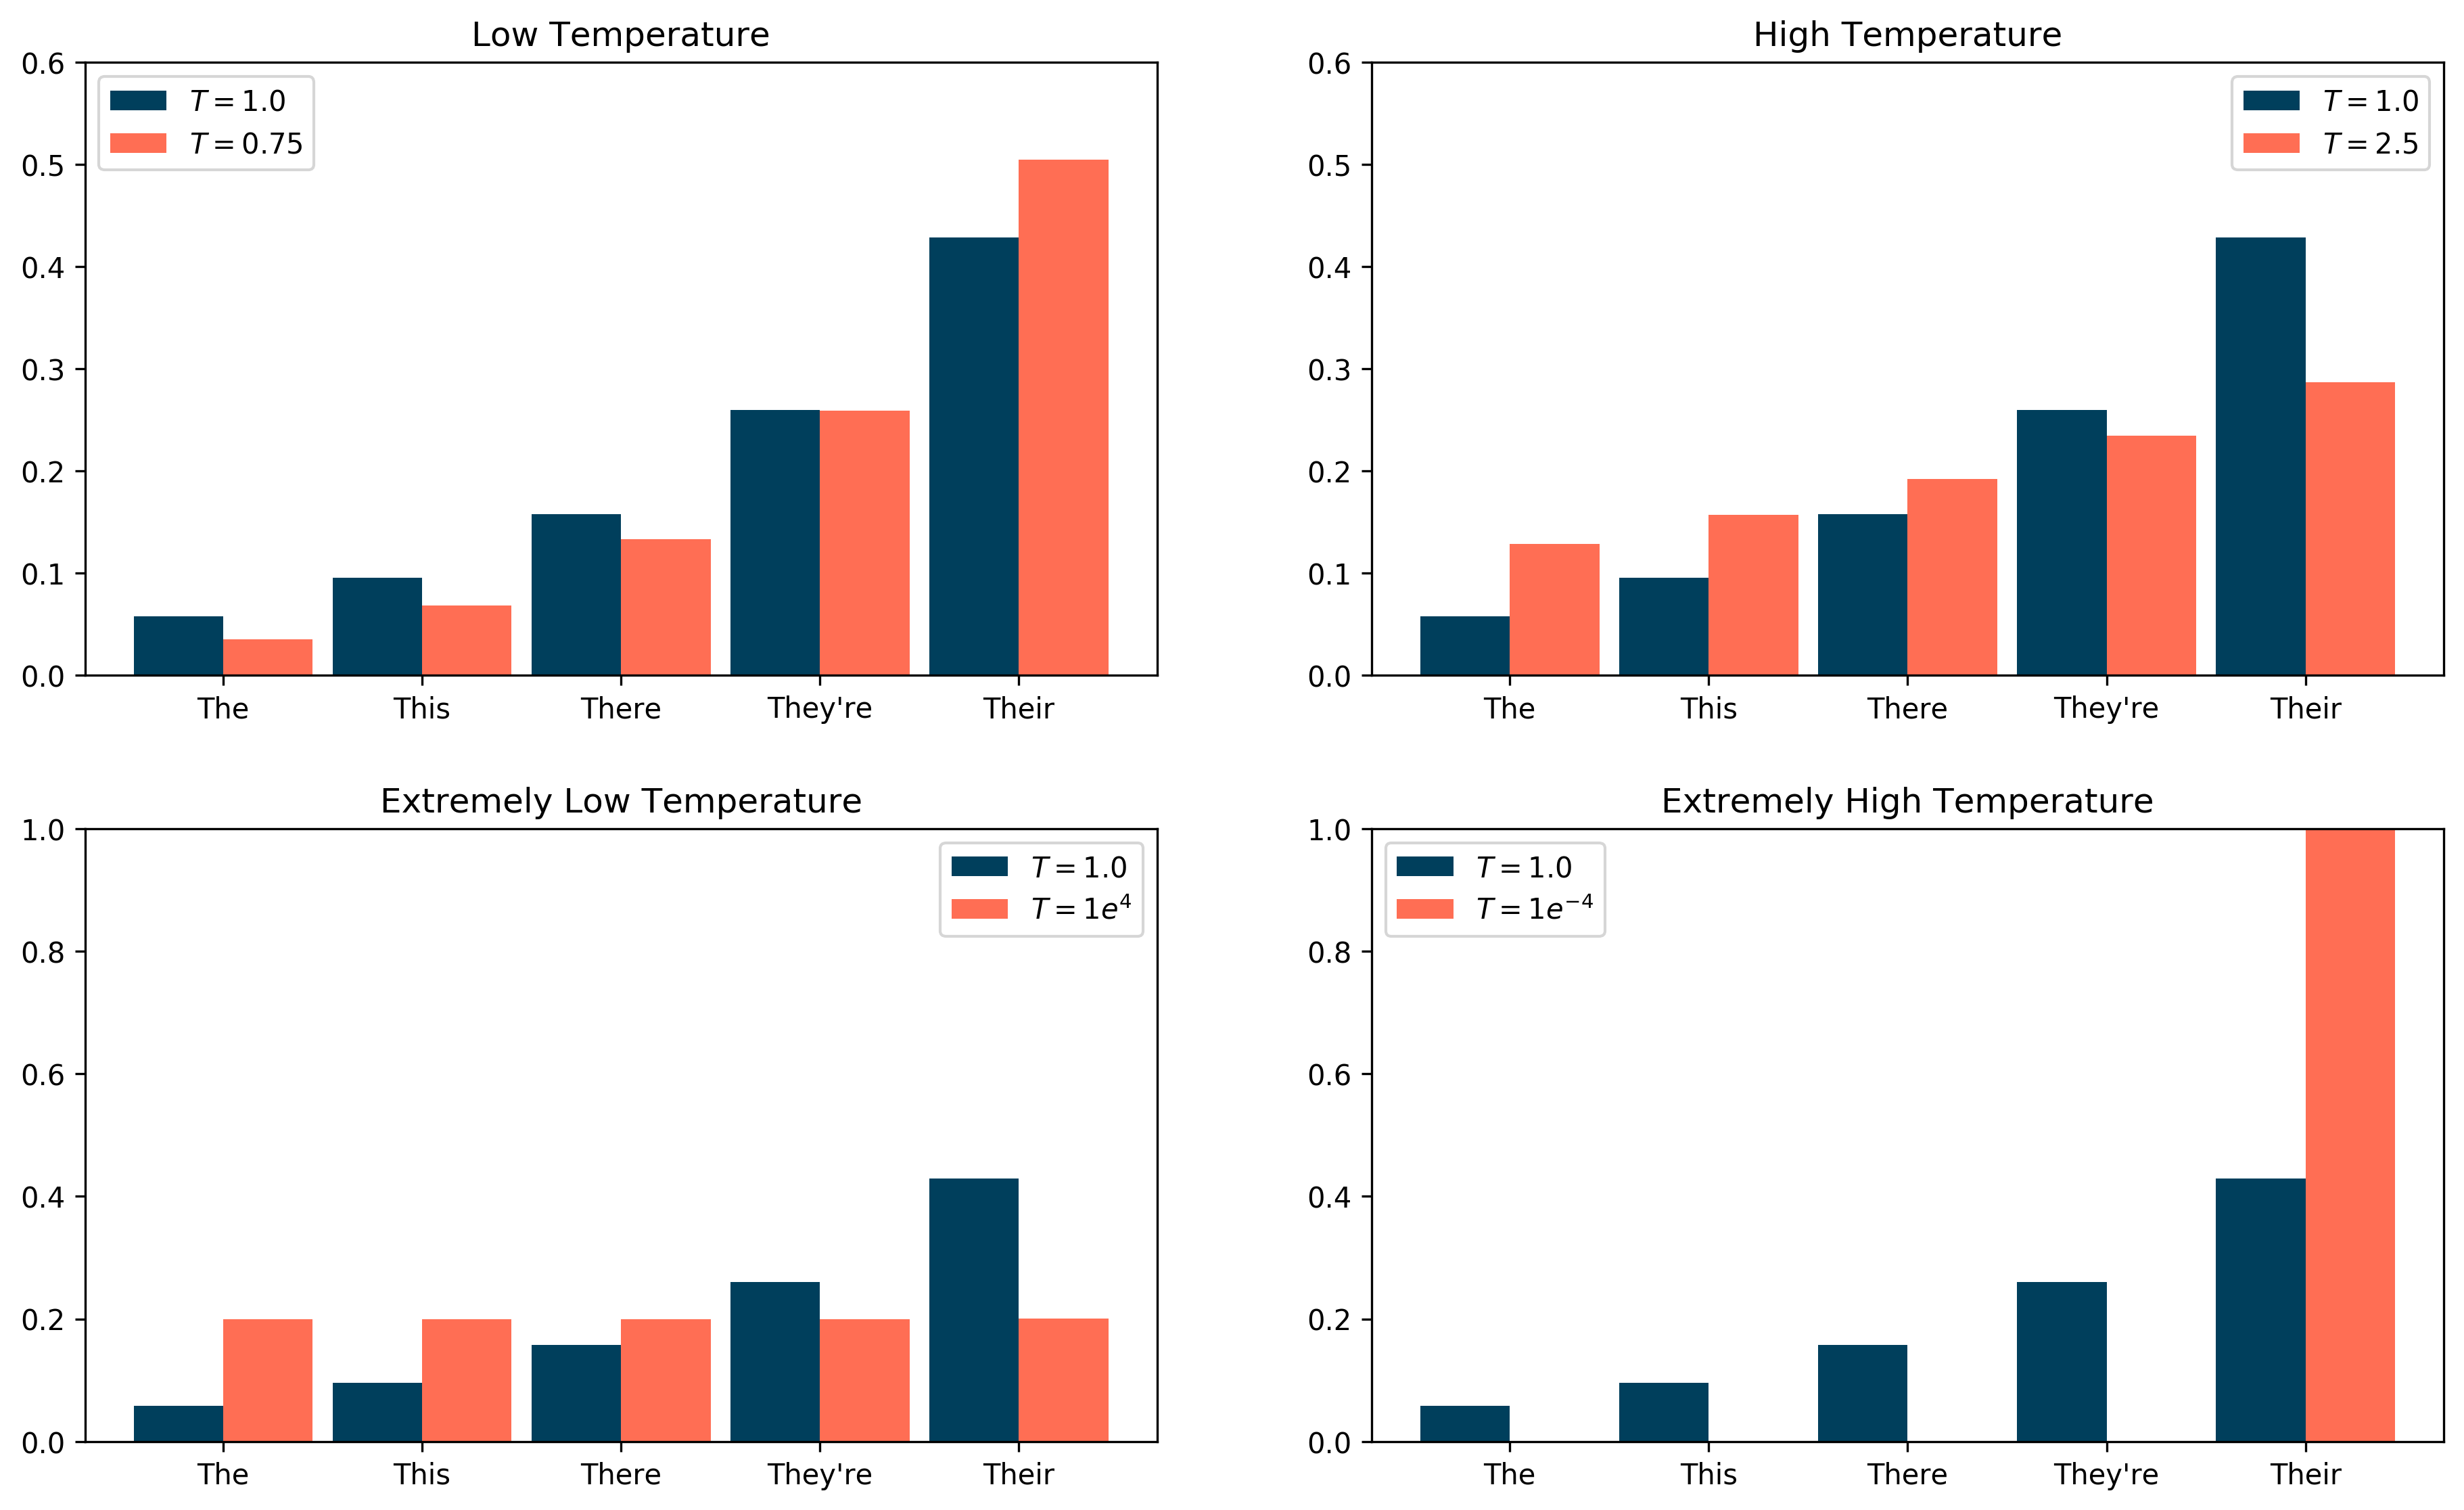
\includegraphics[width=10cm]{assets/temperature}
\end{figure}
\end{frame}

% \begin{frame}
%   \frametitle{Probability Refresher: Relationships between Discrete Distributions}
%   \begin{center}
%     \begin{tabular}{lcc}
%       \toprule
%       Distribution &  Categories &  Trials \\
%       \midrule
%       Bernoulli & 1 & 1 \\
%       Binomial & 1 & $n$ \\
%       Categorical & $k$ & 1 \\
%       Multinomial & $k$ & $n$ \\
%       \bottomrule
%     \end{tabular}
%   \end{center}
% \end{frame}

\begin{frame}
  \frametitle{Monte Carlo Decoding}
  \begin{itemize}
    \item Recall how we select the next token:
    \begin{itemize}
      \item \textbf{Greedy:} Top token weight
      \item \textbf{Teacher Forcing:} Randomly select the true token
    \end{itemize}
    \item Note that the outputs are a distribution over the target vocabulary
    \item \textbf{Use these weights in a multinomial to randomly select a continuation}
  \end{itemize}
  \begin{equation*}
      y_{i+1} \sim \text{Multinomial}\left( \theta_i \right)
  \end{equation*}
\end{frame}



\begin{frame}
  \frametitle{Different Token Decoding Schemes}
  \begin{itemize}
    \item \textbf{Greedy:}
  \end{itemize}
  \begin{equation*}
    y_{i+1} = \argmax_j \theta_i
  \end{equation*}
  \begin{itemize}
    \item \textbf{Teacher Forcing:}
  \end{itemize}
  \begin{equation*}
    y_{i+1} = \begin{cases}
      \argmax_{j} \theta_i  & \mathcal{U}(0, 1) < \text{TF} \\
      t_{i+1} & else
    \end{cases}
  \end{equation*}
  \begin{itemize}
    \item \textbf{Monte Carlo:}
  \end{itemize}
  \begin{equation*}
    y_{i+1} \sim \text{Multinomial}\left( \theta_i \right)
  \end{equation*}
  \begin{itemize}
    \item $\theta_i$ are the output weights from the Decoder
    \item $t_{i+1}$ is the true token at position $i + 1$
    \item $\text{TF}$ is the teacher forcing ratio
  \end{itemize}
\end{frame}

\begin{frame}
\frametitle{Masked Loss}
\begin{itemize}
  \item Remember, we don't care what gets predicted after seeing a $\textcolor{BrickRed}{\langle \texttt{EOS} \rangle}$
  \item Hence, we need to mask out the loss for predicted tokens associated with $\textcolor{WildStrawberry}{\langle \texttt{PAD} \rangle}$
\end{itemize}
\begin{equation*}
  \begin{array} {rccccccc}
    \texttt{pred} & \rightarrow & \textcolor{ForestGreen}{le} & \textcolor{ForestGreen}{le} & \textcolor{ForestGreen}{chat} & \textcolor{ForestGreen}{chat} & \textcolor{ForestGreen}{chat} & \textcolor{ForestGreen}{chat} \\
    {} & {} & \downarrow & \downarrow & \downarrow & \downarrow & \downarrow & \downarrow \\
    {} & {} & \ell & \ell & \ell & \ell & \ell & 0 \\
    {} & {} & \uparrow & \uparrow & \uparrow & \uparrow & \uparrow & \uparrow \\
    \texttt{true} & \rightarrow & \textcolor{ForestGreen}{le} & \textcolor{ForestGreen}{chat} & \textcolor{ForestGreen}{est} & \textcolor{ForestGreen}{noir} & \textcolor{BrickRed}{\langle \texttt{EOS} \rangle} & \textcolor{WildStrawberry}{\langle \texttt{PAD} \rangle} \\
  \end{array}
\end{equation*}
\begin{itemize}
  \item \textbf{Solution:} Zero out elements by either:
  \begin{itemize}
    \item Multiply pad outputs by $0$
    \item Specify the label to ignore in Cross Entropy call
  \end{itemize}
\end{itemize}
\begin{equation*}
  \ell(\mathbf{x}, y_i) = \mathds{1}_{\left\{y_i \not= \textcolor{WildStrawberry}{\langle \texttt{PAD} \rangle} \right\} } \cdot \left( -x_{y_i} + \log \sum_j \exp x_j \right)
\end{equation*}
\end{frame}

%%%%%%%%%%%%%%%%%%%%%%%%%%%%%%%%%%%%%%%%%%%%%%%%%%%%%%%%%%%%%%%%%%%%%%%%%%%%%%%%
\section{Initial Training Results}

\begin{frame}
  \frametitle{Recall: Seq2Seq Architecture}
  \begin{figure}
    \centering
    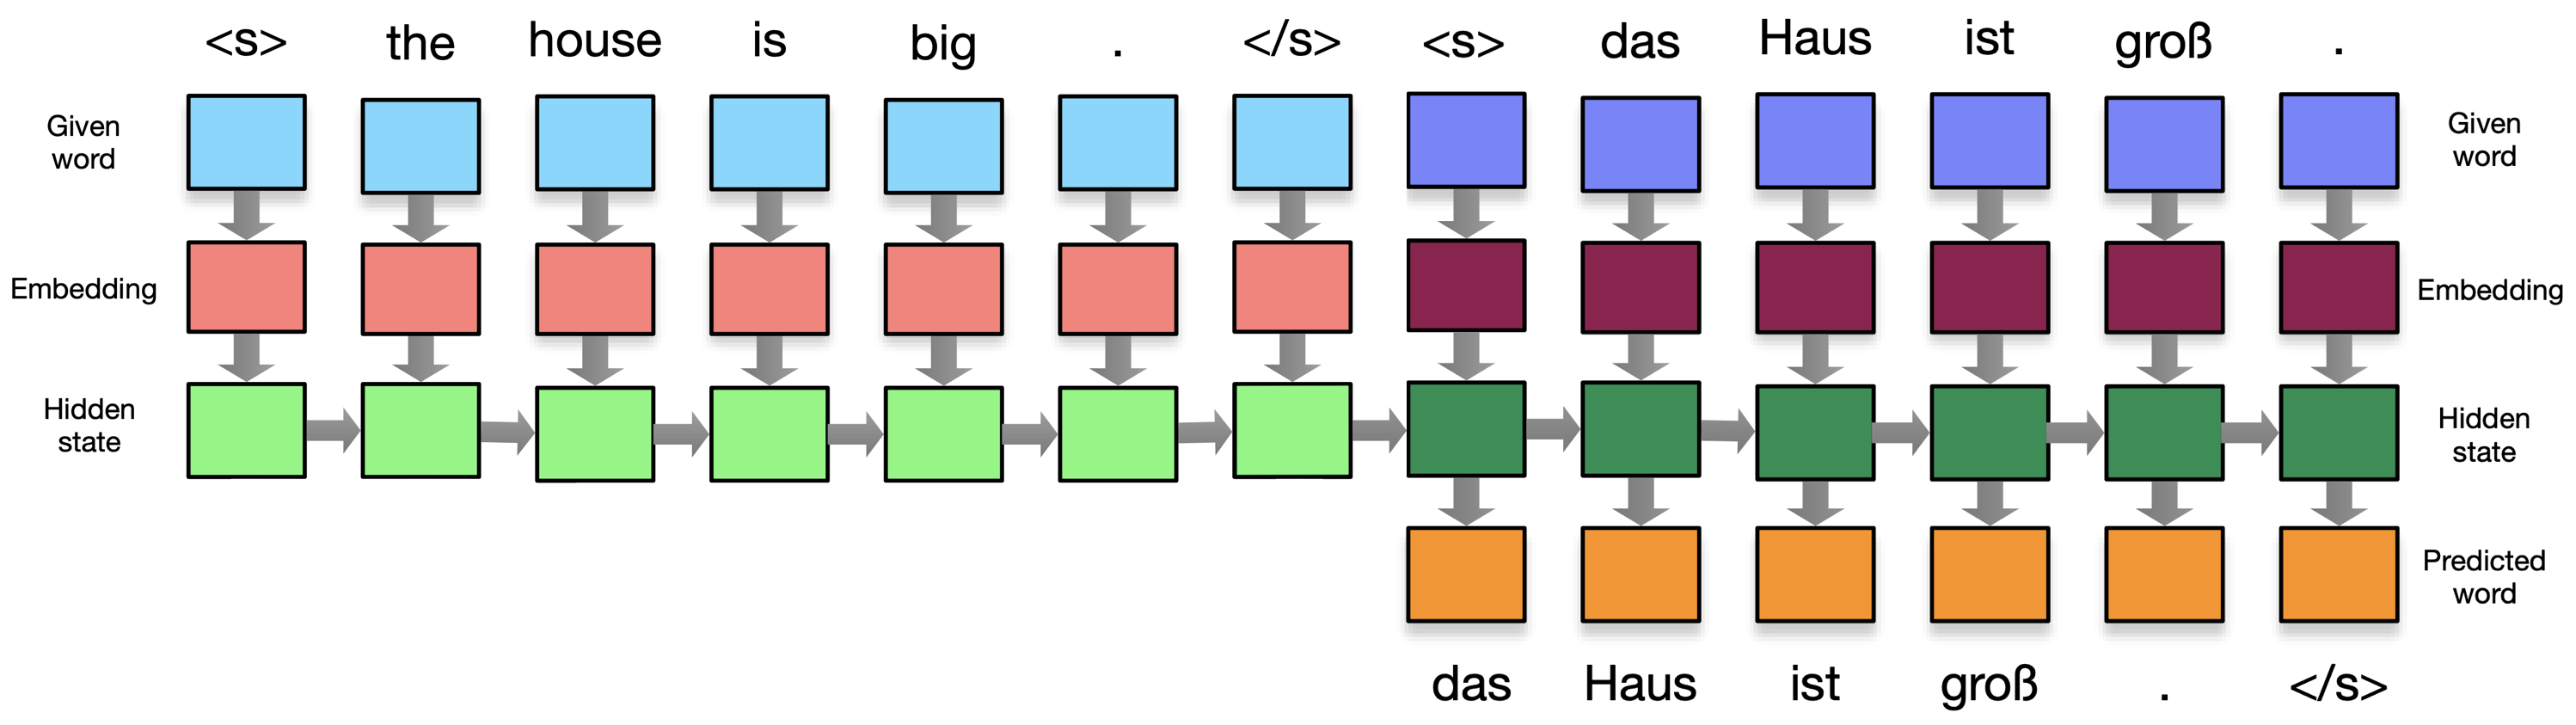
\includegraphics[width=10cm, valign=c]{assets/enc-dec}
  \end{figure}
  % add picture from notebook
  \begin{figure}
    \centering
    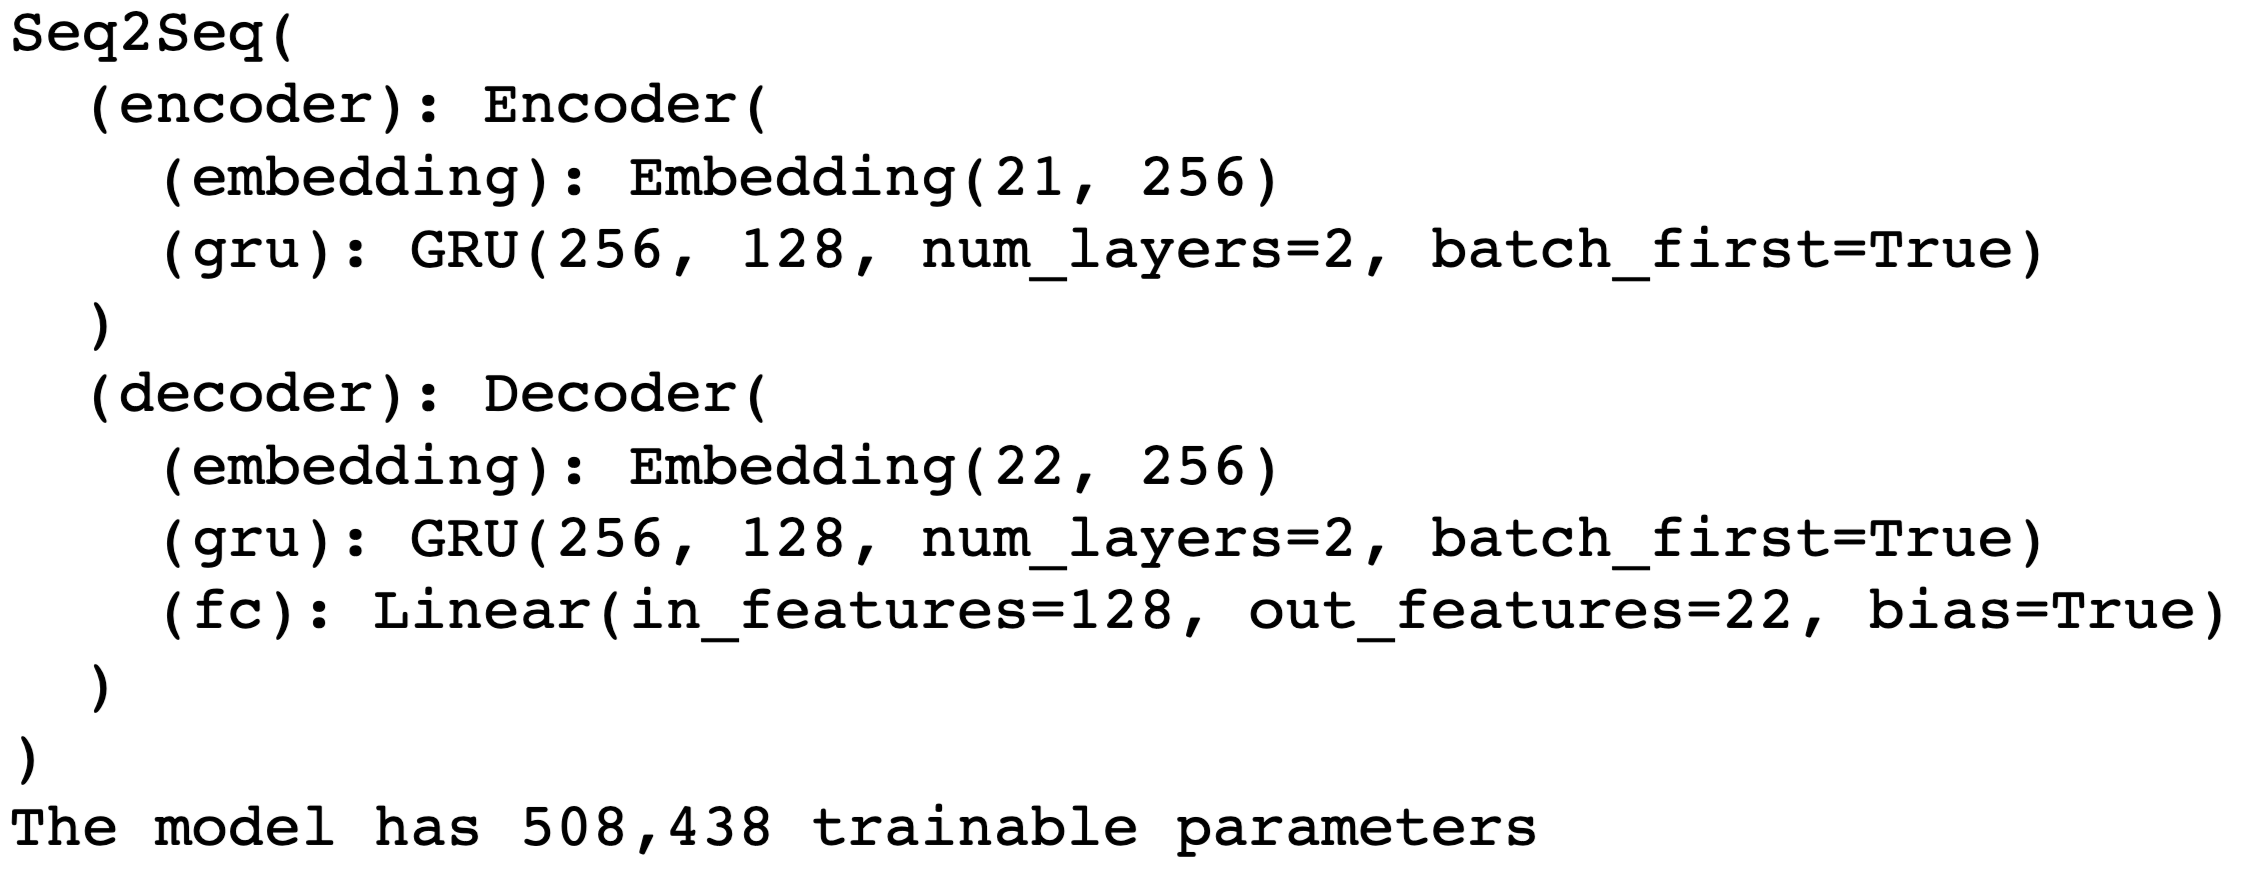
\includegraphics[width=10cm, valign=c]{assets/col-seq2seq}
  \end{figure}
\end{frame}

\begin{frame}
  \frametitle{Seq2Seq: Sample Results}
  \begin{equation*}
    \textcolor{ForestGreen}{
    \begin{array}{cl}
      \texttt{>} & \texttt{num num num punct} \\
      \texttt{=} & \texttt{num \textcolor{WildStrawberry}{$\langle$SEG$\rangle$} num \textcolor{WildStrawberry}{$\langle$SEG$\rangle$} num \textcolor{WildStrawberry}{$\langle$SEG$\rangle$} punct} \\
      \texttt{<} & \texttt{num \textcolor{WildStrawberry}{$\langle$SEG$\rangle$} num \textcolor{WildStrawberry}{$\langle$SEG$\rangle$} num \textcolor{WildStrawberry}{$\langle$SEG$\rangle$} punct} \\
      \\
      \texttt{>} & \texttt{adj num num num} \\
      \texttt{=} & \texttt{adj \textcolor{WildStrawberry}{$\langle$SEG$\rangle$} num \textcolor{WildStrawberry}{$\langle$SEG$\rangle$} num \textcolor{WildStrawberry}{$\langle$SEG$\rangle$} num} \\
      \texttt{<} & \texttt{adj \textcolor{WildStrawberry}{$\langle$SEG$\rangle$} num \textcolor{WildStrawberry}{$\langle$SEG$\rangle$} num \textcolor{WildStrawberry}{$\langle$SEG$\rangle$} num num num num num} \\
      \\
      \texttt{>} & \texttt{verb noun noun noun noun noun verb} \\
      \texttt{=} & \texttt{verb \textcolor{WildStrawberry}{$\langle$SEG$\rangle$} noun noun \textcolor{WildStrawberry}{$\langle$SEG$\rangle$} noun noun noun \textcolor{WildStrawberry}{$\langle$SEG$\rangle$} verb} \\
      \texttt{<} & \texttt{verb noun \textcolor{WildStrawberry}{$\langle$SEG$\rangle$} \textcolor{WildStrawberry}{$\langle$SEG$\rangle$} noun noun noun noun \textcolor{WildStrawberry}{$\langle$SEG$\rangle$} noun } \cdots \\
    \end{array}}
  \end{equation*}
\end{frame}

\begin{frame}
  \frametitle{Translation Results: TL;DR}
  \begin{itemize}
    \item Reasonably for small sequences
    \item Struggles to terminate properly
    \begin{itemize}
      \item Maybe more training?
    \end{itemize}
    \item Long Sequences are a mess
    \pause
    \item \textbf{However} this indicates that enough noise can be transfered via the hidden state
  \end{itemize}
\end{frame}

\begin{frame}
  \frametitle{Review}
  \begin{itemize}
    \item We have covered:
    \begin{itemize}
      \item What are Seq2Seq Models?
      \item How can I reduce my vocabulary size?
      \item How do I train a Seq2Seq model?
    \end{itemize}
    \item Part 2 will explore more advanced concepts such as:
    \begin{itemize}
      \item Decoding with Beam Search
      \item Modeling Recurrent Relations
      \item Other applications of Sequence Modeling
    \end{itemize}
  \end{itemize}
\end{frame}

%%%%%%%%%%%%%%%%%%%%%%%%%%%%%%%%%%%%%%%%%%%%%%%%%%%%%%%%%%%%%%%%%%%%%%%%%%%%%%%%

\section{Thank You!}

%%%%%%%%%%%%%%%%%%%%%%%%%%%%%%%%%%%%%%%%%%%%%%%%%%%%%%%%%%%%%%%%%%%%%%%%%%%%%%%%
%%%%%%%%%%%%%%%%%%%%%%%%%%%%%%%%%%%%%%%%%%%%%%%%%%%%%%%%%%%%%%%%%%%%%%%%%%%%%%%%
%%%%%%%%%%%%%%%%%%%%%%%%%%%%%%%%%%%%%%%%%%%%%%%%%%%%%%%%%%%%%%%%%%%%%%%%%%%%%%%%
\title{Seq2Seq in Action: Column Segmentation}
\subtitle{Part 2}
\date{January 23, 2020}

\begin{frame}
\titlepage
\end{frame}
% \section{Seq2Seq in Action: Advanced Techniques\\Part 2\\January 23, 2020}

\begin{frame}
  \frametitle{Review}
  \begin{itemize}
    \item We have covered:
    \begin{itemize}
      \item What are Seq2Seq Models?
      \item How can I reduce my vocabulary size?
      \item How do I train a Seq2Seq model?
    \end{itemize}
    \item Part 2 will explore more advanced concepts such as:
    \begin{itemize}
      \item Decoding with Beam Search
      \item Modeling Recurrent Relations
      \item Other applications of Sequence Modeling
    \end{itemize}
  \end{itemize}
\end{frame}

%%%%%%%%%%%%%%%%%%%%%%%%%%%%%%%%%%%%%%%%%%%%%%%%%%%%%%%%%%%%%%%%%%%%%%%%%%%%%%%%
\section{Decoding: Making better Translations}

\begin{frame}
  \frametitle{Beam Search}
  \begin{itemize}
    \item Beam Search is a technique to explore different translation paths
    \item Based on the idea that you \textbf{shouldn't take the greedy path}
    \item And that the best path may be sub-optimal during early iterations
  \end{itemize}
\end{frame}

\begin{frame}
\frametitle{Beam Search}
\begin{figure}
  \centering
  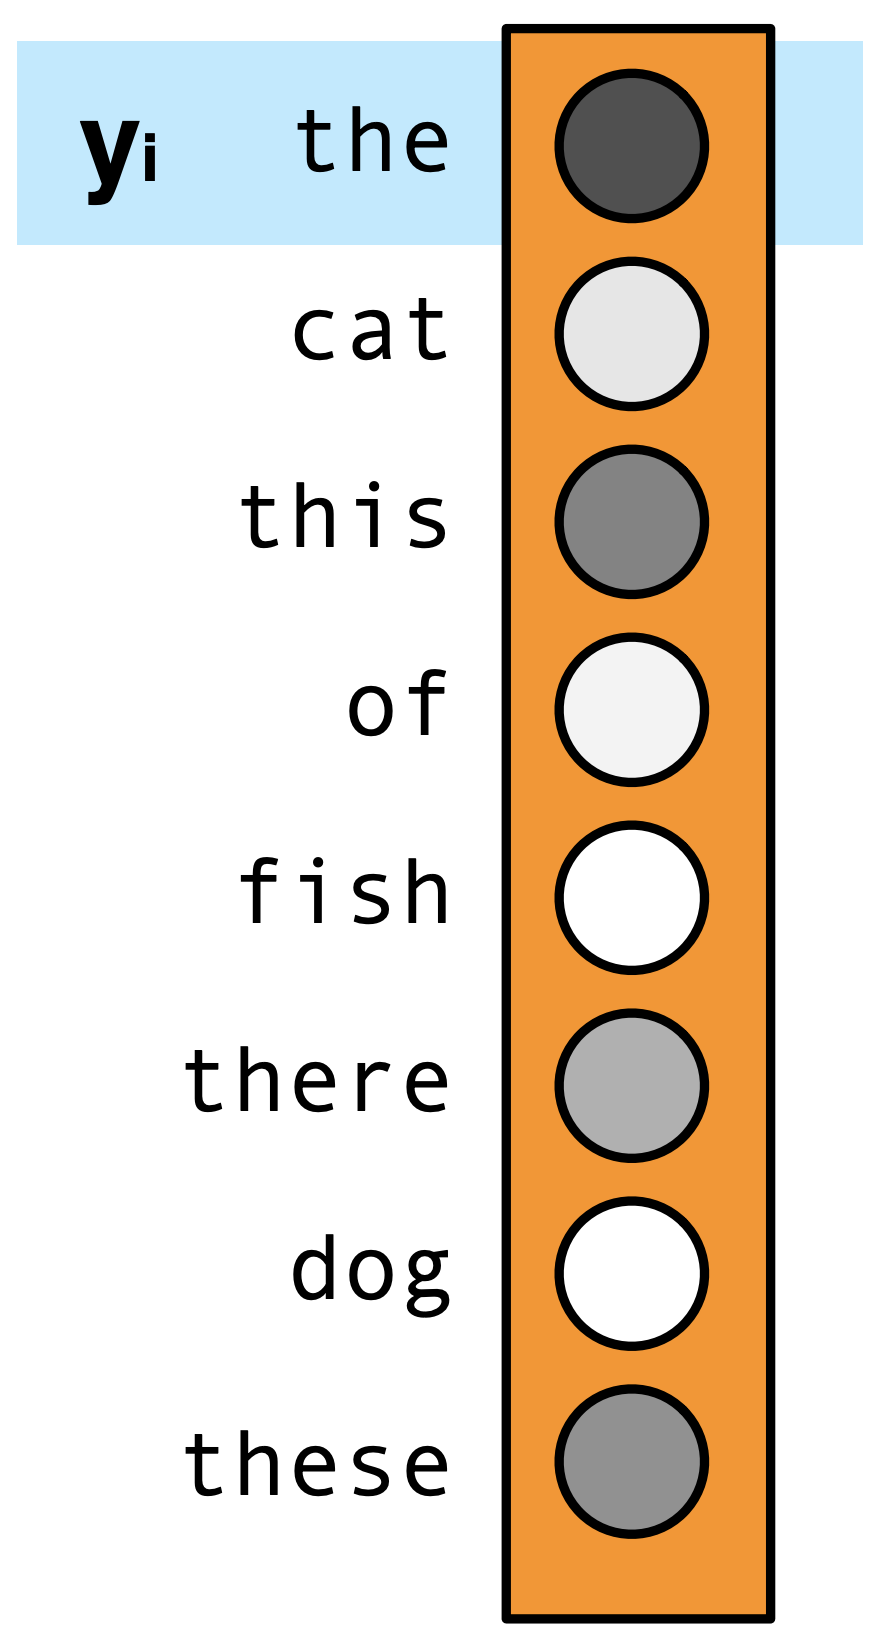
\includegraphics[height=5cm, valign=c]{assets/beam1}
\end{figure}
\end{frame}

\begin{frame}
\frametitle{Beam Search}
\begin{figure}
  \centering
  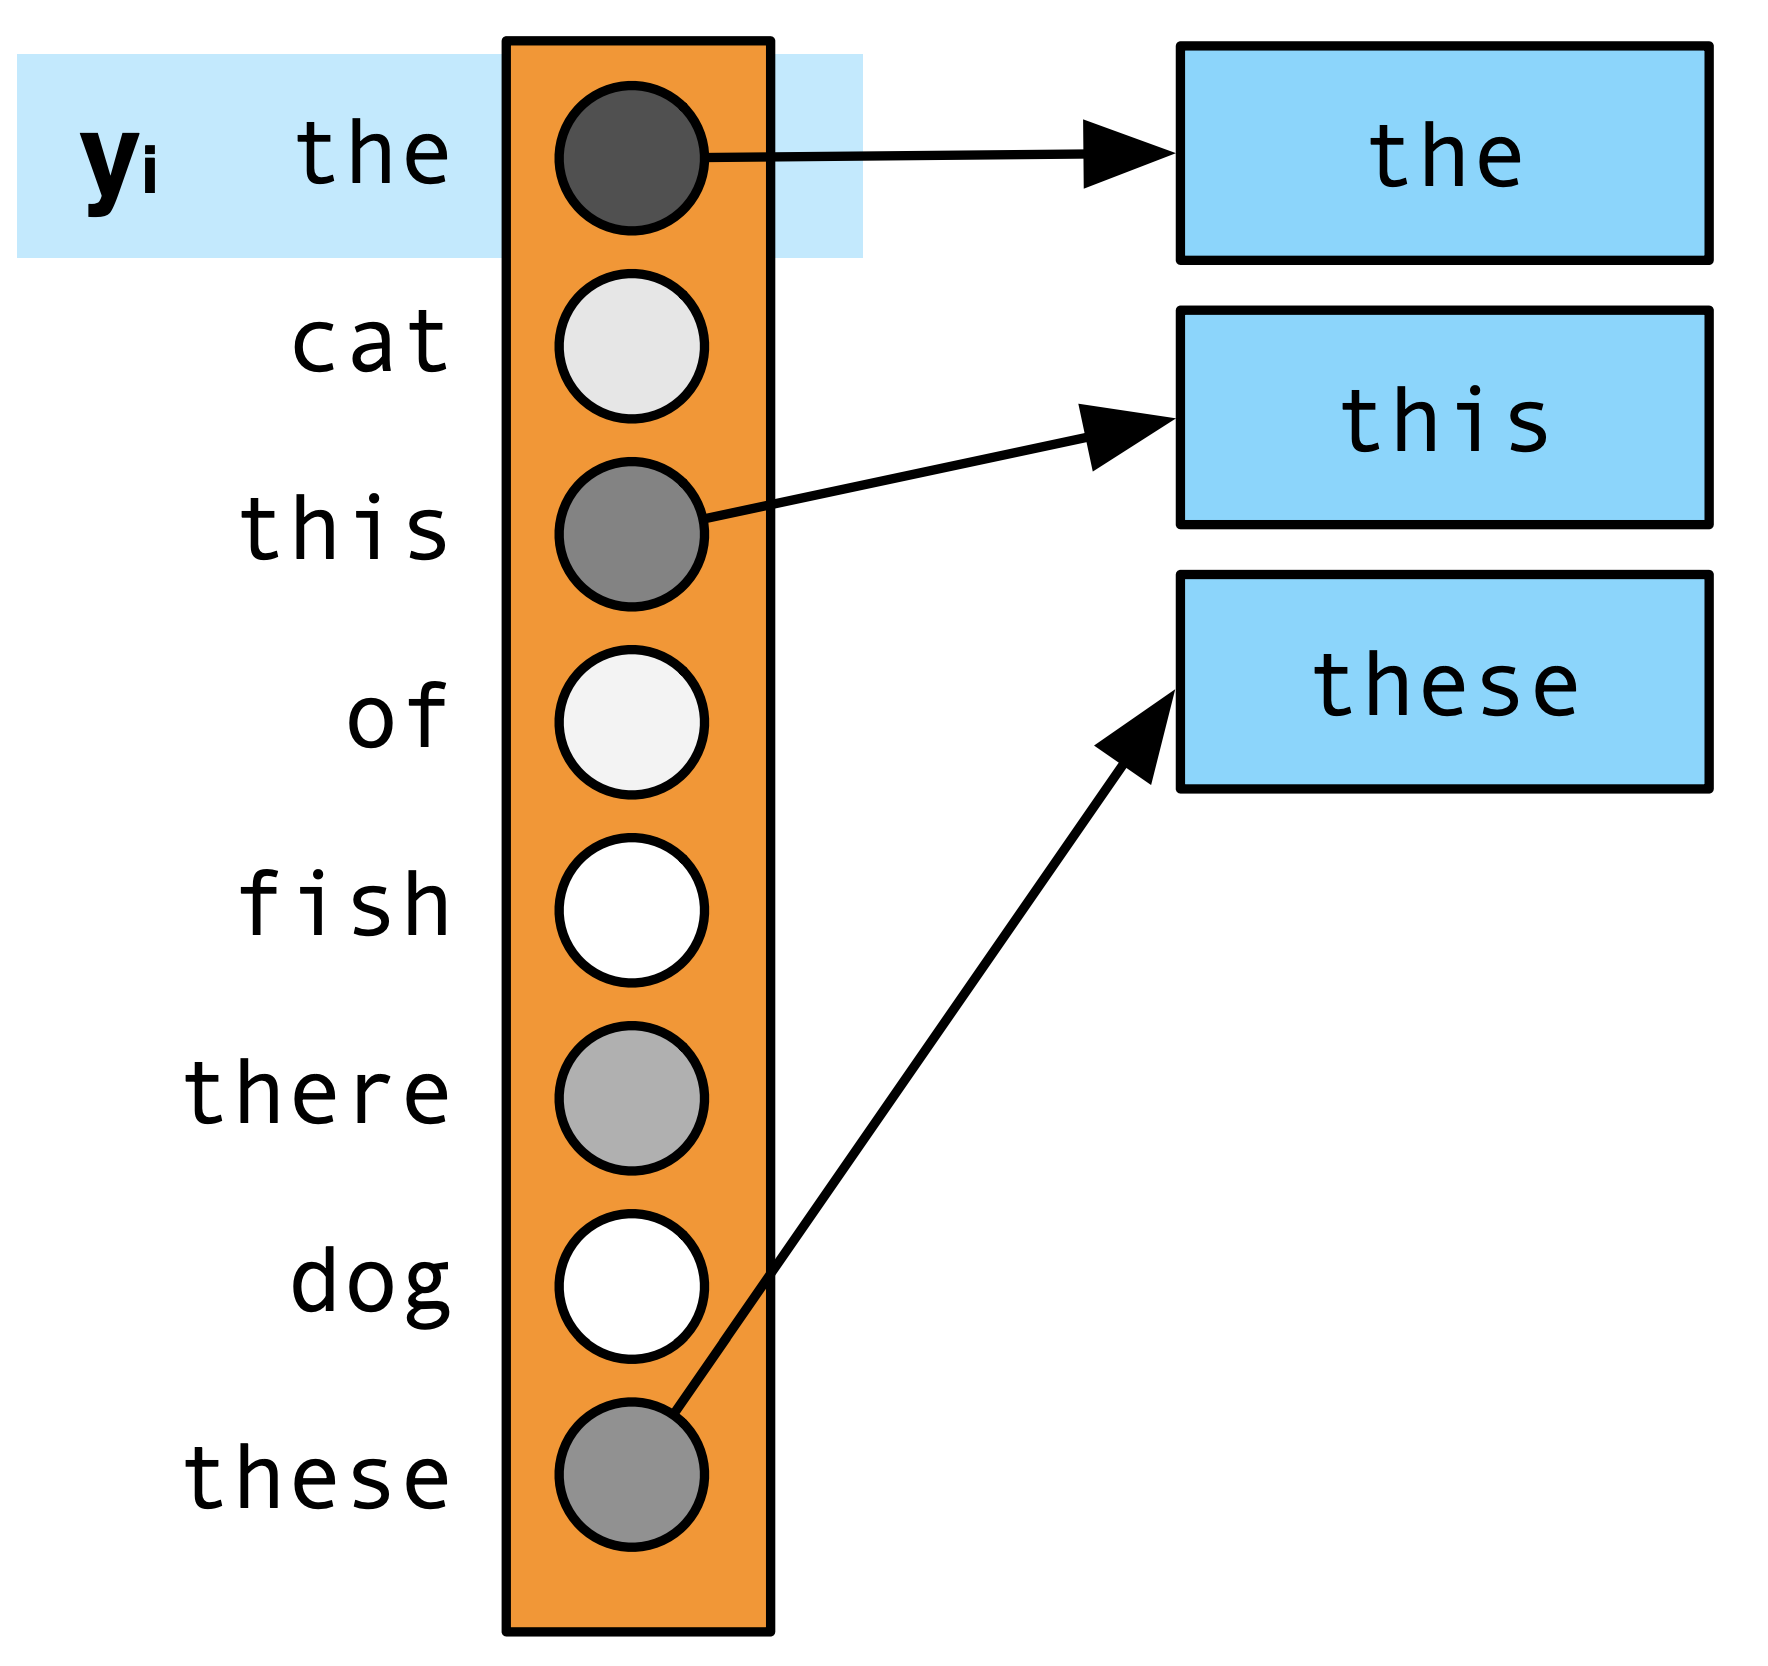
\includegraphics[height=5cm, valign=c]{assets/beam2}
\end{figure}
\end{frame}

\begin{frame}
\frametitle{Beam Search}
\begin{figure}
  \centering
  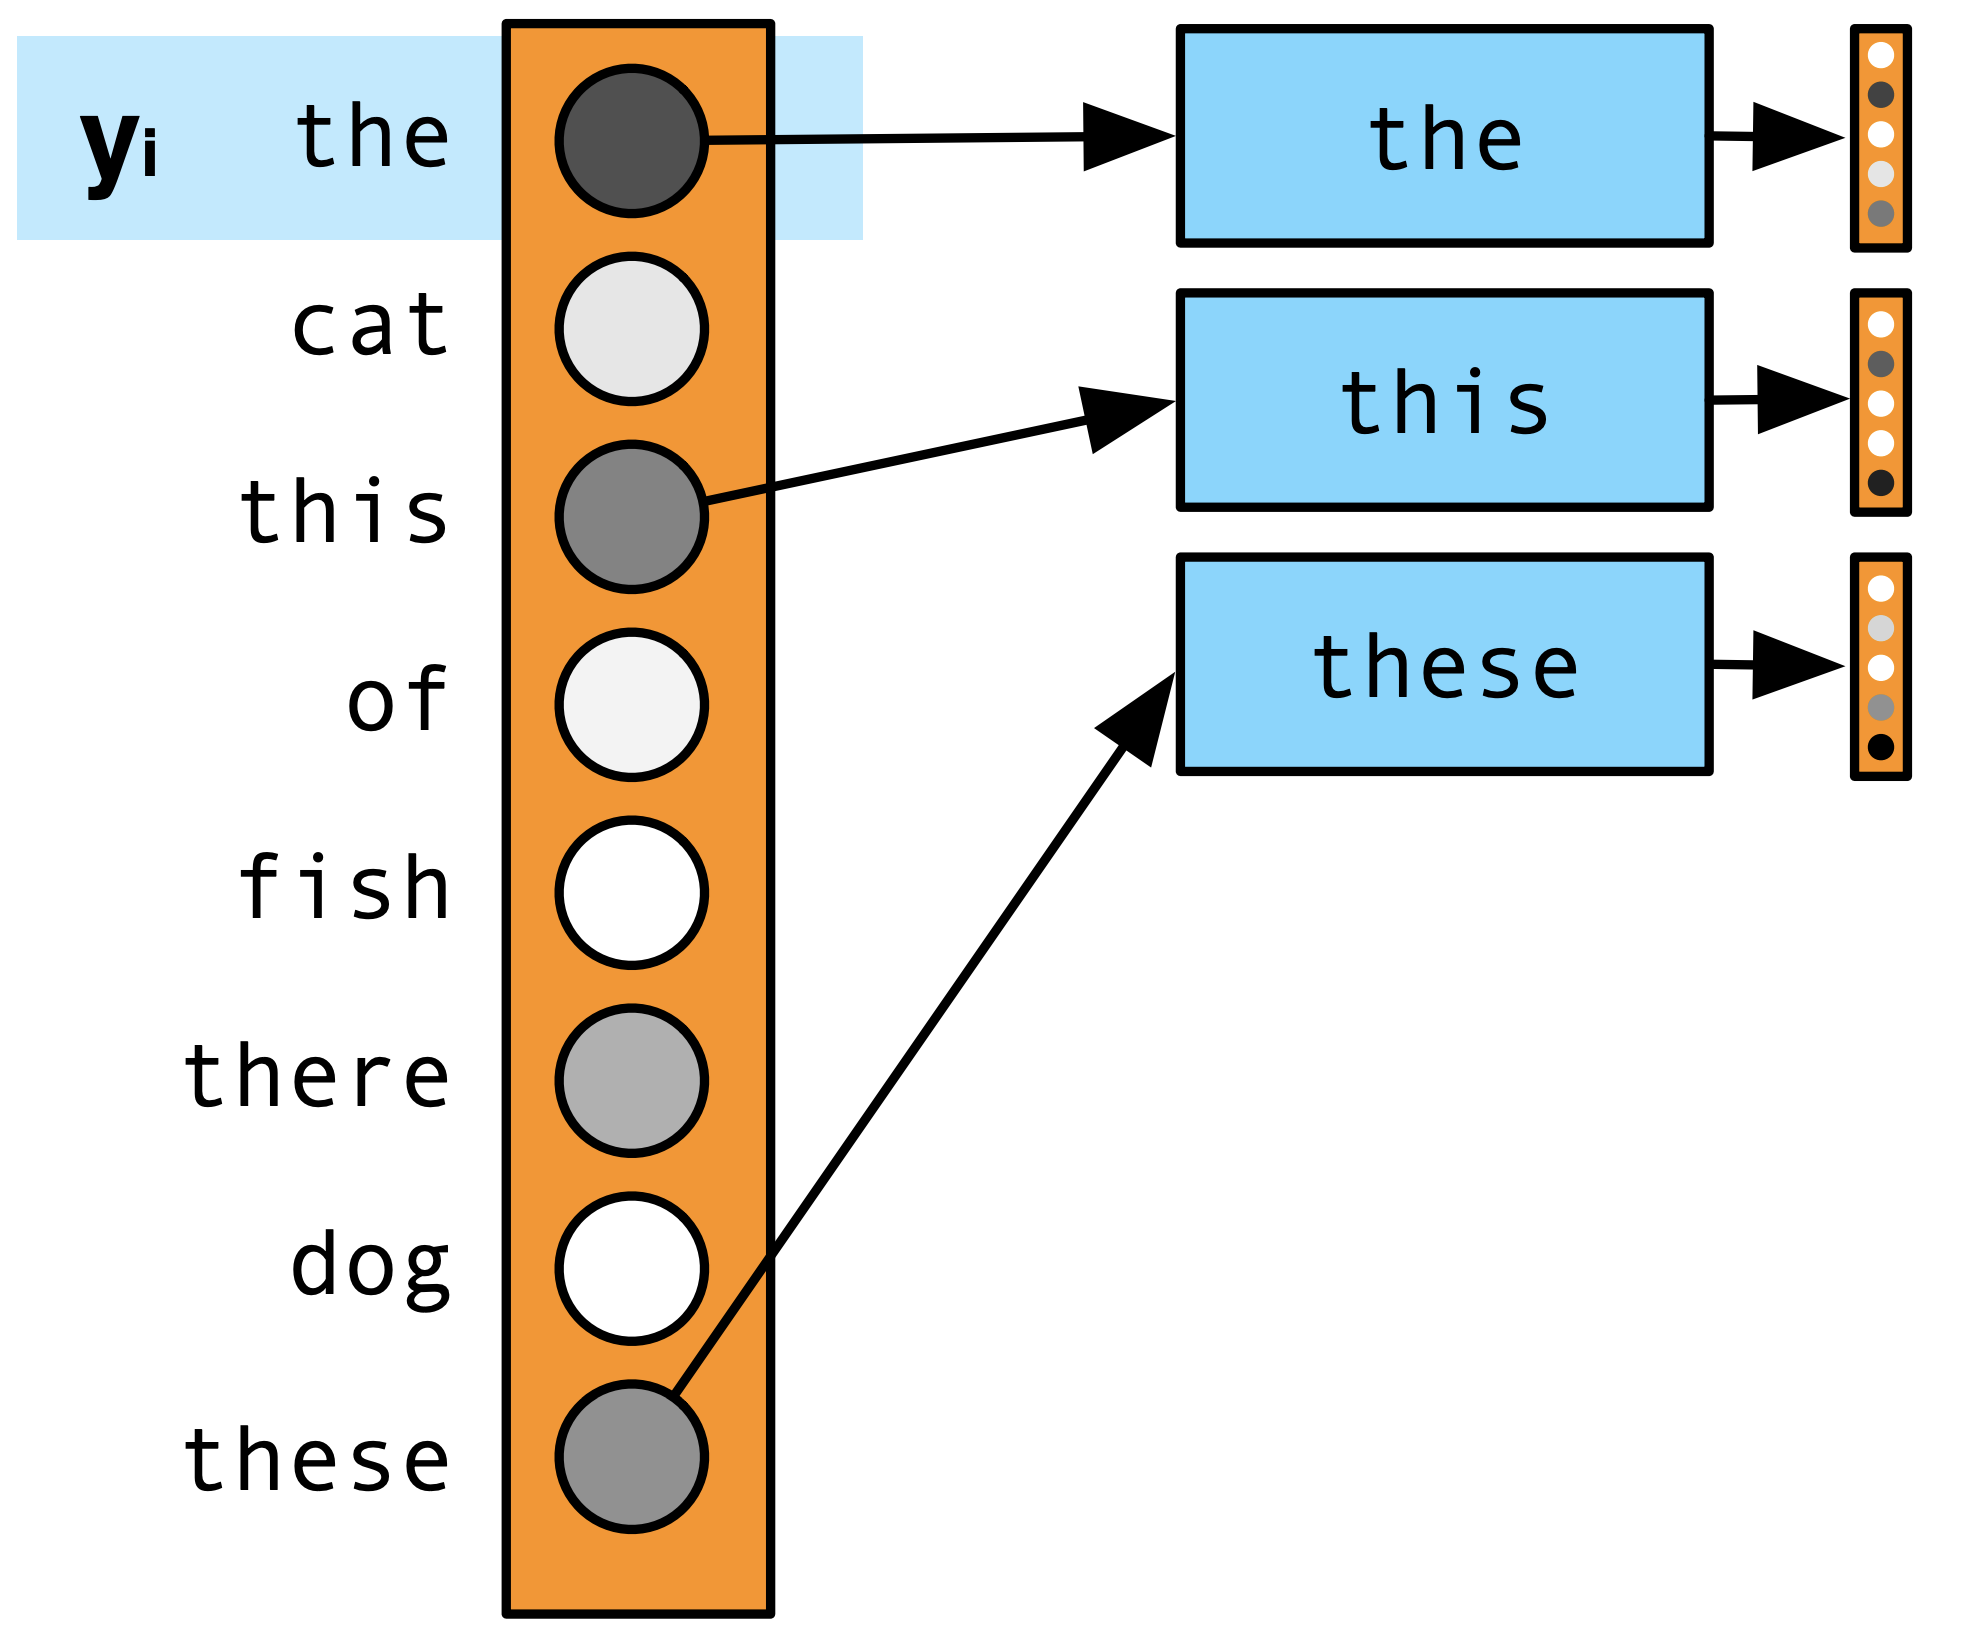
\includegraphics[height=5cm, valign=c]{assets/beam3}
\end{figure}
\end{frame}

\begin{frame}
\frametitle{Beam Search}
\begin{figure}
  \centering
  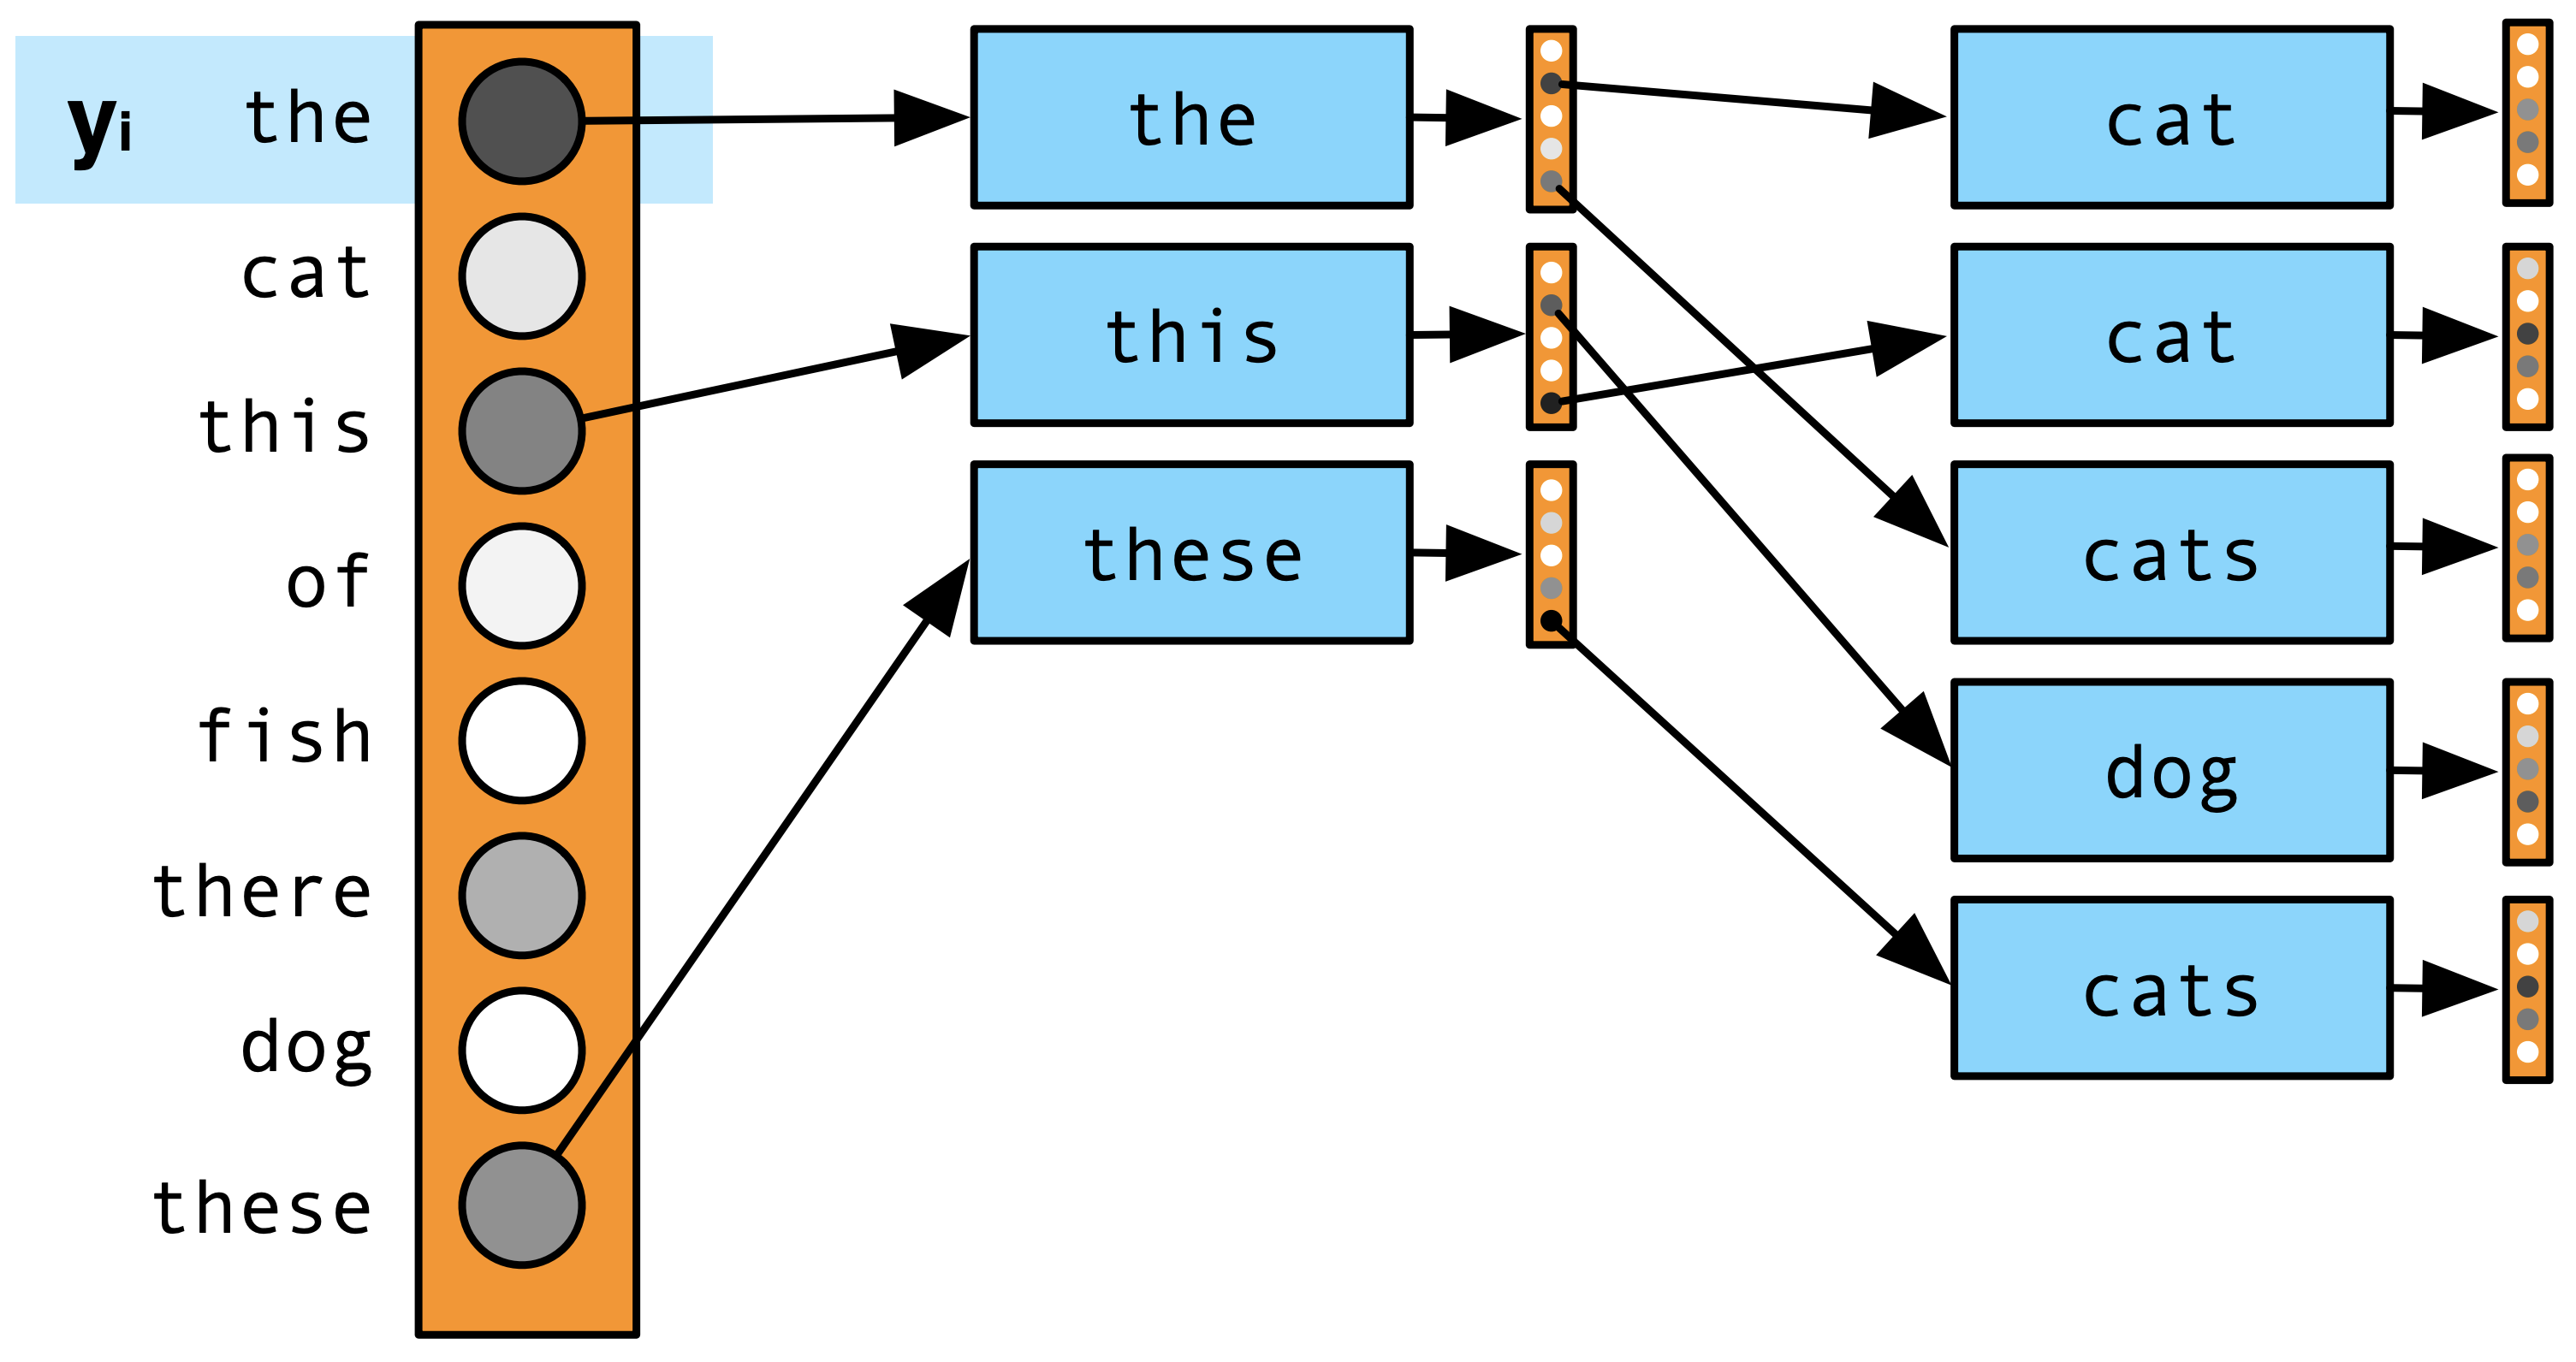
\includegraphics[height=5cm, valign=c]{assets/beam4}
\end{figure}
\end{frame}

\begin{frame}
\frametitle{Beam Search}
\begin{figure}
  \centering
  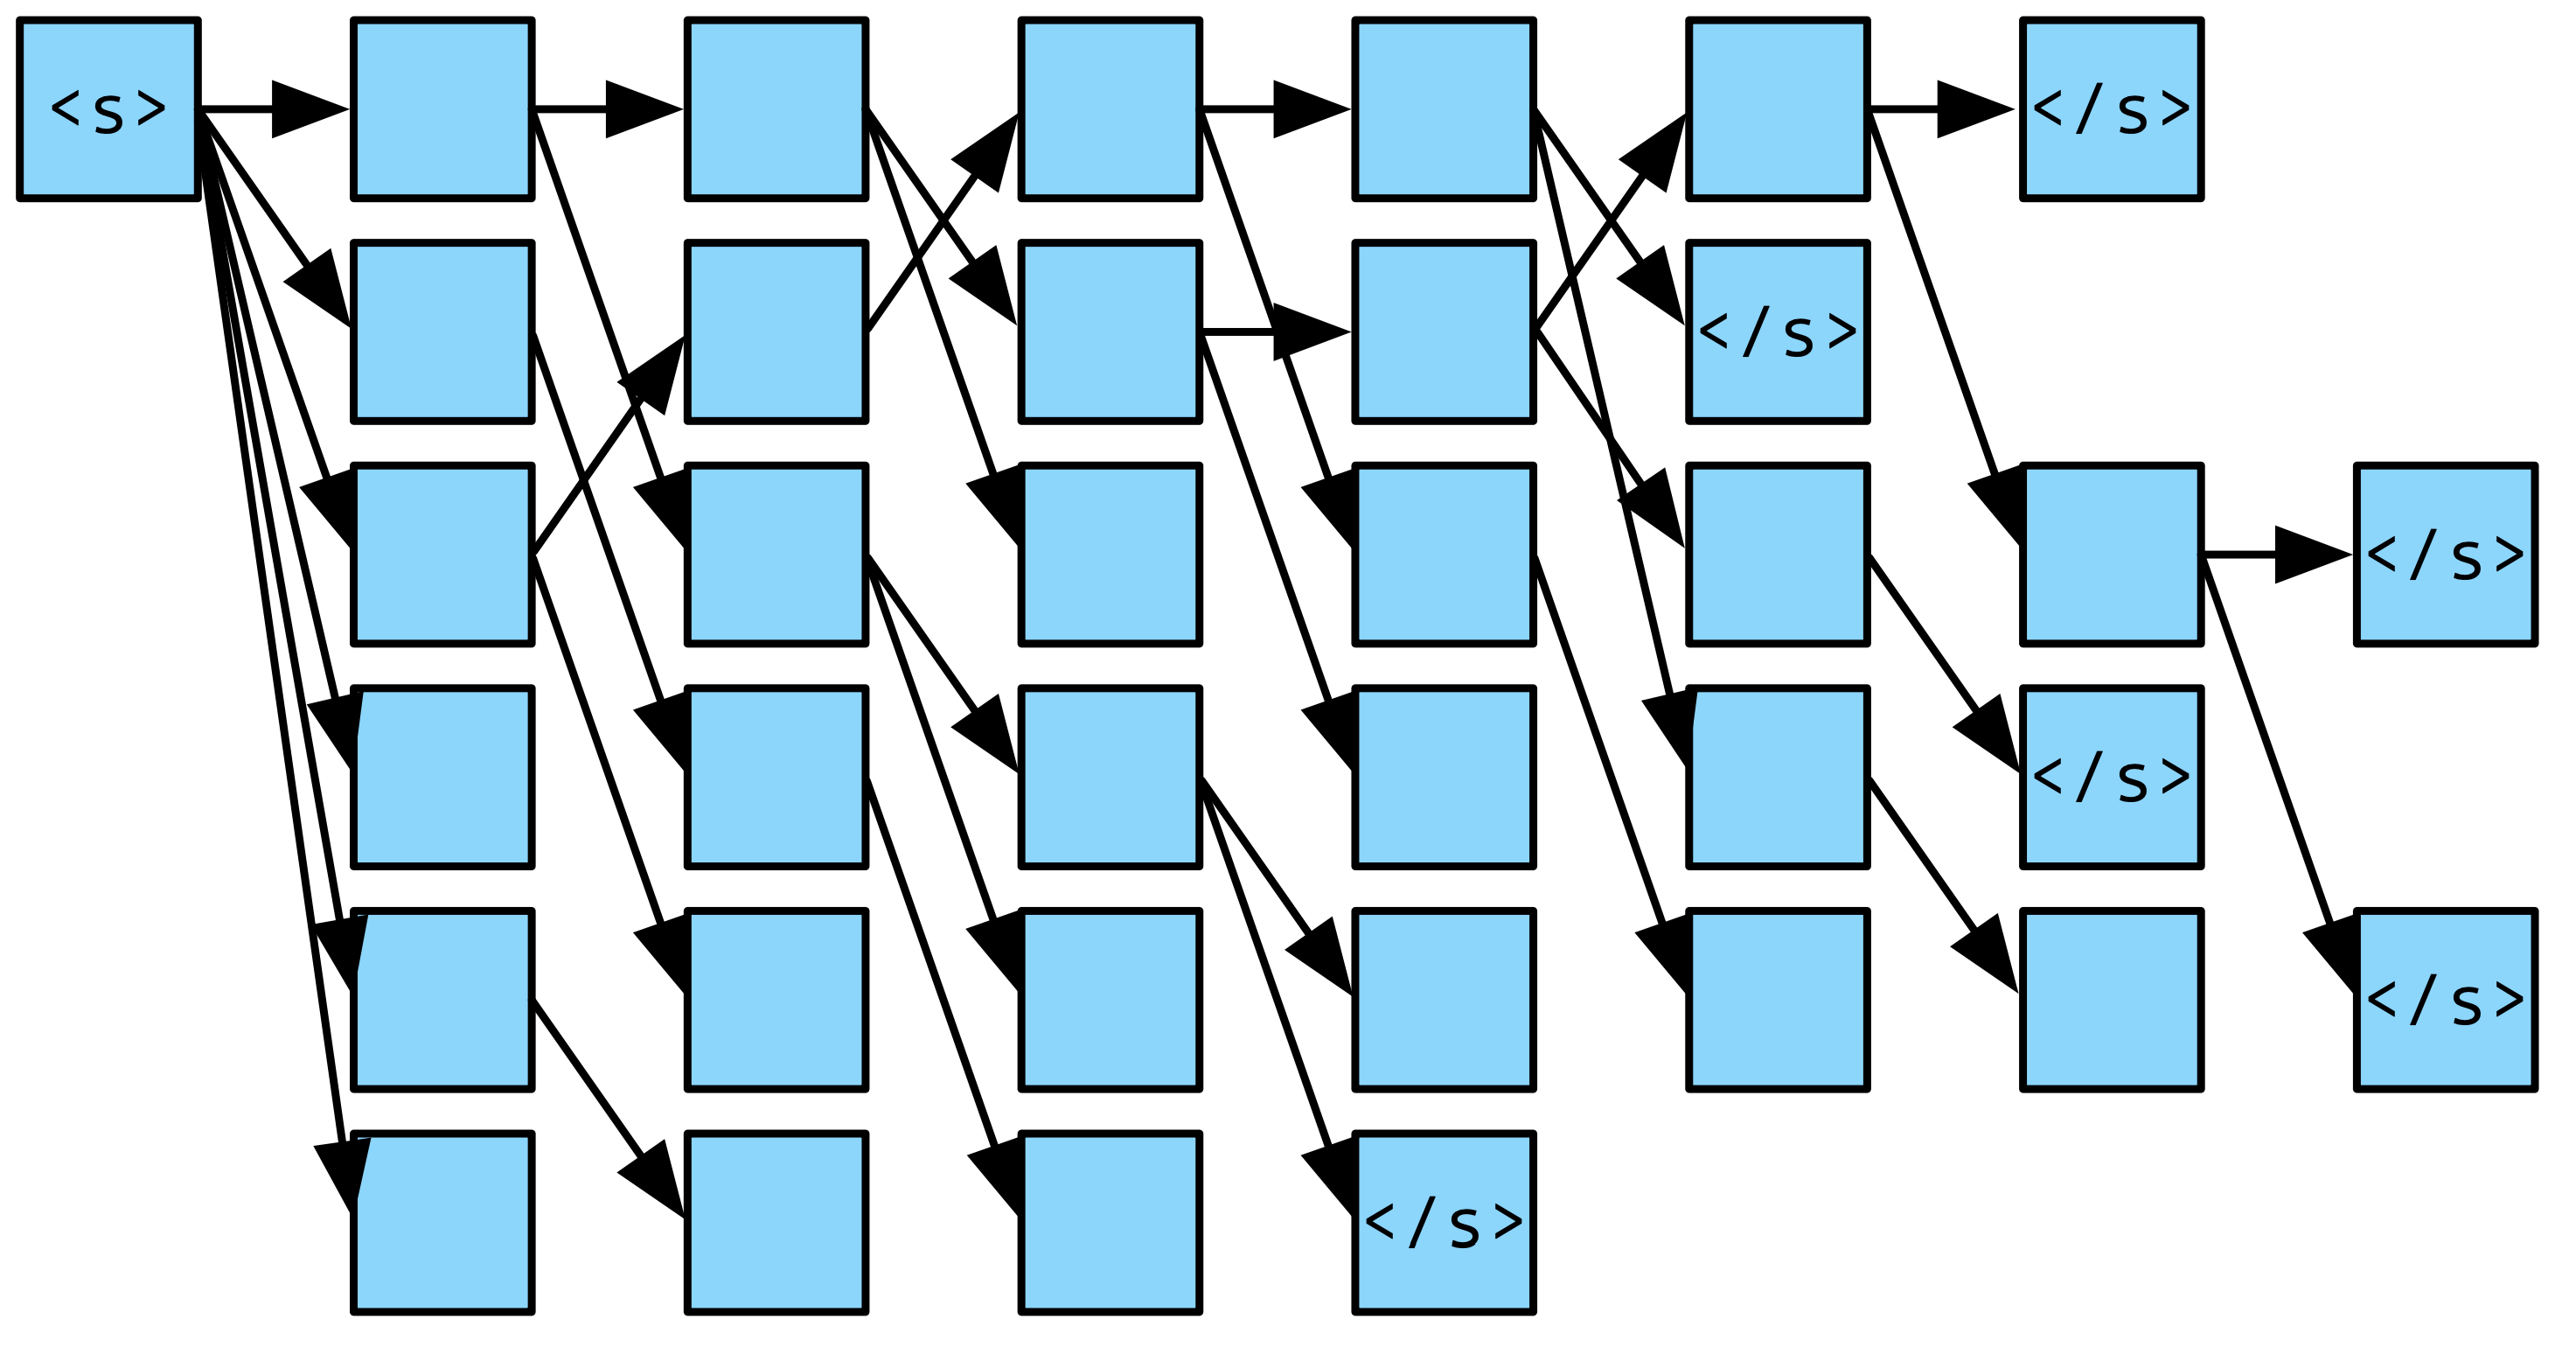
\includegraphics[height=5cm, valign=c]{assets/beam5}
\end{figure}
\end{frame}

\begin{frame}
\frametitle{Beam Search}
\begin{figure}
  \centering
  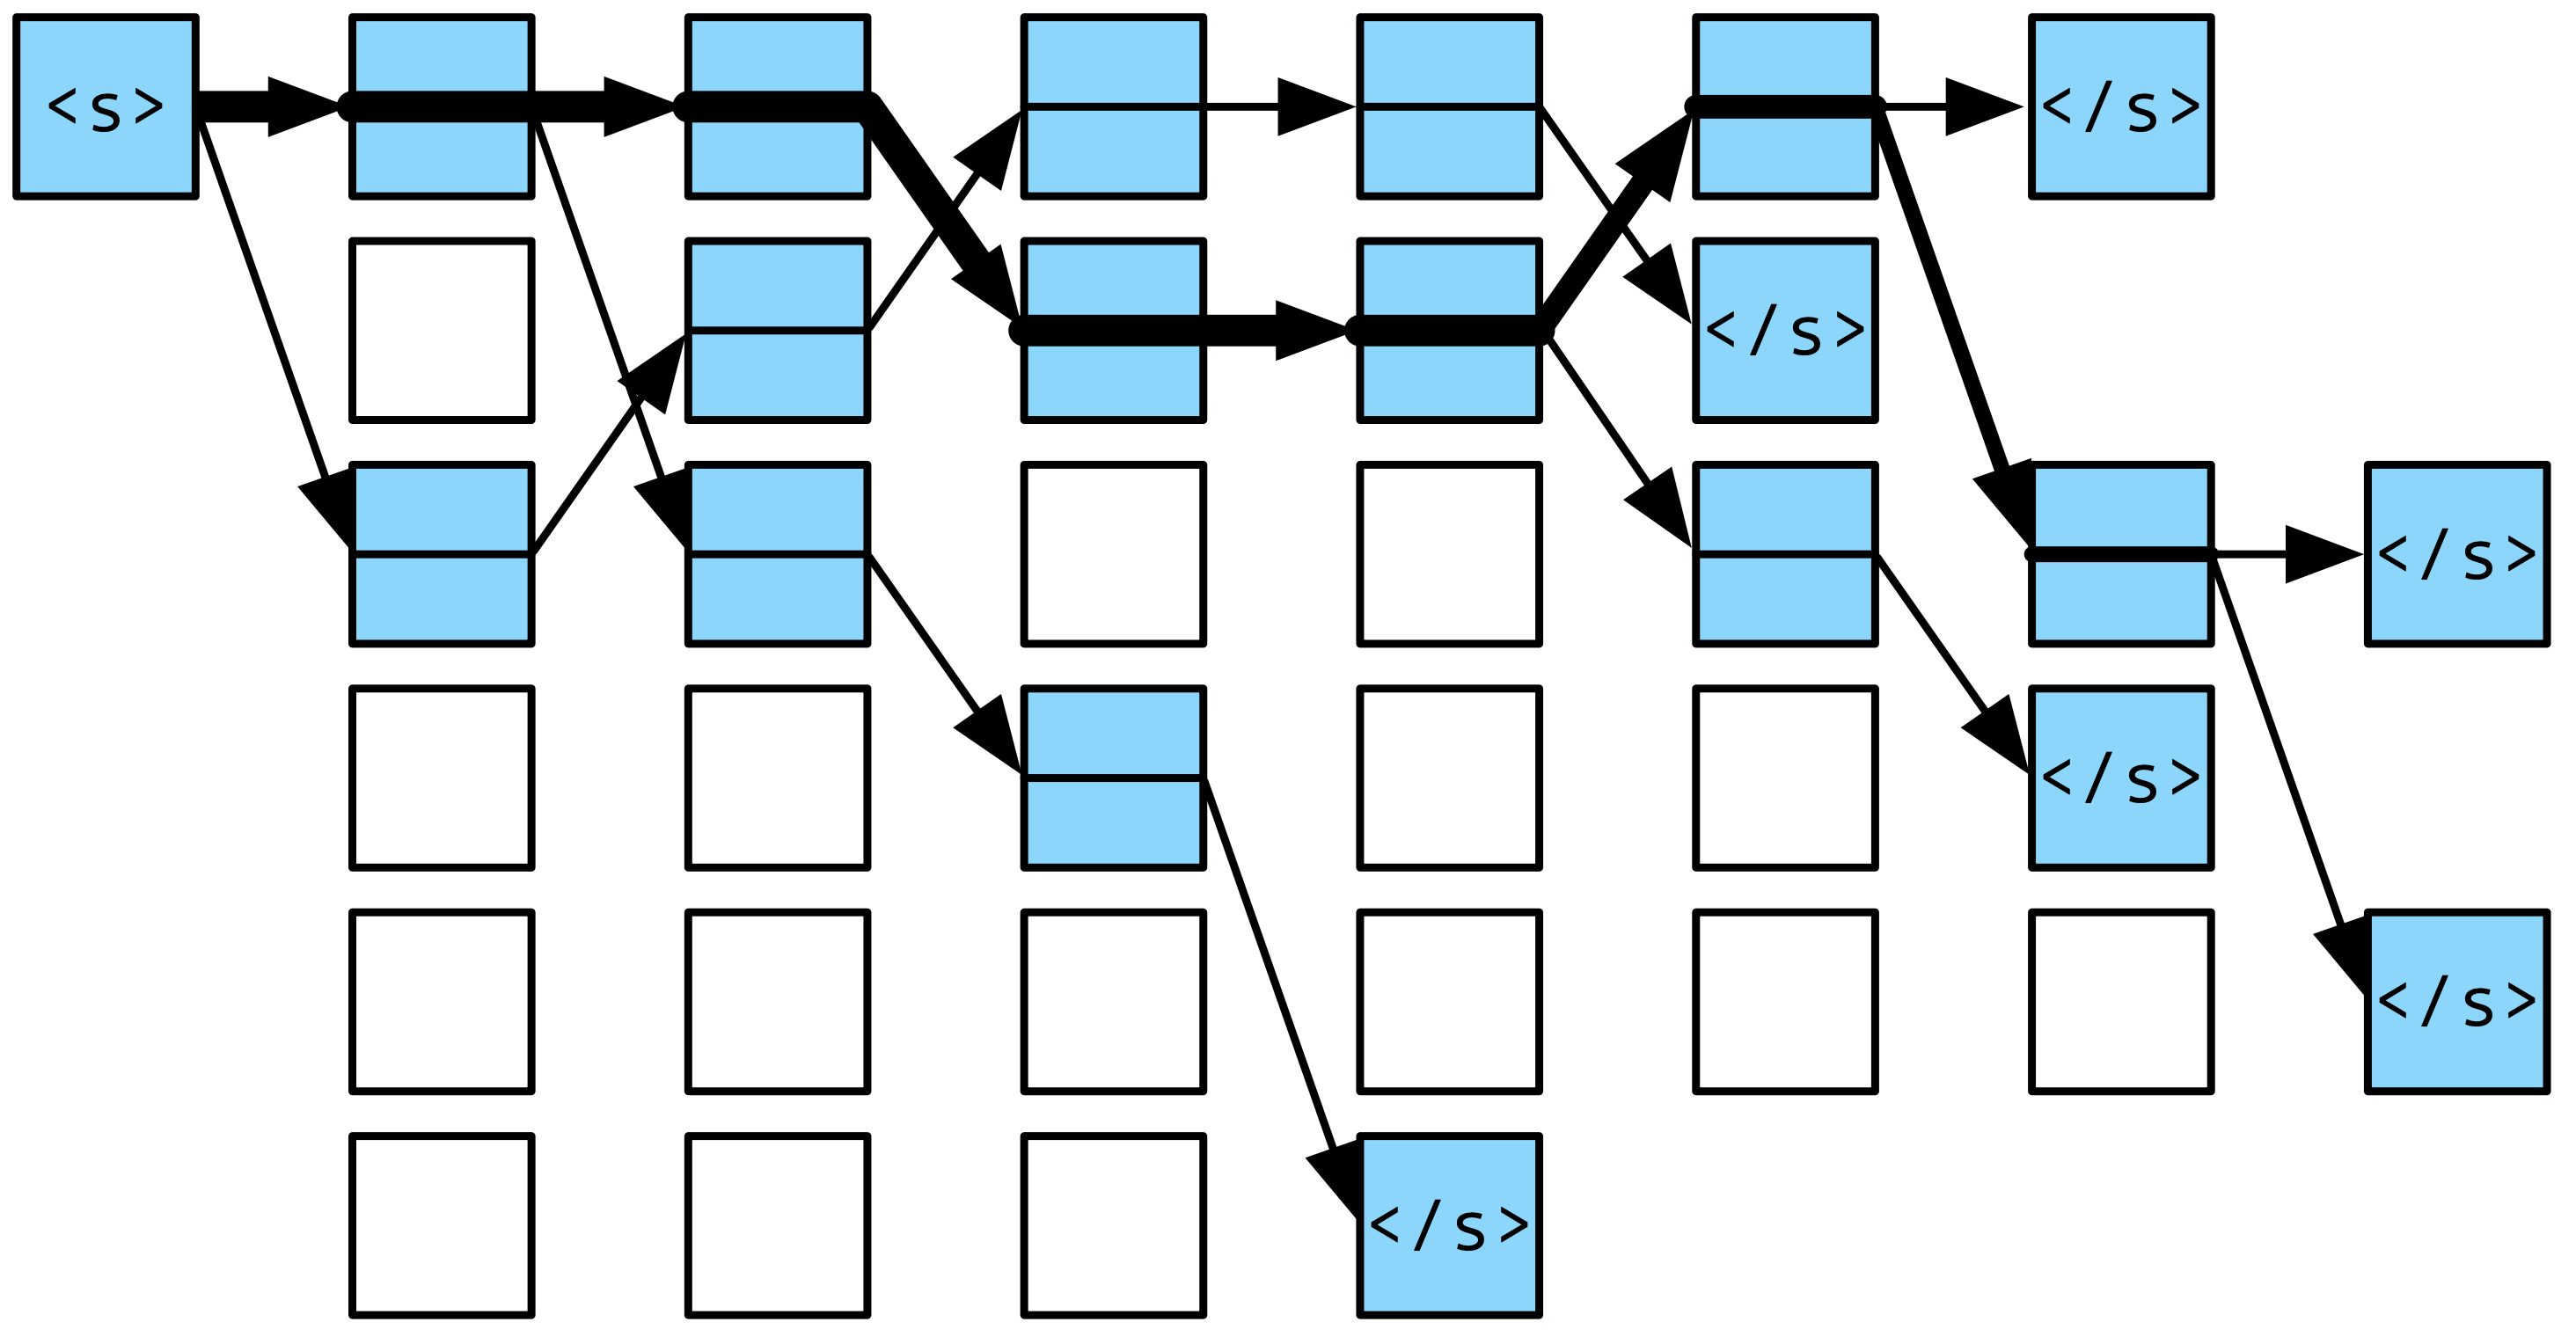
\includegraphics[height=5cm, valign=c]{assets/beam6}
\end{figure}
\end{frame}

\begin{frame}
\frametitle{Monte Carlo Beam Search}
  \begin{figure}
    \centering
    $y_{i+1} \; \sim \; \text{Multinomial} \left( 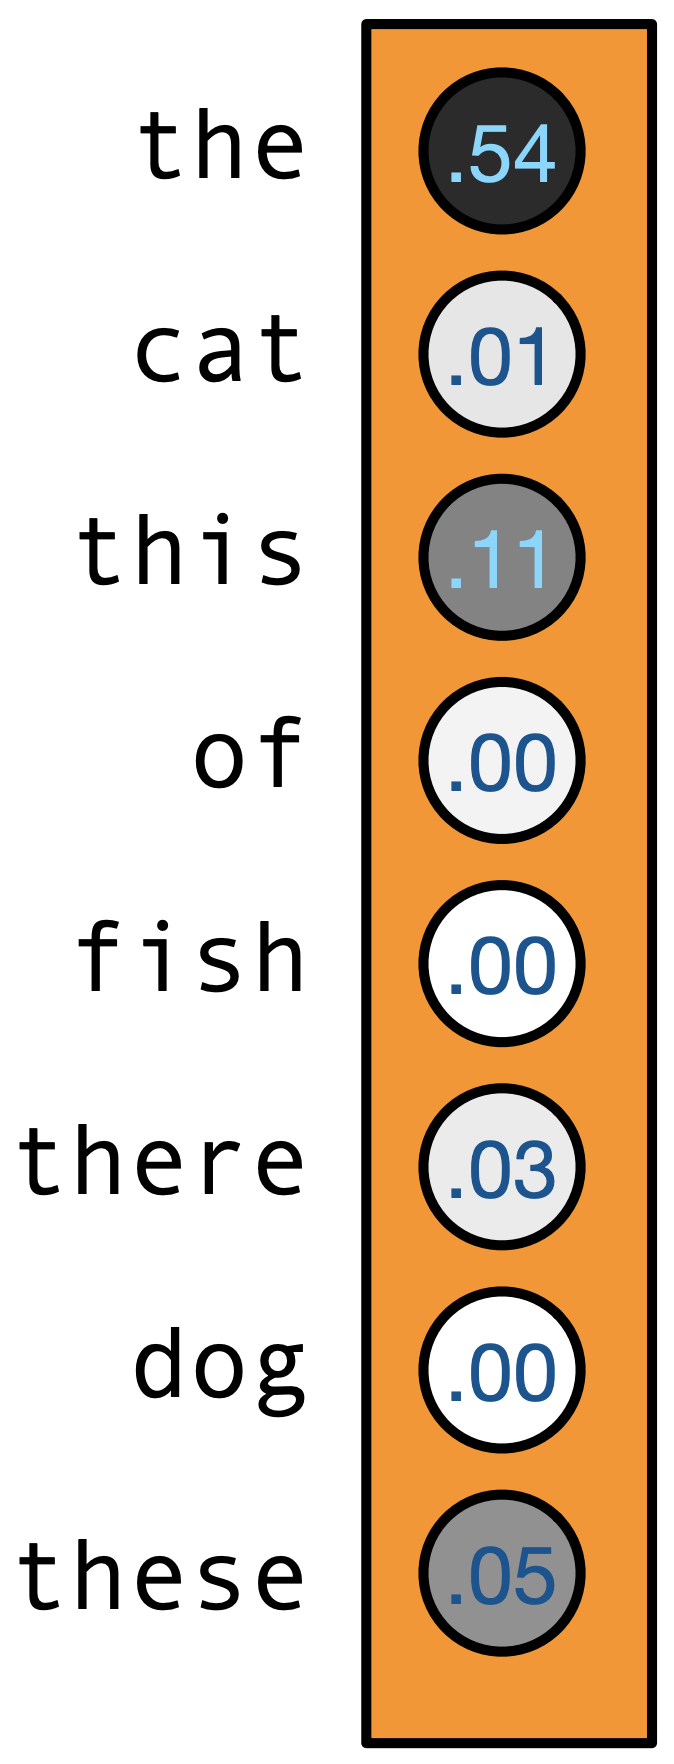
\includegraphics[height=4.5cm, valign=c]{assets/monte_carlo} \right)$
    % 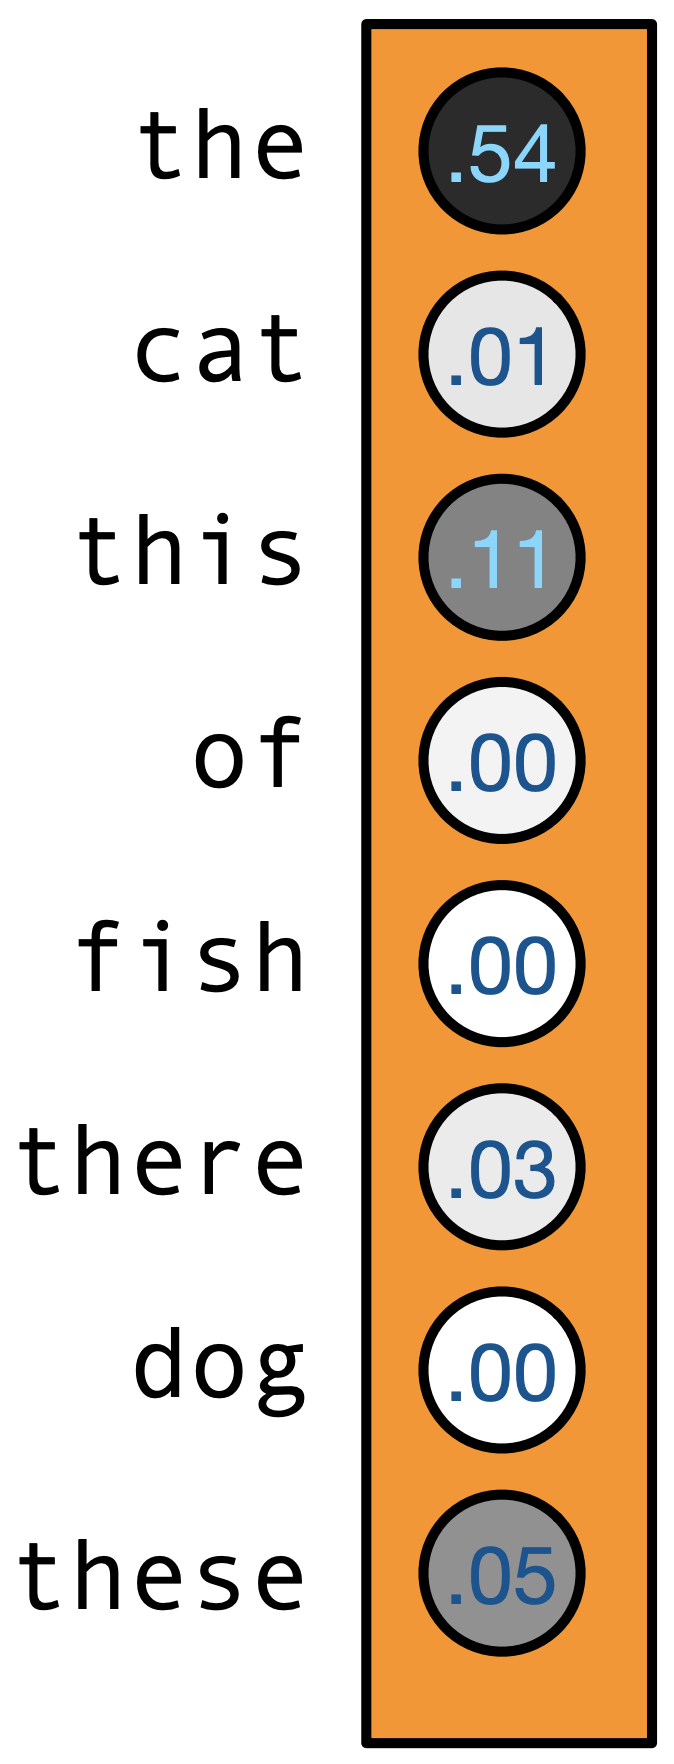
\includegraphics[height=4.5cm, valign=c]{assets/monte_carlo}
  \end{figure}
  \begin{itemize}
    \item Why not sample $n$ words based on their probabilities?
    \item Adds more diversity to beam search results
  \end{itemize}
\end{frame}

\begin{frame}
\frametitle{Ensembling}
\begin{figure}
  \centering
  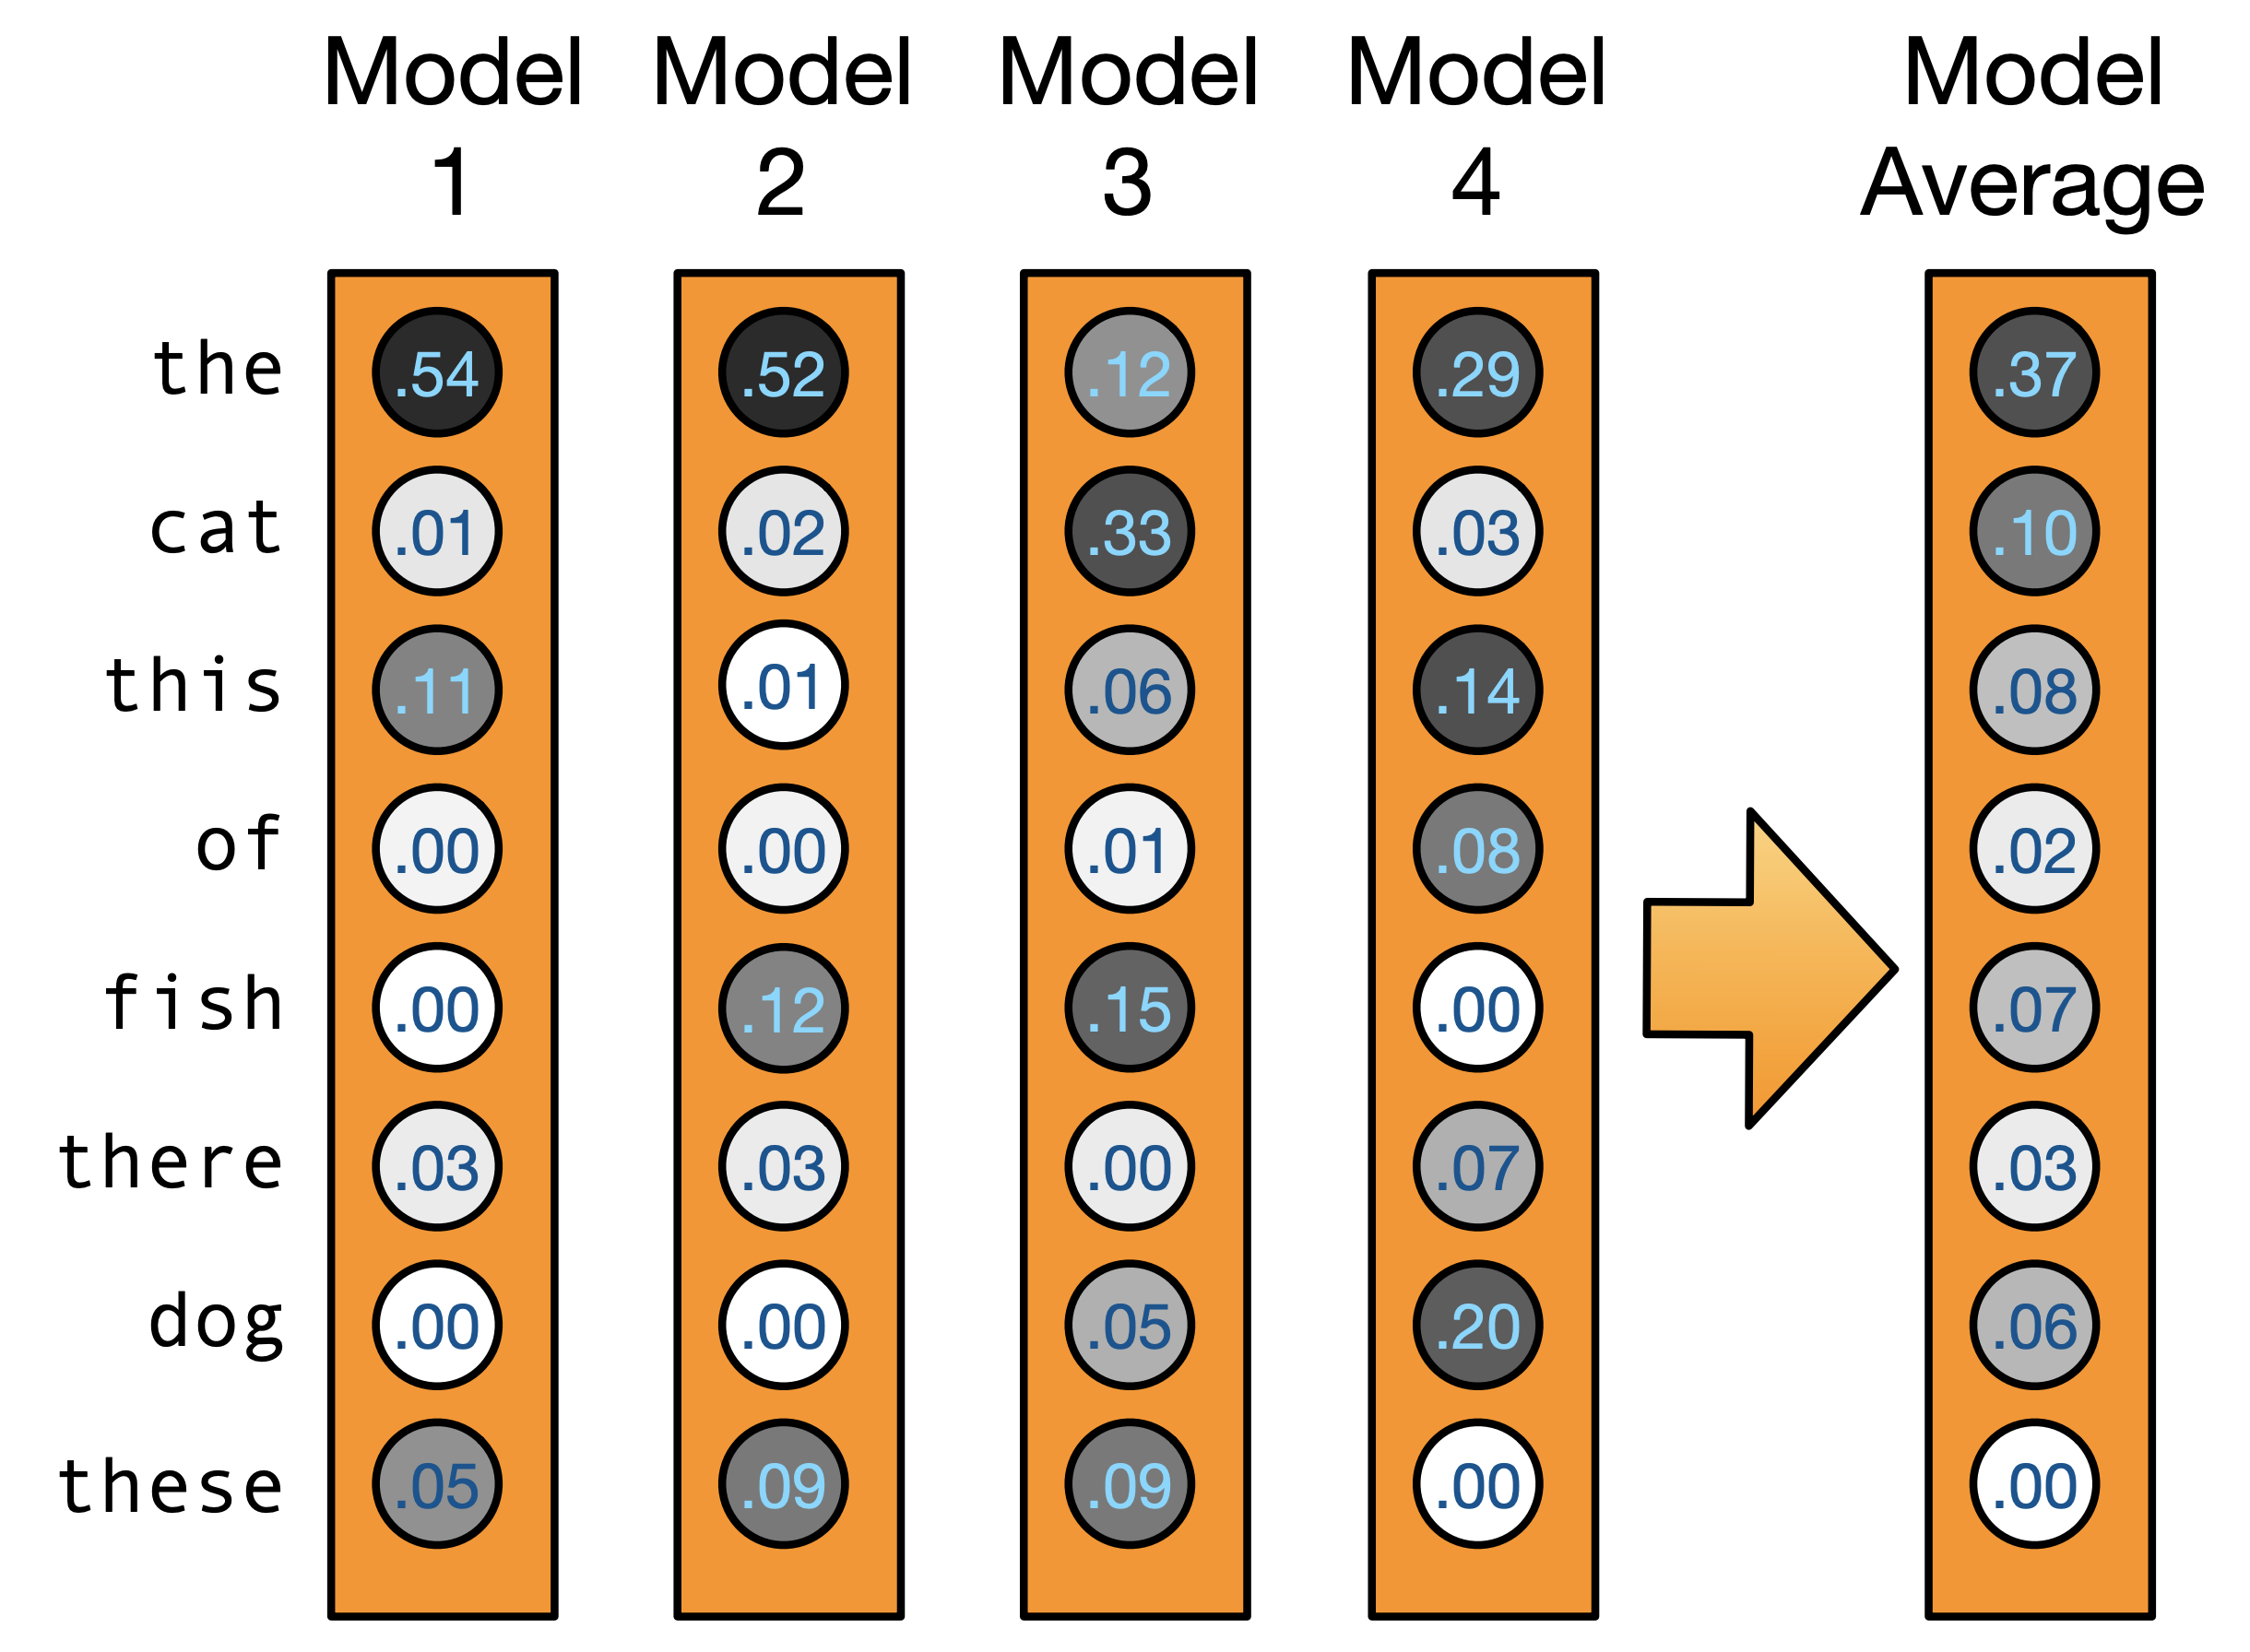
\includegraphics[width=7cm, valign=c]{assets/ensemble}
\end{figure}
\begin{itemize}
  \item Why not average different models?
  \item Random initialization leads to different local solutions
  \item Could also use model dumps from different iterations
\end{itemize}
\end{frame}


%%%%%%%%%%%%%%%%%%%%%%%%%%%%%%%%%%%%%%%%%%%%%%%%%%%%%%%%%%%%%%%%%%%%%%%%%%%%%%%%
\section{Modeling Recurrent Relations}

\begin{frame}
\frametitle{Vanilla RNNs}
\begin{equation*}
  h_t = \tanh \left( \overbrace{W_{ih} x_t + b_{ih}}^{input} + \underbrace{W_{hh} h_{t-1} + b_{hh}}_{hidden} \right)
\end{equation*}
\begin{itemize}
  \item $h_t$ is the hidden state at time $t$
  \item $x_t$ is the input at time $t$
  \item $h_{t-1}$ is the previous hidden state
  \item $h_0$ is initialized to $\mathbf{0}$

\end{itemize}
\end{frame}

\begin{frame}
\frametitle{Long Short Term Memory (LSTM)}
\begin{equation*}
  \begin{split}
  \text{Gates} \rightarrow & \begin{cases}
  \begin{array}{ll}
              i_t = \sigma(W_{ii} x_t + b_{ii} + W_{hi} h_{t-1} + b_{hi}) \\
              f_t = \sigma(W_{if} x_t + b_{if} + W_{hf} h_{t-1} + b_{hf}) \\
              o_t = \sigma(W_{io} x_t + b_{io} + W_{ho} h_{t-1} + b_{ho}) \\
              g_t = \tanh(W_{ig} x_t + b_{ig} + W_{hg} h_{t-1} + b_{hg}) \\
  \end{array}
  \end{cases} \\
  \text{Outputs} \rightarrow & \begin{cases}
  \begin{array}{ll}
              c_t = f_t \odot c_{t-1} + i_t \odot g_t \\
              h_t = o_t \odot \tanh(c_t) \\
  \end{array}
\end{cases}
\end{split}
\end{equation*}

\begin{itemize}
  \item $h_t$ is the hidden state at time $t$
  \item $c_t$ is the cell state at time $t$
  \item $x_t$ is the input at time $t$

\end{itemize}
\end{frame}

\begin{frame}
\frametitle{Gated Recurrent Units (GRU)}
\begin{equation*}
  \begin{split}
  \text{Gates} \rightarrow & \begin{cases}
  \begin{array}{ll}
    r_t = \sigma(W_{ir} x_t + b_{ir} + W_{hr} h_{(t-1)} + b_{hr}) \\
    z_t = \sigma(W_{iz} x_t + b_{iz} + W_{hz} h_{(t-1)} + b_{hz}) \\
    n_t = \tanh(W_{in} x_t + b_{in} + r_t \odot (W_{hn} h_{(t-1)}+ b_{hn})) \\
  \end{array}
  \end{cases} \\
  \text{Outputs} \rightarrow & \begin{cases}
  \begin{array}{ll}
            h_t = (1 - z_t) \odot n_t + z_t \odot h_{(t-1)}
  \end{array}
\end{cases}
\end{split}
\end{equation*}
\begin{itemize}
  \item $h_t$ is the hidden state at time $t$
  \item $x_t$ is the input at time $t$
\end{itemize}

\end{frame}

\begin{frame}
\frametitle{Aside: Different Perspectives on Deep Recurrent Models}
  % insert koehn deep model nn-lm slide 37
  \begin{itemize}
    \item So far we've only seen Left to Right Sequencing
  \end{itemize}
  \begin{figure}
    \centering
    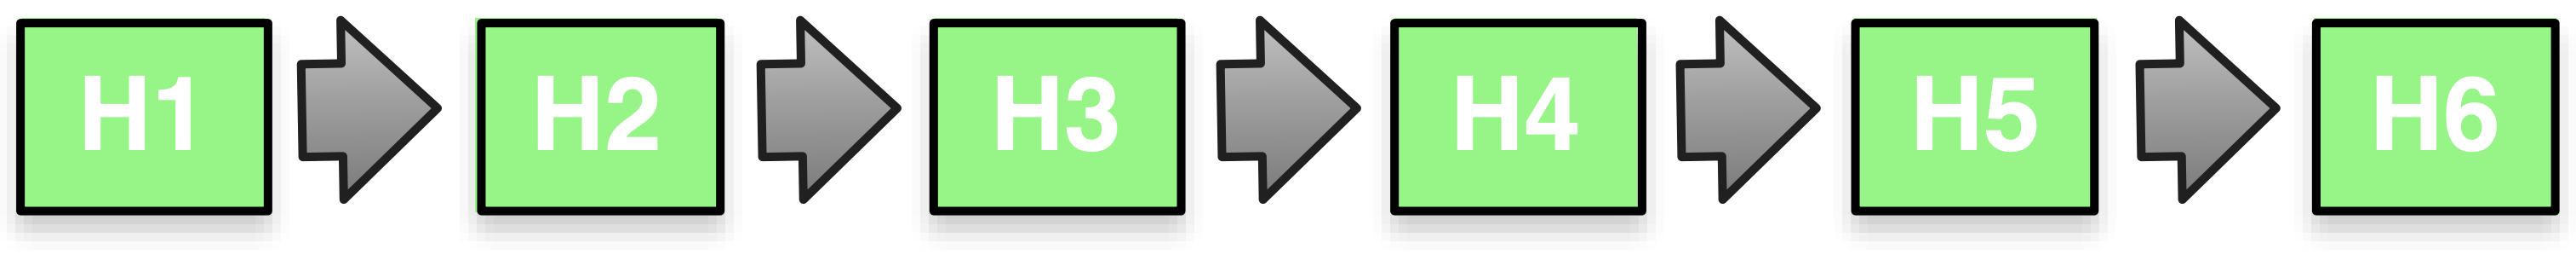
\includegraphics[width=10cm]{assets/L2R}
  \end{figure}
  \pause
  \begin{itemize}
    \item Why not Right to Left?
  \end{itemize}
  \begin{figure}
    \centering
    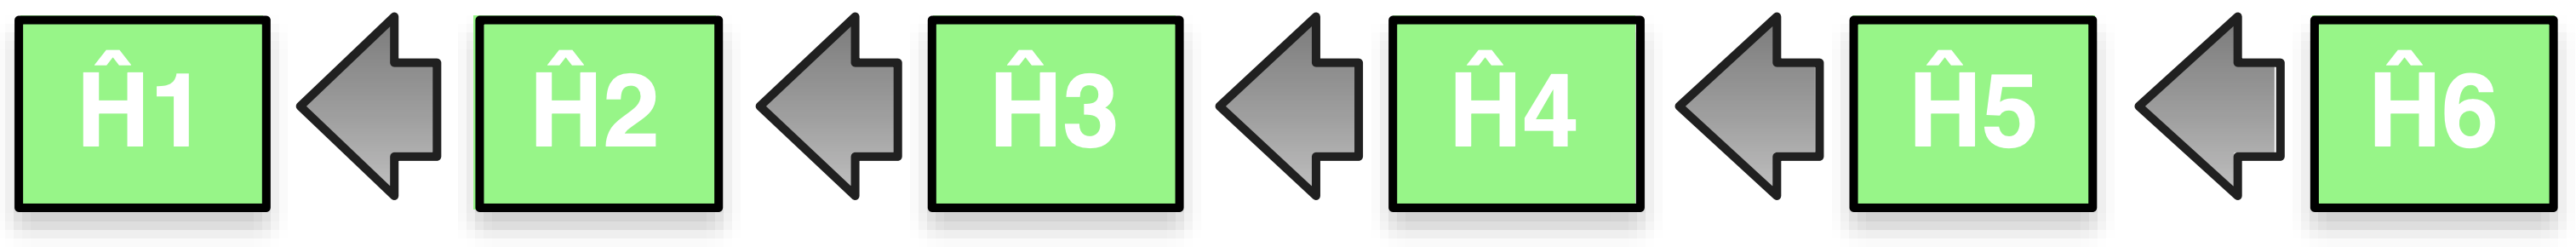
\includegraphics[width=10cm]{assets/R2L}
  \end{figure}
\end{frame}


\begin{frame}
\frametitle{Aside: Different Perspectives on Deep Recurrent Models}
\begin{figure}
  \centering
  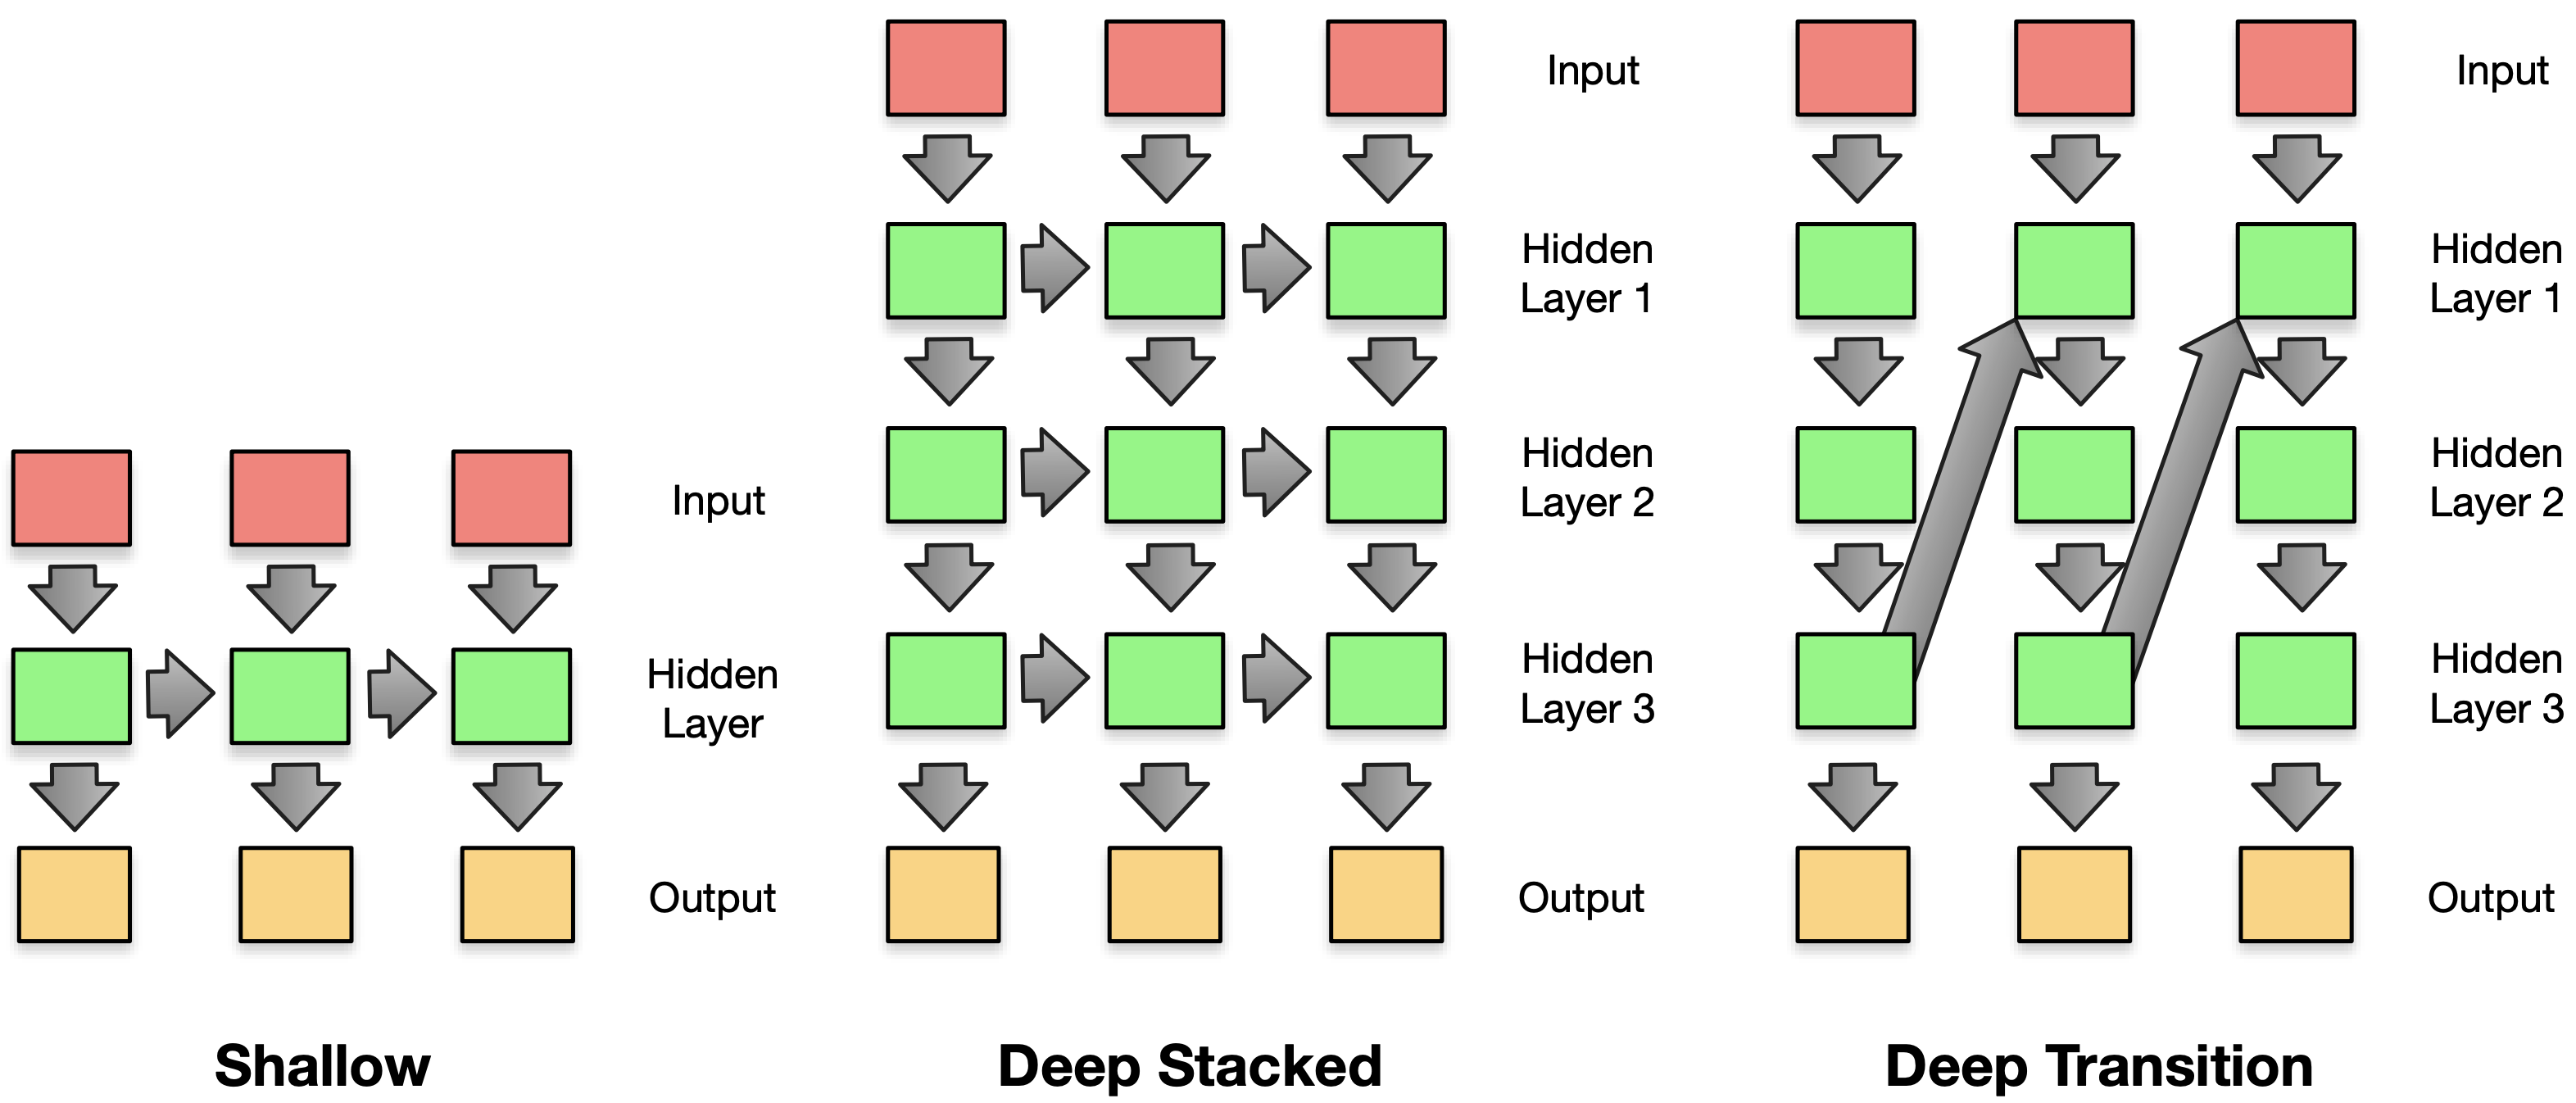
\includegraphics[width=10cm]{assets/deep_models}
\end{figure}
\begin{itemize}
  \item Experiment with different stacking techniques
\end{itemize}
\end{frame}

\begin{frame}
\frametitle{Alternating Recurrent Directions}
\begin{figure}
  \centering
  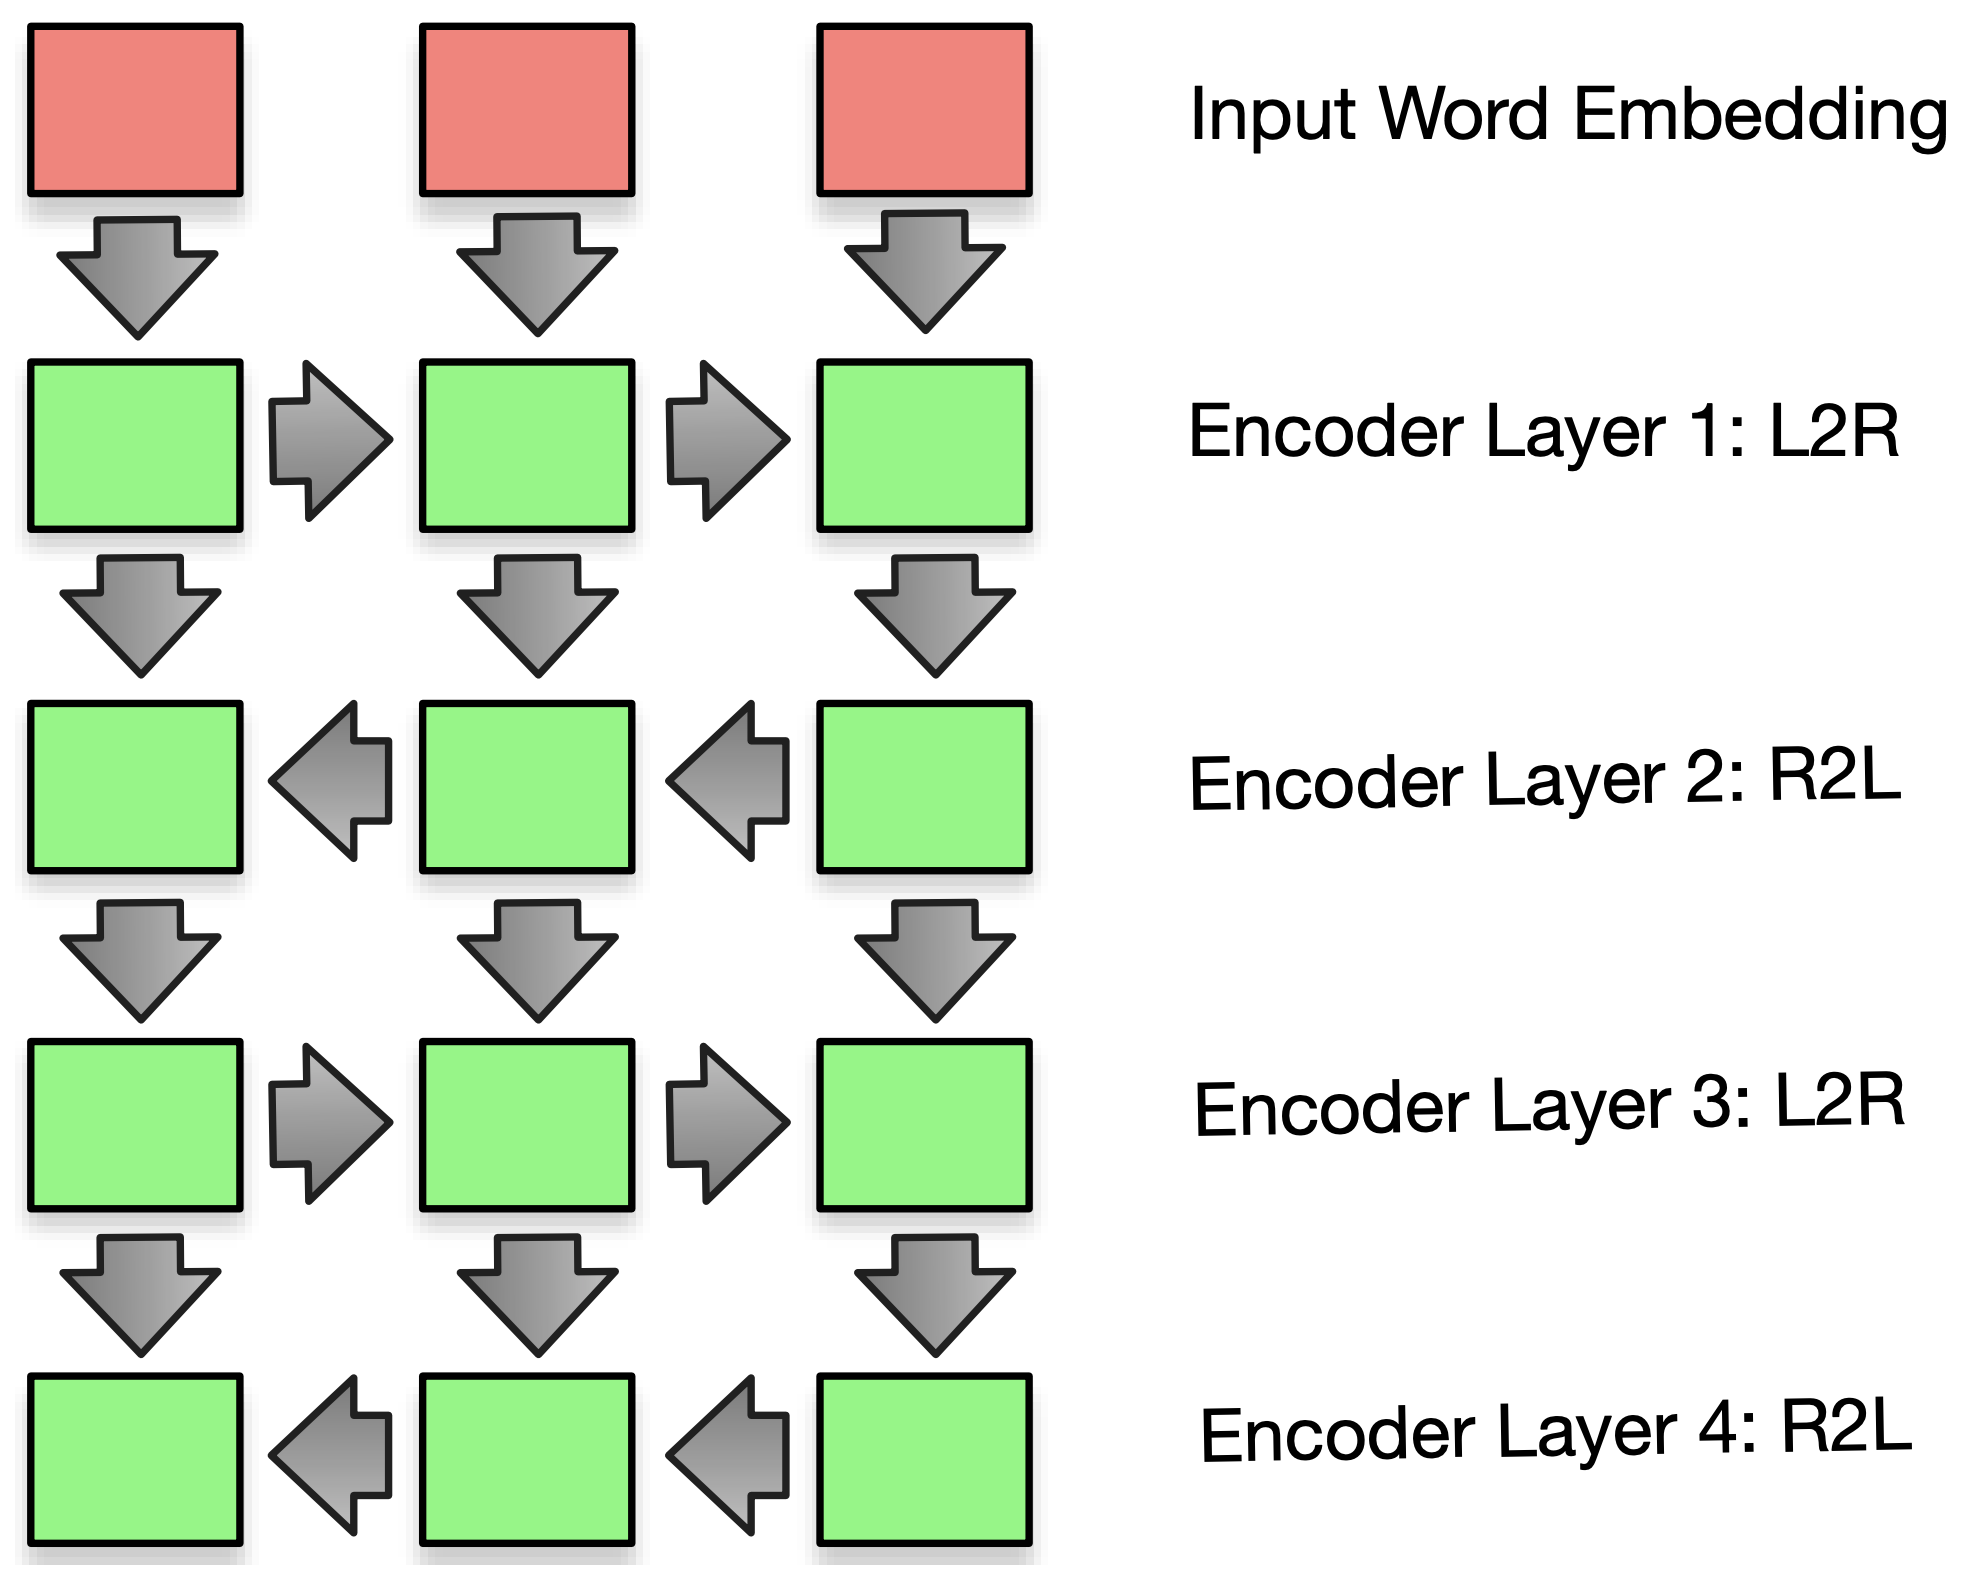
\includegraphics[width=9cm]{assets/alternate_stacked}
\end{figure}
\end{frame}

\begin{frame}
\frametitle{Bidirectional Sequence Modeling}
\begin{figure}
  \centering
  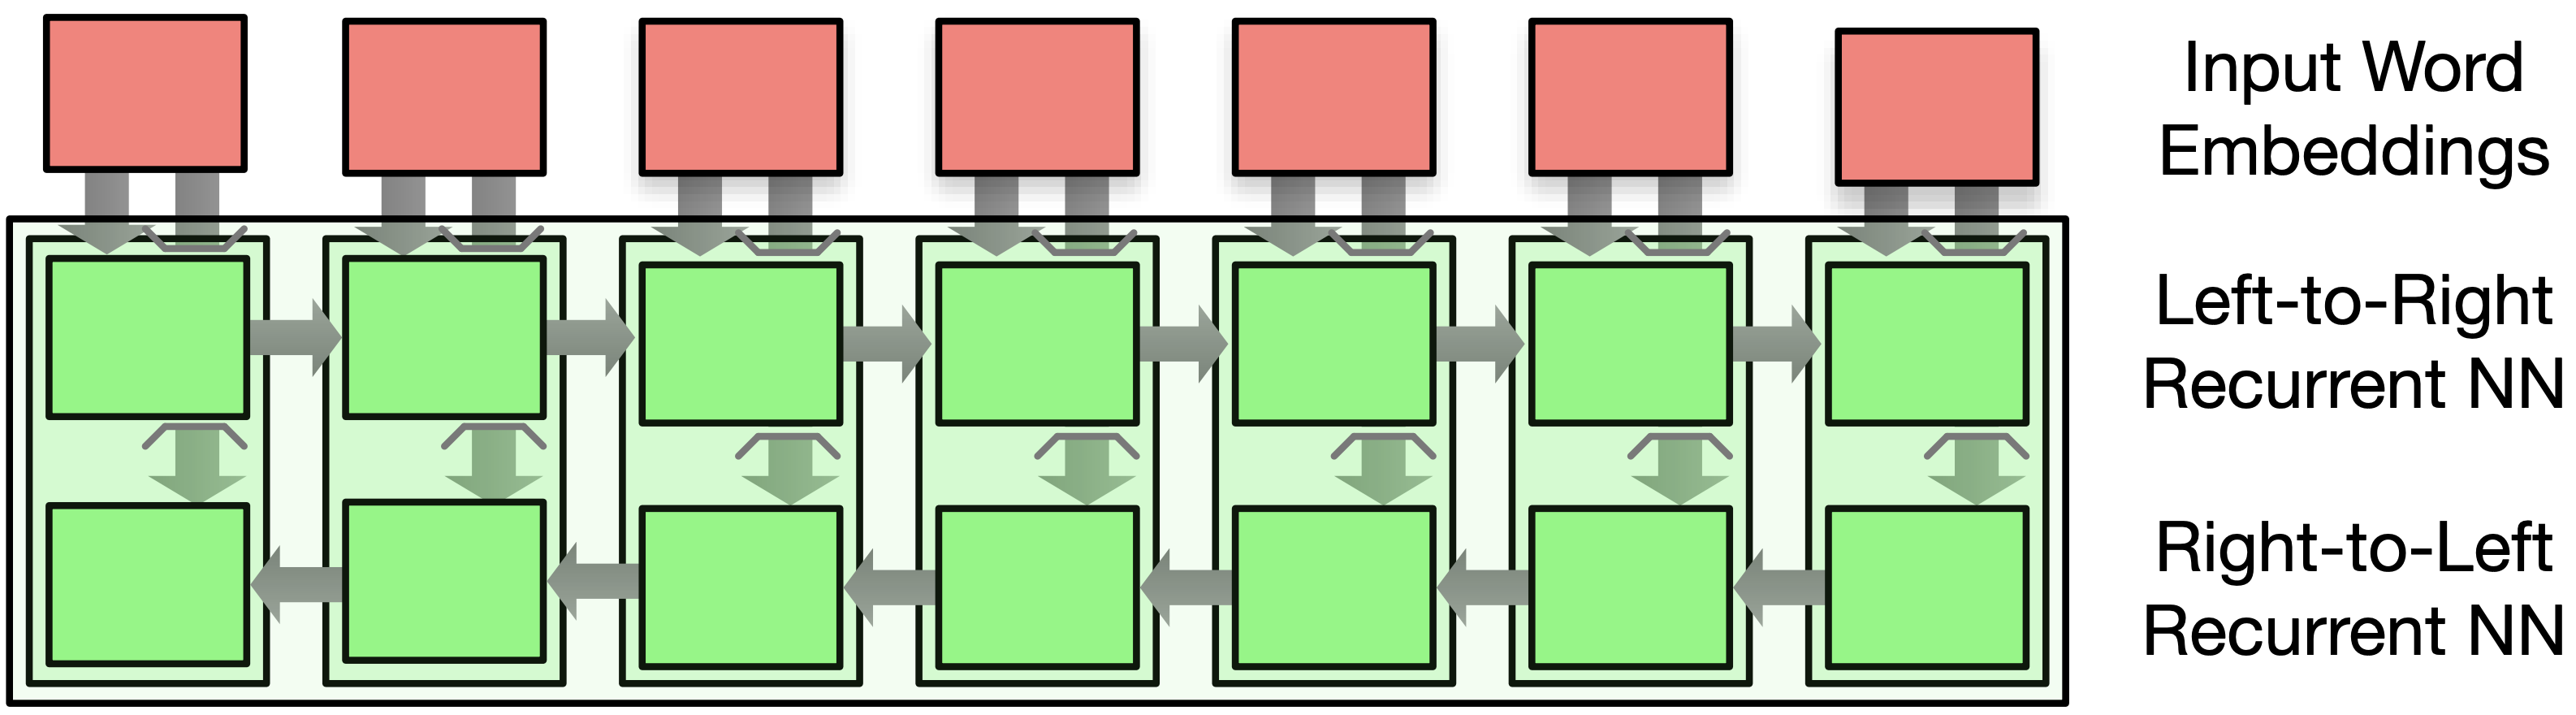
\includegraphics[width=10cm]{assets/bidirectional}
\end{figure}
\begin{itemize}
  \item Can capture both left and right context
  \item Implementation usually concatenates RNN states
\end{itemize}
\end{frame}



\begin{frame}
\frametitle{Aside: Dimensionality of Inputs and Outputs (Batch First)}

\begin{center}
\begin{tabular}{l|C{2.5cm}|C{2.5cm}|C{2.5cm}}
\toprule
\multicolumn{1}{c}{Type} &  \multicolumn{1}{c}{RNN} &  \multicolumn{1}{c}{LSTM} &  \multicolumn{1}{c}{GRU} \\
\midrule
In            & $B, L, H_{in}$              & $B, L, H_{in}$              & $B, L, H_{in}$ \\
\midrule
$h_{t-1}$ & $N_L \cdot N_D, B, H_{out}$ & $N_L \cdot N_D, B, H_{out}$ & $N_L \cdot N_D, B, H_{out}$ \\
$c_{t-1}$   & - & $N_L \cdot N_D, B, H_{out}$      & - \\
\midrule
$h_t$   & $N_L \cdot N_D, B, H_{out}$ & $N_L \cdot N_D, B, H_{out}$ & $N_L \cdot N_D, B, H_{out}$ \\
$c_t$     & - & $N_L \cdot N_D, B, H_{out}$ & - \\
\midrule
Out & $B, L, N_D \cdot H_{out}$   & $B, L, N_D \cdot H_{out}$   & $B, L, N_D \cdot H_{out}$ \\
\bottomrule
\end{tabular}
\end{center}

\begin{itemize}
  \item $B$ is the batch size
  \item $L$ is the sequence length
  \item $N_D$ is the number of directions
  \item $N_L$ is the number of layers
  \item $H_{in}, H_{out}$ are the input and hidden size
\end{itemize}
\end{frame}

\begin{frame}
\frametitle{Aside: The Influence of Padding in RNNs}
  \begin{itemize}
    \item Assume the embedding $E\left[ \textcolor{WildStrawberry}{\langle \texttt{PAD} \rangle} \right] = \mathbf{0}$
    \item Are we safe? \pause \textbf{NO!}
    \item Because of the bias term, zero input does not result in a zero output
    \begin{itemize}
      \item This alters the hidden state being passed onto the next iteration
    \end{itemize}
    \item Don't even think about the mess bidirectionals become...
    \item \textbf{Question:} Does this mean we learn the amount of padding for a given sequence?
  \end{itemize}
\end{frame}

%%%%%%%%%%%%%%%%%%%%%%%%%%%%%%%%%%%%%%%%%%%%%%%%%%%%%%%%%%%%%%%%%%%%%%%%%%%%%%%%

\section{Applications to Column Segmentation}

\begin{frame}
  \frametitle{Applications to Column Segmentation}
  \begin{figure}
    \centering
    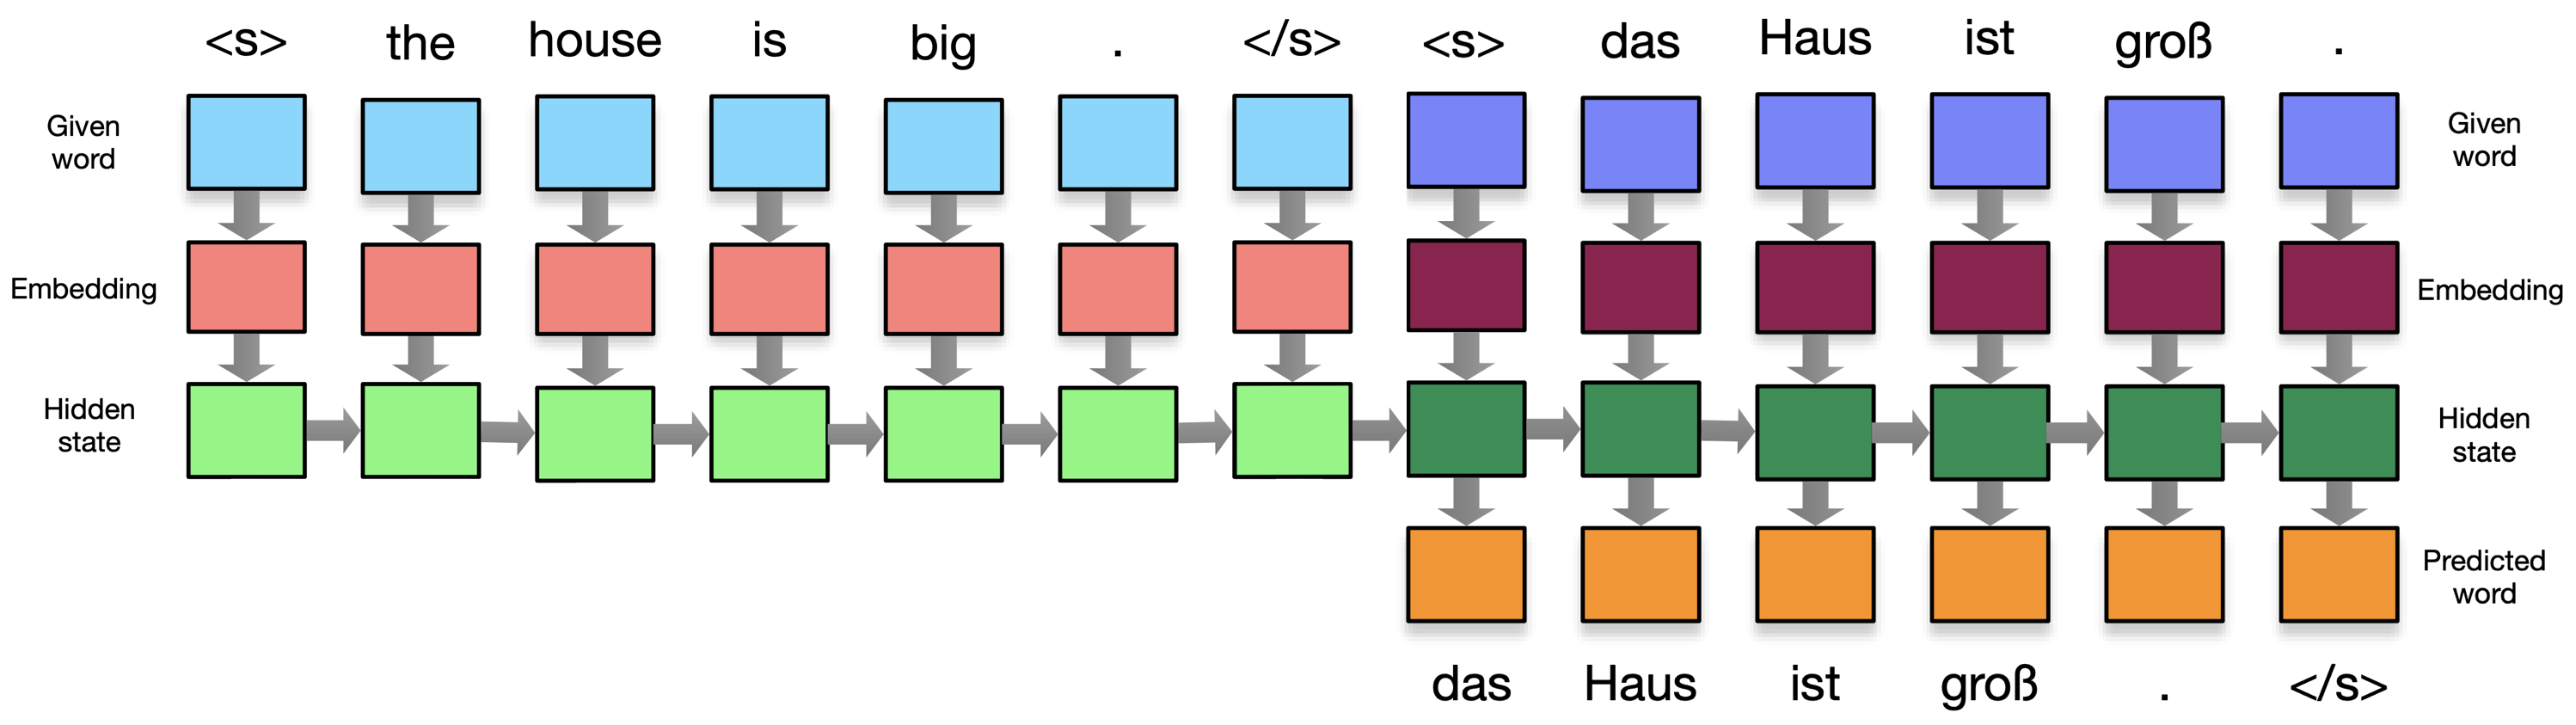
\includegraphics[width=10cm, valign=c]{assets/enc-dec}
  \end{figure}
  % add picture from notebook
  \begin{figure}
    \centering
    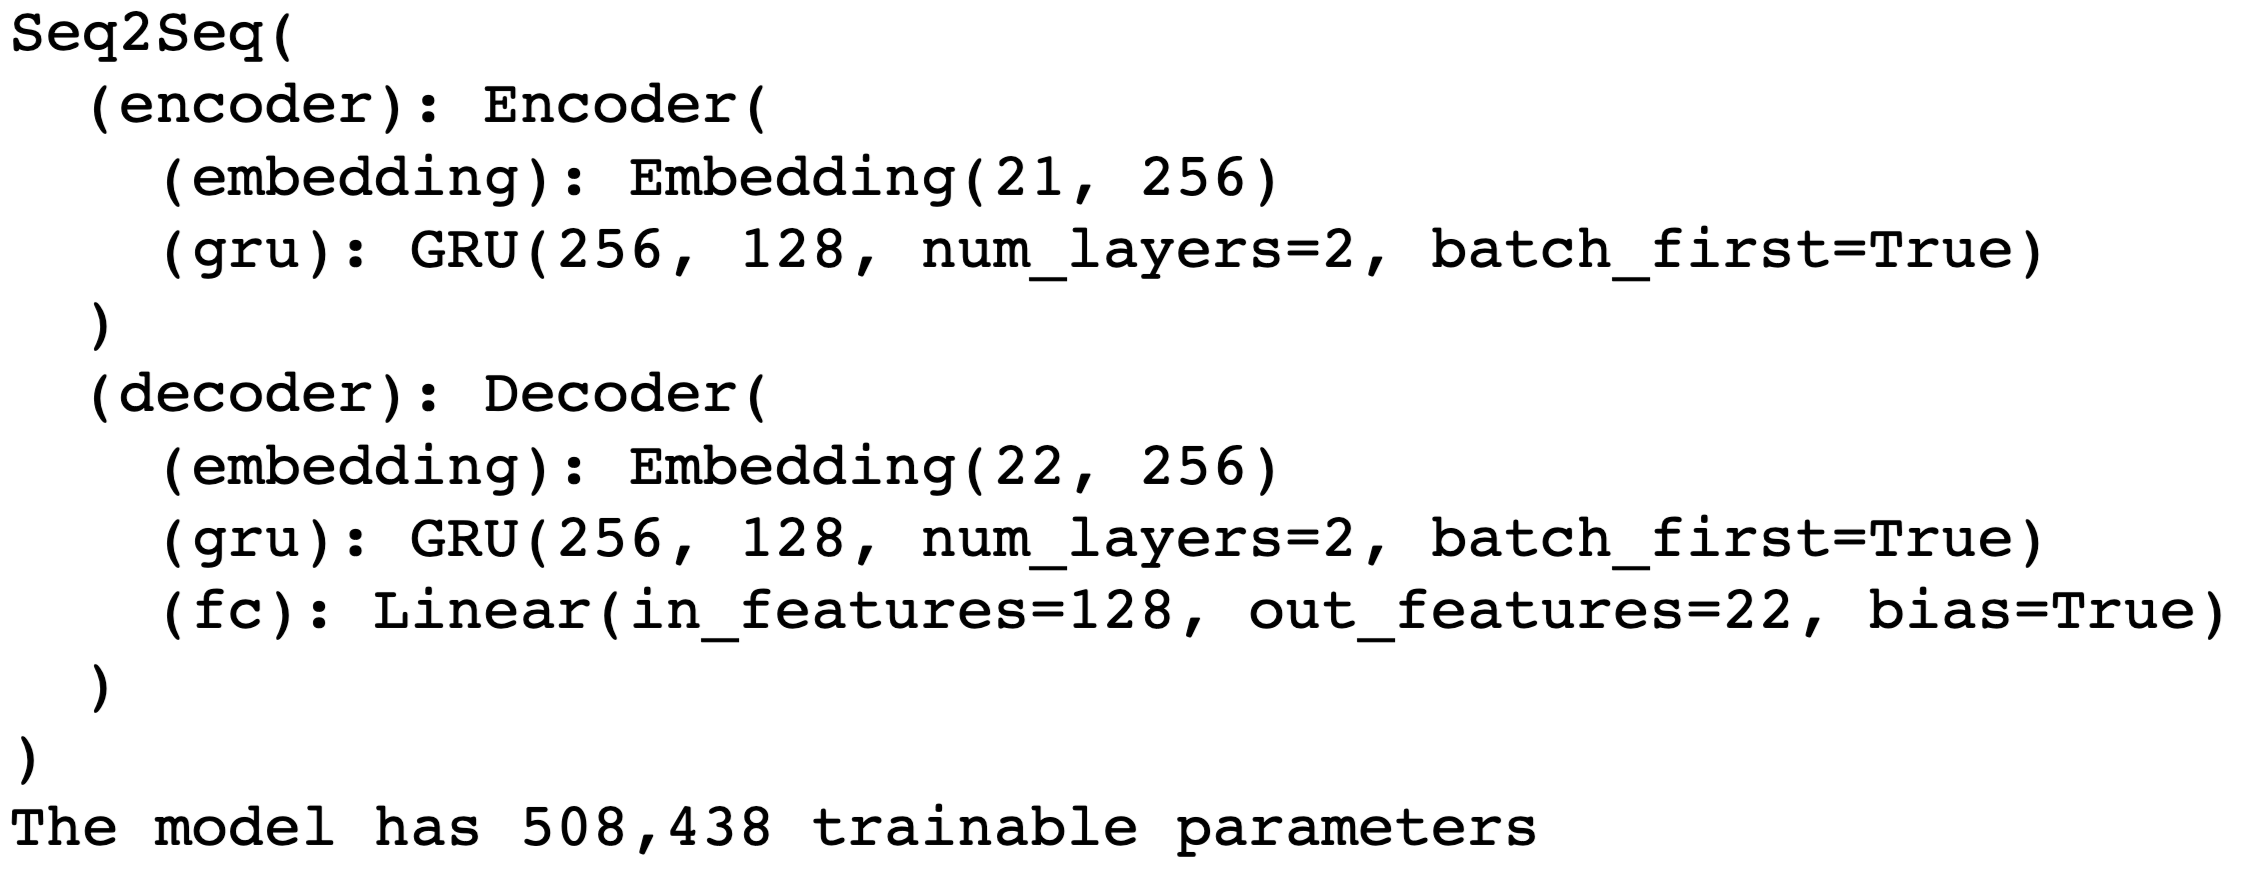
\includegraphics[width=10cm, valign=c]{assets/col-seq2seq}
  \end{figure}
\end{frame}

\begin{frame}
  \frametitle{Column Segmentation: Throw away the decoder}
  \begin{itemize}
    \item Just use an encoder, with an output layer
    \item For every token, predict if we should insert a $\textcolor{WildStrawberry}{\langle \texttt{SEG} \rangle}$
    \item No longer have to learn the actual sequence
  \end{itemize}
  \begin{figure}
    \centering
    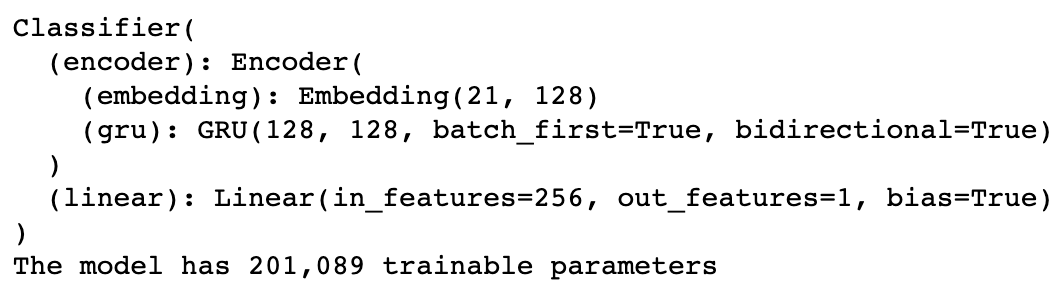
\includegraphics[width=10cm, valign=c]{assets/col-encoder}
  \end{figure}
\end{frame}

\begin{frame}
  \frametitle{Independent Row: Training Labels}
  \begin{itemize}
    \item Labels are now binary vectors, where $x_i = 1$ implies that there is a $\textcolor{WildStrawberry}{\langle \texttt{SEG} \rangle}$
      between $x_i$ and $x_{i+1}$
  \end{itemize}
  \vspace{5mm}
  \begin{equation*}
    \centering
    \textcolor{ForestGreen}{
    \begin{array}{cccccccc}
      \texttt{Less} & \texttt{imputed} & \texttt{interest} & {} & \texttt{(} & \texttt{174,862.64} & \texttt{)} \\
      \textcolor{Fuchsia}{\texttt{0}} & \textcolor{Fuchsia}{\texttt{0}} & \textcolor{Fuchsia}{\texttt{\textbf{1}}} & {} & \textcolor{Fuchsia}{\texttt{0}} & \textcolor{Fuchsia}{\texttt{0}} & \textcolor{Fuchsia}{\texttt{0}} \\
      \texttt{Less} & \texttt{imputed} & \texttt{interest} & \textcolor{WildStrawberry}{\langle \texttt{SEG} \rangle} & \texttt{(} & \texttt{174,862.64} & \texttt{)} \\
    \end{array}}
  \end{equation*}
\end{frame}

\begin{frame}
  \frametitle{Independent Row Training Visual}
  \begin{figure}
    \centering
    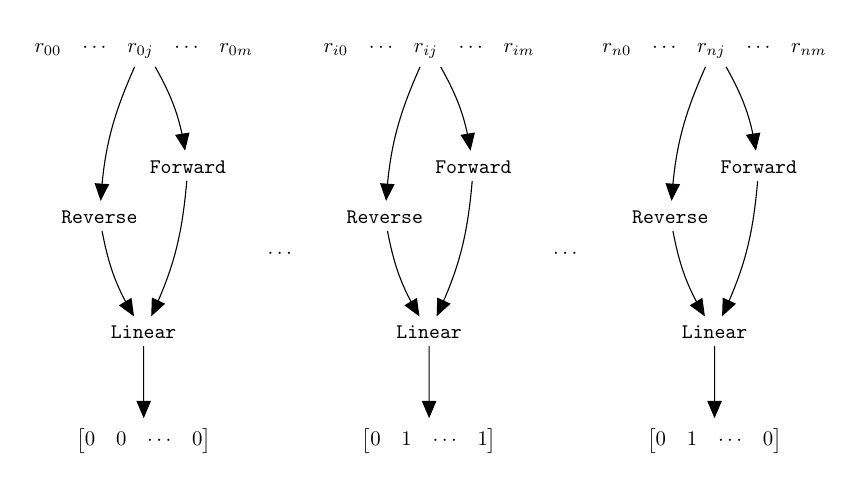
\begin{tikzpicture}[shorten >=1pt,node distance=1cm,on grid,auto, every node/.style={scale=0.75},
      el/.style={inner sep=2pt, align=left, sloped}]

      \node[] (r0) {$\begin{matrix} r_{00} & \cdots & r_{0j} & \cdots & r_{0m} \end{matrix}$};
      \node[] (for0) [below=of r0, yshift=-0.7cm, xshift=0.75cm] {$\texttt{Forward}$};
      \node[] (rev0) [below=of r0, yshift=-1.55cm, xshift=-0.75cm] {$\texttt{Reverse}$};

      \node[] (rnn1) [right=of r0, xshift=1cm, yshift=-3.5cm] {$\cdots$};

      \node[] (r1) [right=of r0, xshift=3.5cm] {$\begin{matrix} r_{i0} & \cdots & r_{ij} & \cdots & r_{im} \end{matrix}$};
      \node[] (for1) [below=of r1, yshift=-0.7cm, xshift=0.75cm] {$\texttt{Forward}$};
      \node[] (rev1) [below=of r1, yshift=-1.55cm, xshift=-0.75cm] {$\texttt{Reverse}$};

      \node[] (rnn2) [right=of r1, xshift=1cm, yshift=-3.5cm] {$\cdots$};

      \node[] (rn) [right=of r1, xshift=3.5cm] {$\begin{matrix} r_{n0} & \cdots & r_{nj} & \cdots & r_{nm} \end{matrix}$};
      \node[] (forn) [below=of rn, yshift=-0.7cm, xshift=0.75cm] {$\texttt{Forward}$};
      \node[] (revn) [below=of rn, yshift=-1.55cm, xshift=-0.75cm] {$\texttt{Reverse}$};

      \node[] (linear0) [below=of r0, yshift=-3.5cm] {$\texttt{Linear}$};
      \node[] (linear1) [below=of r1, yshift=-3.5cm] {$\texttt{Linear}$};
      \node[] (linearn) [below=of rn, yshift=-3.5cm] {$\texttt{Linear}$};

      \node[] (out0) [below=of linear0, yshift=-0.5cm] {$\begin{bmatrix} 0 & 0 & \cdots & 0 \end{bmatrix}$};
      \node[] (out1) [below=of linear1, yshift=-0.5cm] {$\begin{bmatrix} 0 & 1 & \cdots & 1 \end{bmatrix}$};
      \node[] (outn) [below=of linearn, yshift=-0.5cm] {$\begin{bmatrix} 0 & 1 & \cdots & 0 \end{bmatrix}$};

      \path[->]
        (r0) edge [bend left=10] node[] {} (for0)
        (r0) edge [bend right=10] node[] {} (rev0)
        (for0) edge [bend left=10] node[] {} (linear0)
        (rev0) edge [bend right=10] node[] {} (linear0)
        (linear0) edge [] node[] {} (out0)

        (r1) edge [bend left=10] node[] {} (for1)
        (r1) edge [bend right=10] node[] {} (rev1)
        (for1) edge [bend left=10] node[] {} (linear1)
        (rev1) edge [bend right=10] node[] {} (linear1)
        (linear1) edge [] node[] {} (out1)

        (rn) edge [bend left=10] node[] {} (forn)
        (rn) edge [bend right=10] node[] {} (revn)
        (forn) edge [bend left=10] node[] {} (linearn)
        (revn) edge [bend right=10] node[] {} (linearn)
        (linearn) edge [] node[] {} (outn);



    \end{tikzpicture}
  \end{figure}
\end{frame}

% \begin{frame}
%   \frametitle{Independent Row: Sample Results}
%   \begin{figure}
%     \centering
%     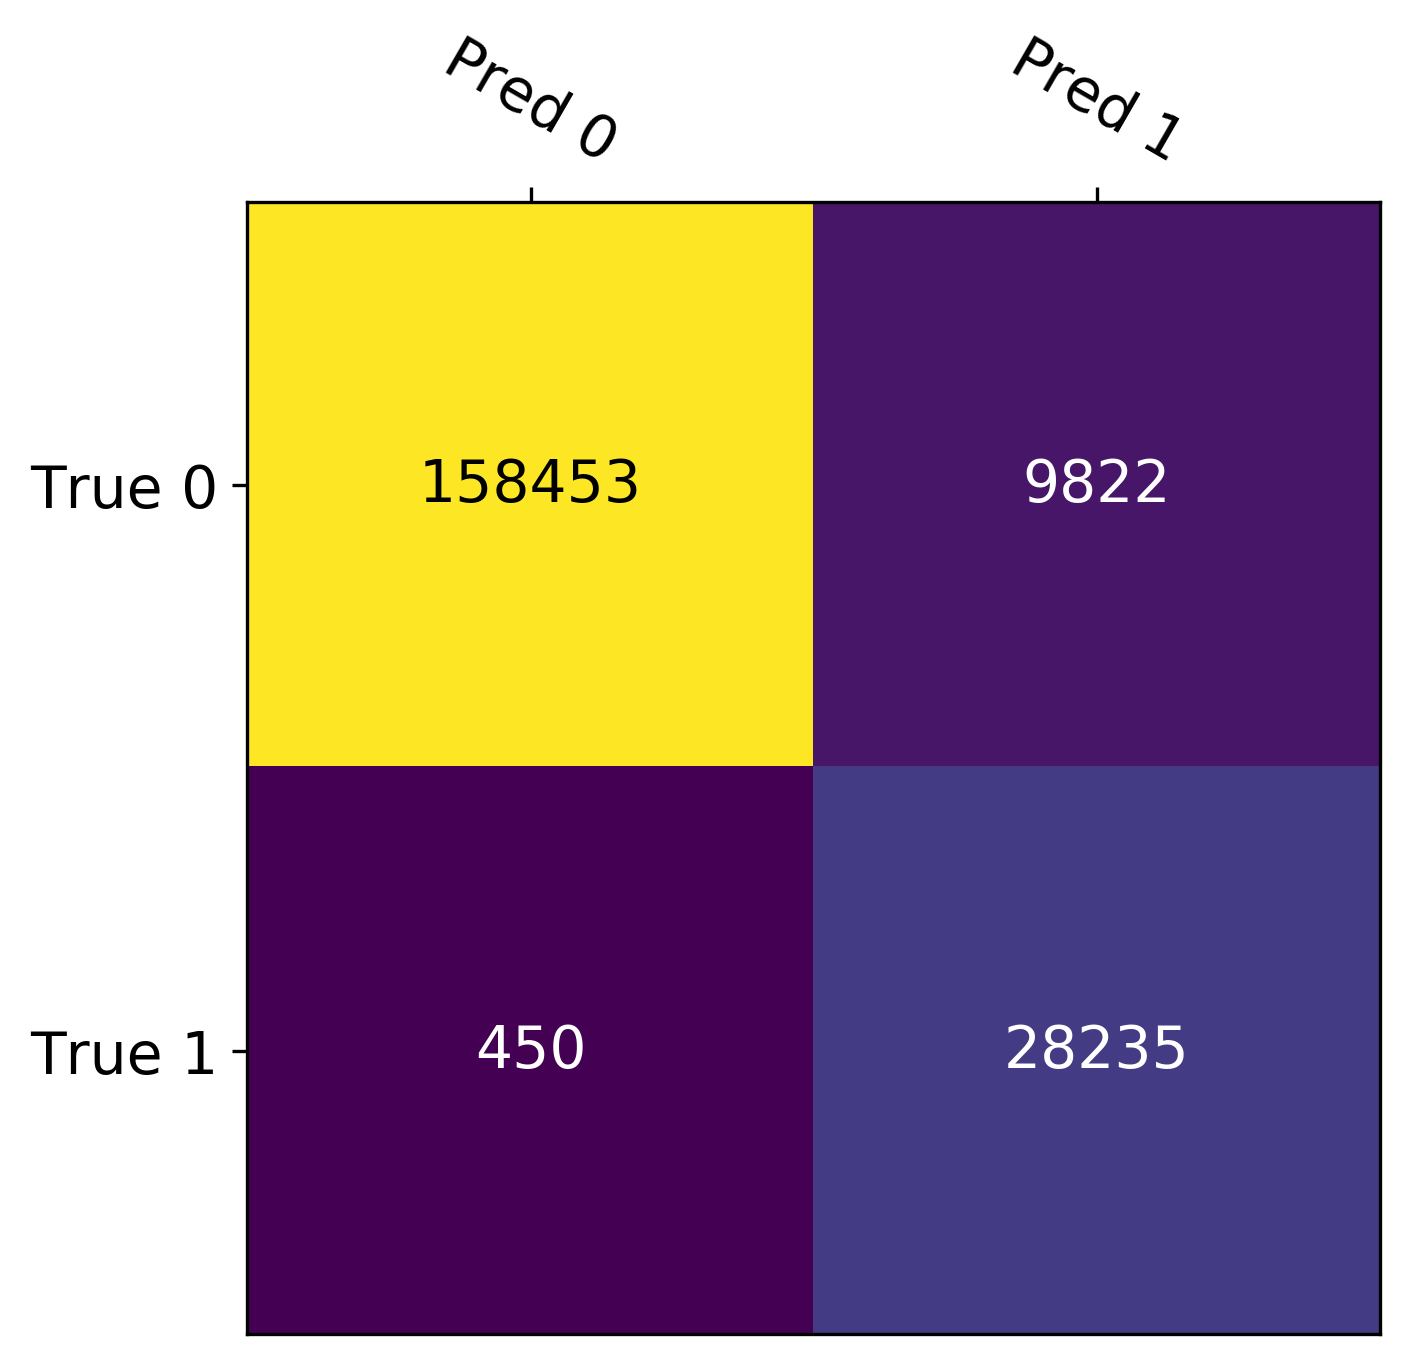
\includegraphics[height=3.75cm, valign=c]{assets/cm}
%     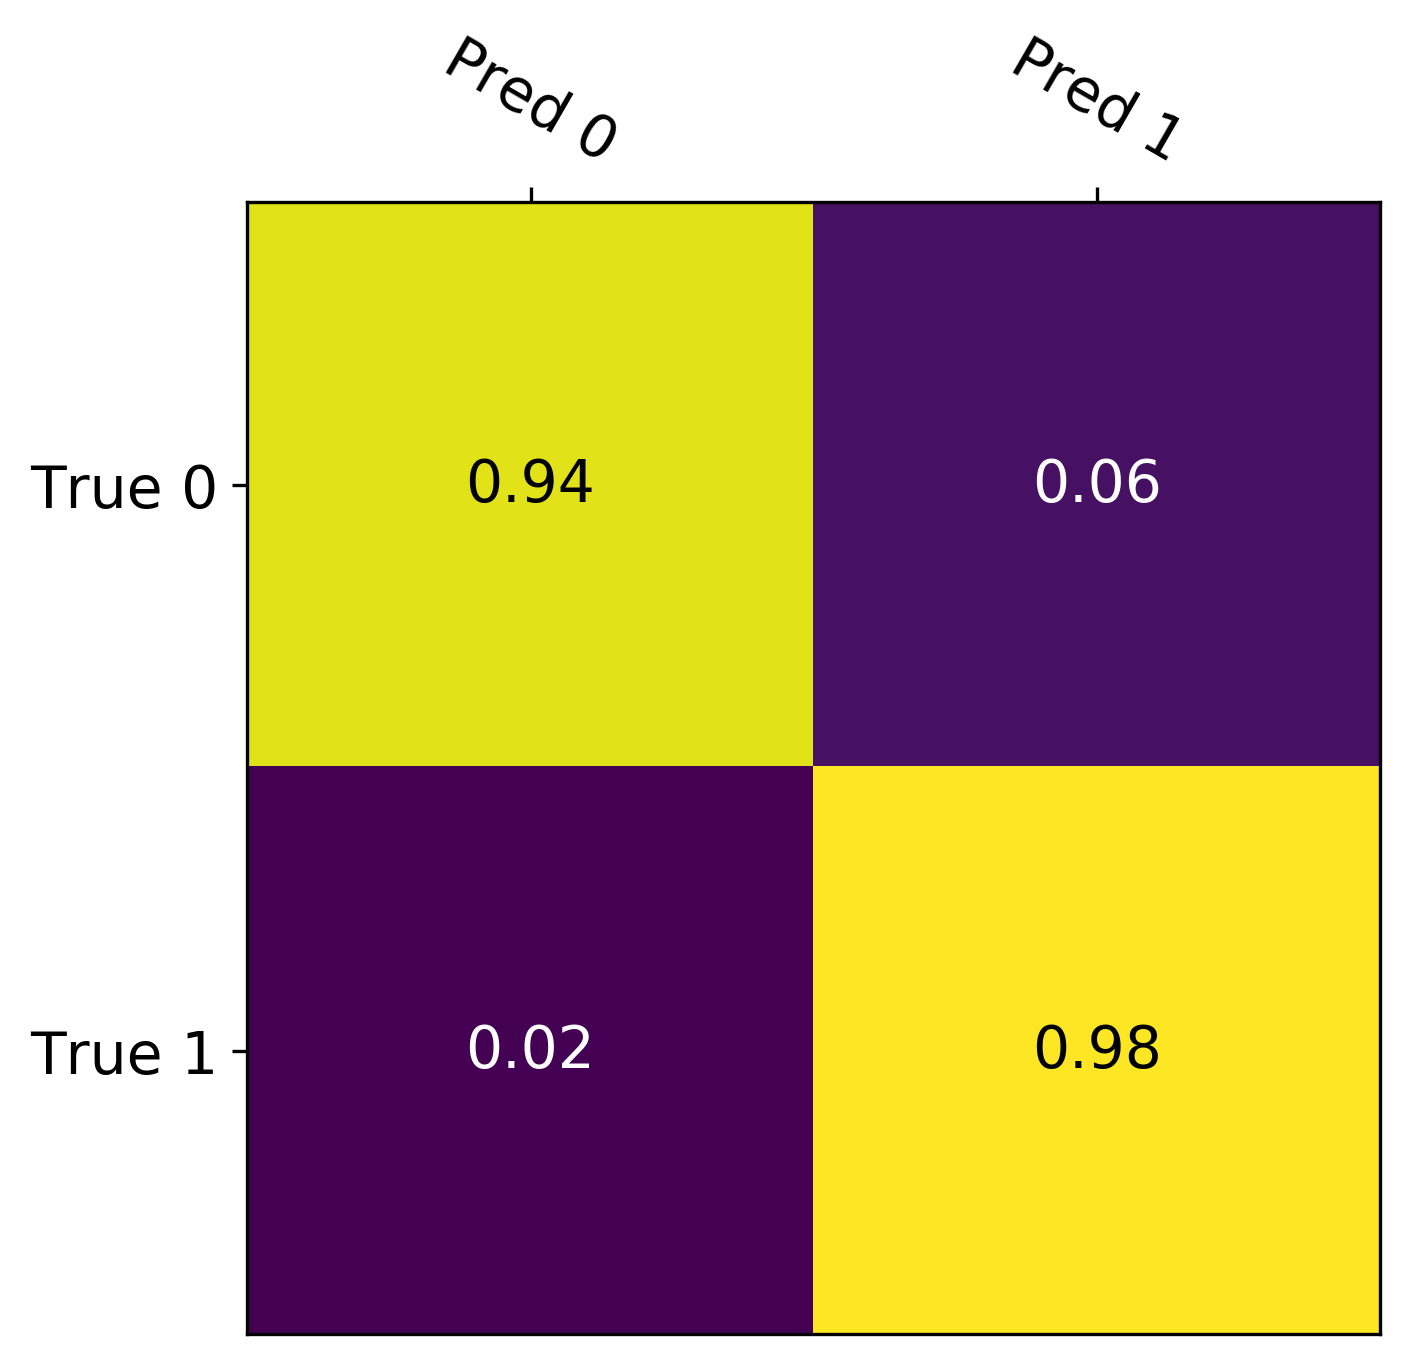
\includegraphics[height=3.75cm, valign=c]{assets/cm_norm}
%   \end{figure}
%   \begin{center}
%     \begin{tabular}{rcccr}
%     \toprule
%     {} &  Precision &  Recall &  F1-Score & Support \\
%     \midrule
%     Label: 0 & $0.99$ & $0.92$ & $0.96$ & $168,275$ \\
%     Label: 1 & $0.67$ & $0.97$ & $0.80$ & $28,685$ \\
%     \midrule
%     accuracy & {} & {} & $0.93$ & $196,960$ \\
%     macro avg & $0.83$ & $0.95$ & $0.88$ & $196,960$ \\
%     weighted avg & $0.95$ & $0.93$ & $0.93$ & $196,960$ \\
%     \bottomrule
%     \end{tabular}
%   \end{center}
%   % something
%   % metrics
%   % graphs
% \end{frame}

\begin{frame}
  \frametitle{Independent Row: Sample Results (Training)}
  \begin{figure}
    \centering
    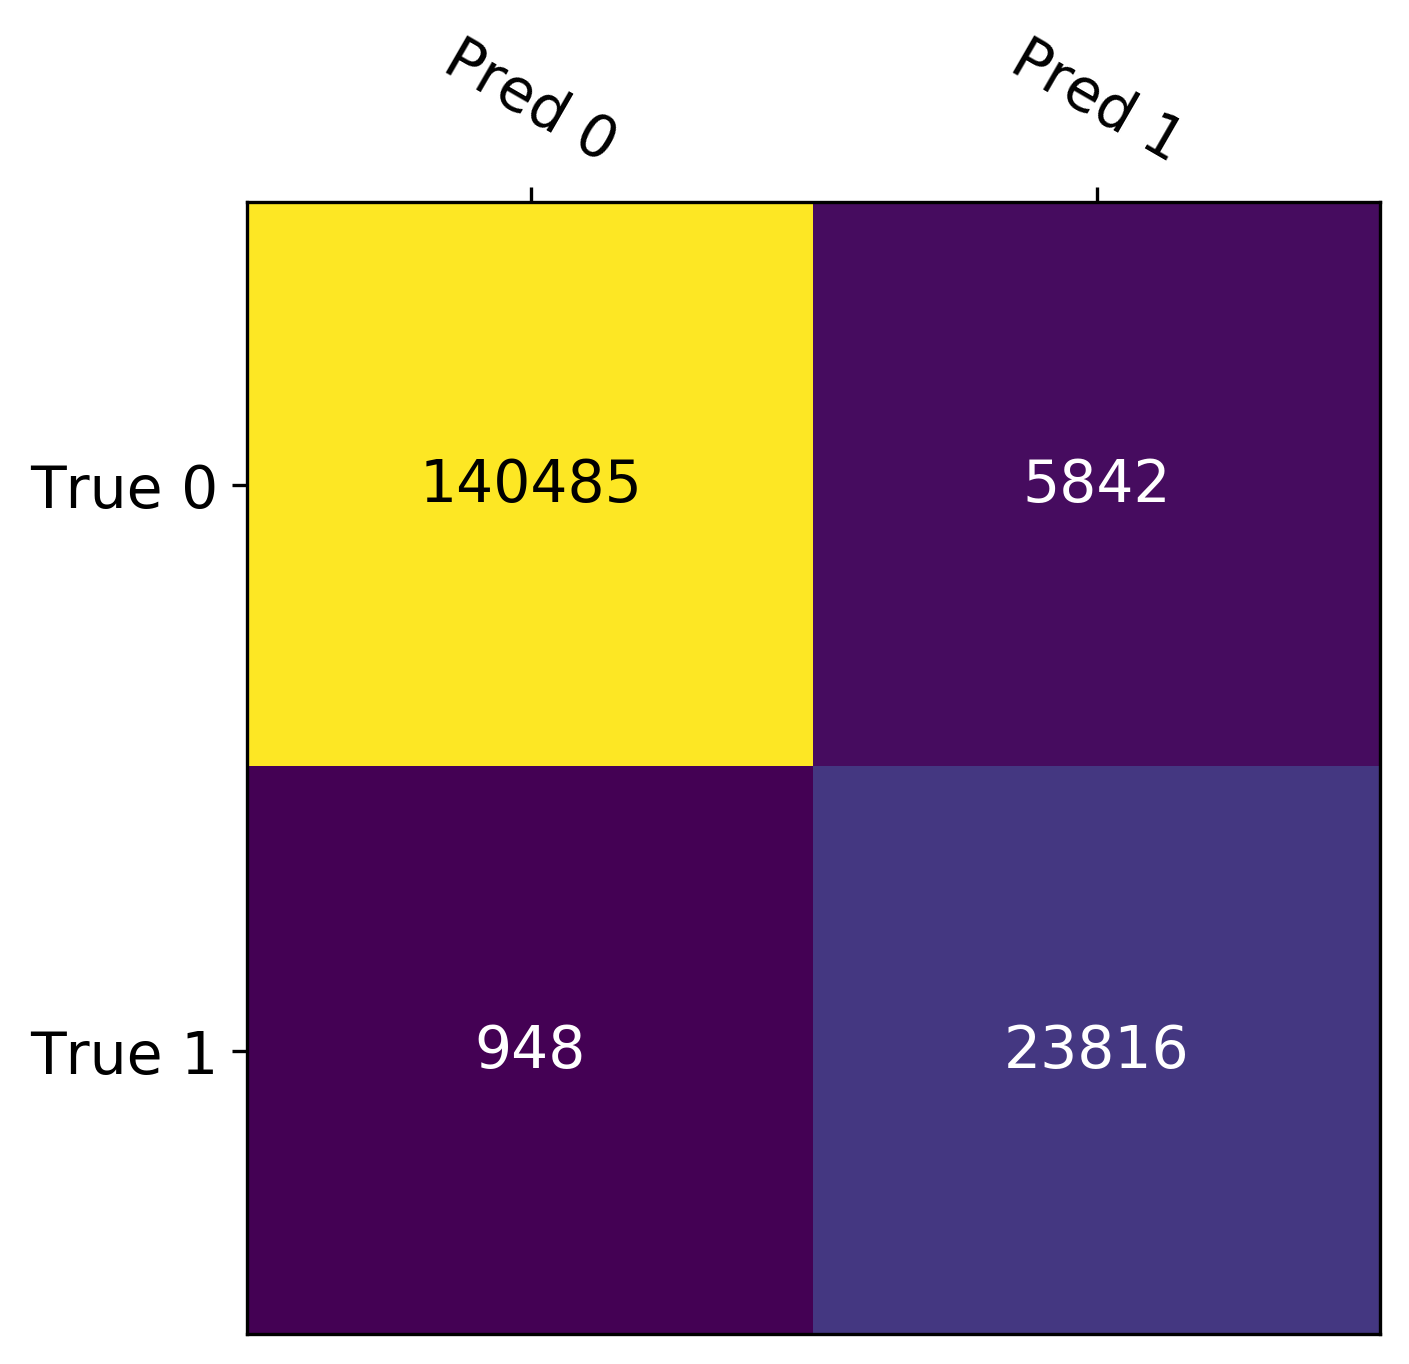
\includegraphics[height=3.75cm, valign=c]{assets/ind_cm_train}
    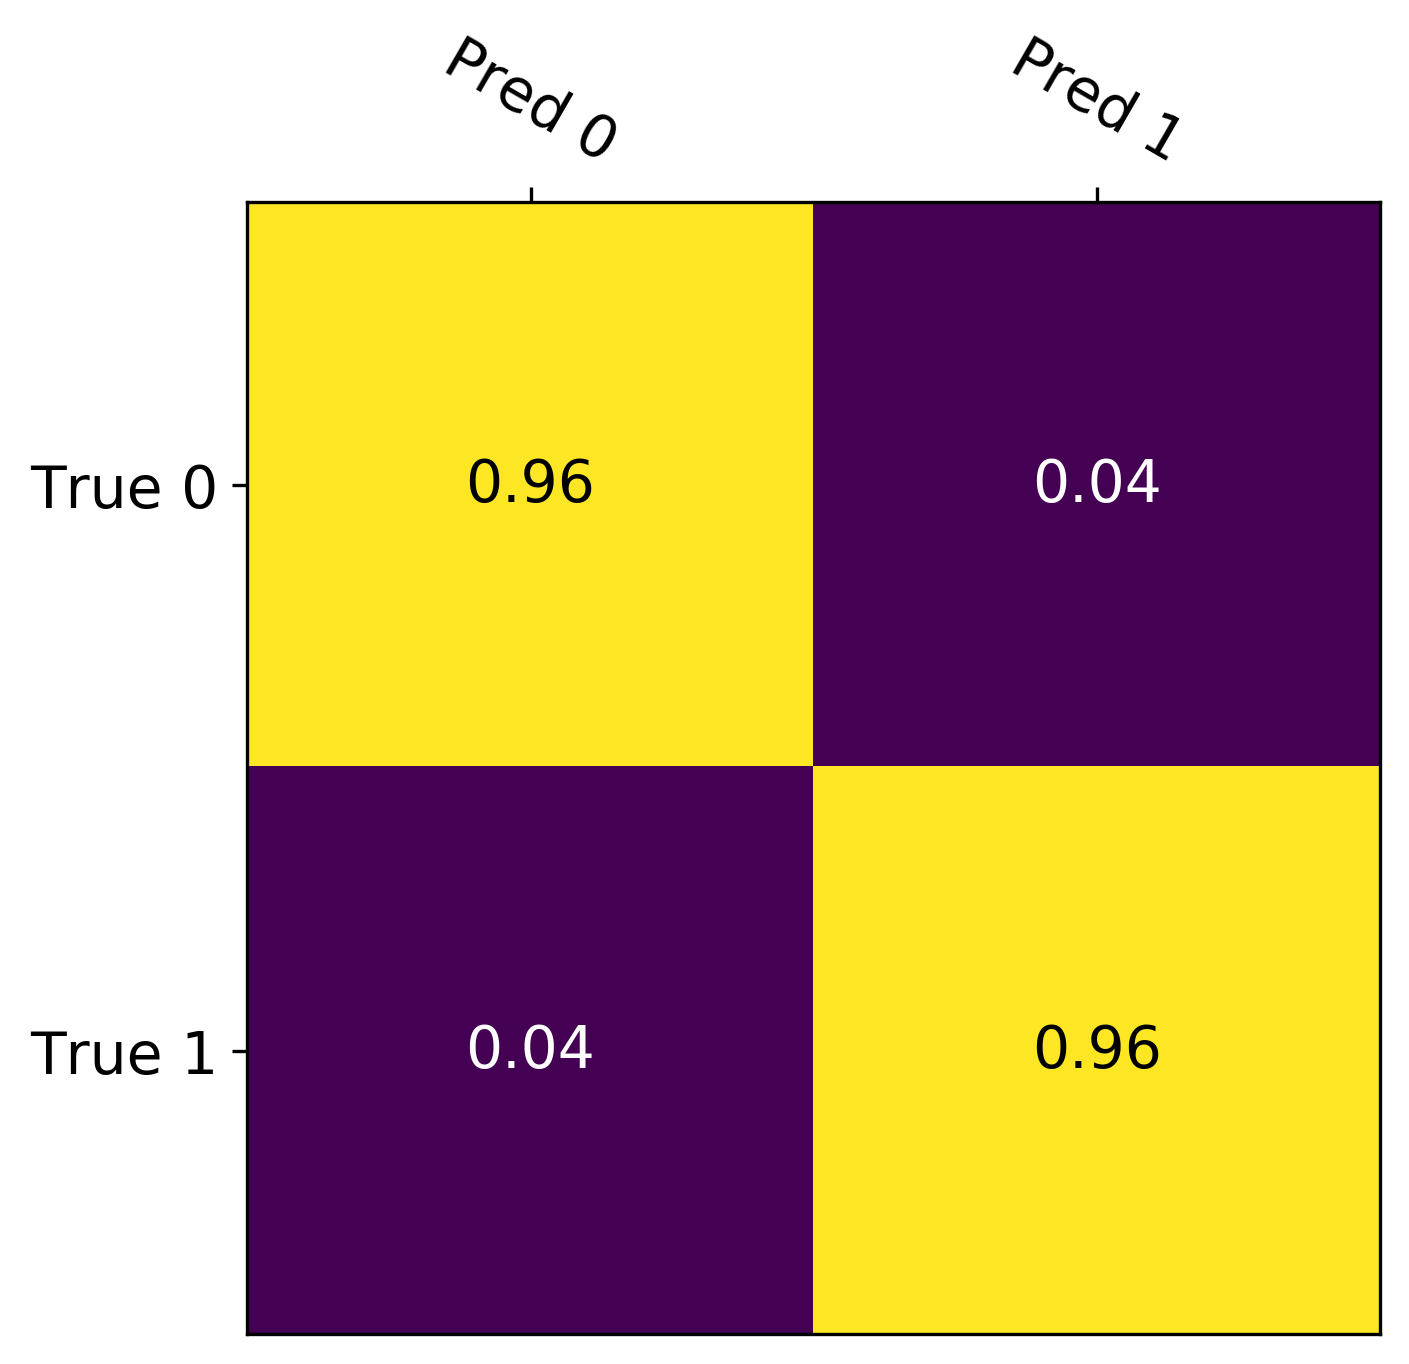
\includegraphics[height=3.75cm, valign=c]{assets/ind_cm_norm_train}
  \end{figure}
  \begin{center}
    \begin{tabular}{rcccr}
    \toprule
    {} &  Precision &  Recall &  F1-Score & Support \\
    \midrule
    Label: 0 & $0.99$ & $0.96$ & $0.98$ & $146,327$ \\
    Label: 1 & $0.80$ & $0.96$ & $0.88$ & $24,764$ \\
    \midrule
    accuracy & {} & {} & $0.96$ & $171,091$ \\
    macro avg & $0.90$ & $0.96$ & $0.93$ & $171,091$ \\
    weighted avg & $0.97$ & $0.96$ & $0.96$ & $171,091$ \\
    \bottomrule
    \end{tabular}
  \end{center}
  % something
  % metrics
  % graphs
\end{frame}

\begin{frame}
  \frametitle{Independent Row: Sample Results (Validation)}
  \begin{figure}
    \centering
    \includegraphics[height=3.75cm, valign=c]{assets/ind_cm_test}
    \includegraphics[height=3.75cm, valign=c]{assets/ind_cm_norm_test}
  \end{figure}
  \begin{center}
    \begin{tabular}{rcccr}
    \toprule
    {} &  Precision &  Recall &  F1-Score & Support \\
    \midrule
    Label: 0 & $0.97$ & $0.94$ & $0.95$ & $21,948$ \\
    Label: 1 & $0.71$ & $0.85$ & $0.77$ & $3,921$ \\
    \midrule
    accuracy & {} & {} & $0.92$ & $25,869$ \\
    macro avg & $0.84$ & $0.89$ & $0.86$ & $25,869$ \\
    weighted avg & $0.93$ & $0.92$ & $0.93$ & $25,869$ \\
    \bottomrule
    \end{tabular}
  \end{center}
  % something
  % metrics
  % graphs
\end{frame}

\begin{frame}
  \frametitle{How can we improve on this?}
  \begin{figure}
    \centering
    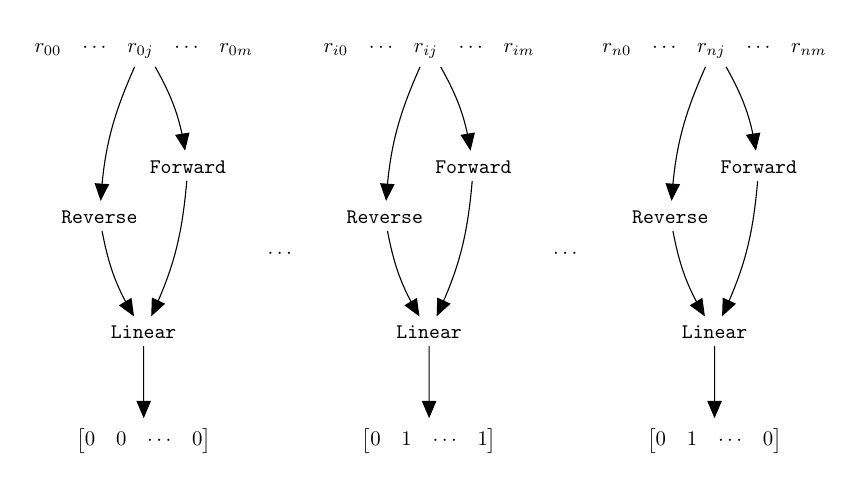
\begin{tikzpicture}[shorten >=1pt,node distance=1cm,on grid,auto, every node/.style={scale=0.75},
      el/.style={inner sep=2pt, align=left, sloped}]

      \node[] (r0) {$\begin{matrix} r_{00} & \cdots & r_{0j} & \cdots & r_{0m} \end{matrix}$};
      \node[] (for0) [below=of r0, yshift=-0.7cm, xshift=0.75cm] {$\texttt{Forward}$};
      \node[] (rev0) [below=of r0, yshift=-1.55cm, xshift=-0.75cm] {$\texttt{Reverse}$};

      \node[] (rnn1) [right=of r0, xshift=1cm, yshift=-3.5cm] {$\cdots$};

      \node[] (r1) [right=of r0, xshift=3.5cm] {$\begin{matrix} r_{i0} & \cdots & r_{ij} & \cdots & r_{im} \end{matrix}$};
      \node[] (for1) [below=of r1, yshift=-0.7cm, xshift=0.75cm] {$\texttt{Forward}$};
      \node[] (rev1) [below=of r1, yshift=-1.55cm, xshift=-0.75cm] {$\texttt{Reverse}$};

      \node[] (rnn2) [right=of r1, xshift=1cm, yshift=-3.5cm] {$\cdots$};

      \node[] (rn) [right=of r1, xshift=3.5cm] {$\begin{matrix} r_{n0} & \cdots & r_{nj} & \cdots & r_{nm} \end{matrix}$};
      \node[] (forn) [below=of rn, yshift=-0.7cm, xshift=0.75cm] {$\texttt{Forward}$};
      \node[] (revn) [below=of rn, yshift=-1.55cm, xshift=-0.75cm] {$\texttt{Reverse}$};

      \node[] (linear0) [below=of r0, yshift=-3.5cm] {$\texttt{Linear}$};
      \node[] (linear1) [below=of r1, yshift=-3.5cm] {$\texttt{Linear}$};
      \node[] (linearn) [below=of rn, yshift=-3.5cm] {$\texttt{Linear}$};

      \node[] (out0) [below=of linear0, yshift=-0.5cm] {$\begin{bmatrix} 0 & 0 & \cdots & 0 \end{bmatrix}$};
      \node[] (out1) [below=of linear1, yshift=-0.5cm] {$\begin{bmatrix} 0 & 1 & \cdots & 1 \end{bmatrix}$};
      \node[] (outn) [below=of linearn, yshift=-0.5cm] {$\begin{bmatrix} 0 & 1 & \cdots & 0 \end{bmatrix}$};

      \path[->]
        (r0) edge [bend left=10] node[] {} (for0)
        (r0) edge [bend right=10] node[] {} (rev0)
        (for0) edge [bend left=10] node[] {} (linear0)
        (rev0) edge [bend right=10] node[] {} (linear0)
        (linear0) edge [] node[] {} (out0)

        (r1) edge [bend left=10] node[] {} (for1)
        (r1) edge [bend right=10] node[] {} (rev1)
        (for1) edge [bend left=10] node[] {} (linear1)
        (rev1) edge [bend right=10] node[] {} (linear1)
        (linear1) edge [] node[] {} (out1)

        (rn) edge [bend left=10] node[] {} (forn)
        (rn) edge [bend right=10] node[] {} (revn)
        (forn) edge [bend left=10] node[] {} (linearn)
        (revn) edge [bend right=10] node[] {} (linearn)
        (linearn) edge [] node[] {} (outn);

    \end{tikzpicture}
  \end{figure}
\end{frame}

\begin{frame}
  \frametitle{Joint Training on a Table}
  \begin{itemize}
    \item We saw that we could regenerate a sequence from its hidden state alone.
    \item Why not use this information to link rows within the same table?
    \begin{itemize}
      \item Bidirectional for each row
      \item Propagate hidden state to next row
      \item Linear layers for prediction
    \end{itemize}
  \end{itemize}
  \begin{figure}
    \centering
    \includegraphics[width=10cm, valign=c]{assets/table_model}
  \end{figure}
\end{frame}

\begin{frame}
  \frametitle{Joint Table Training Visual}
  \begin{figure}
    \centering
    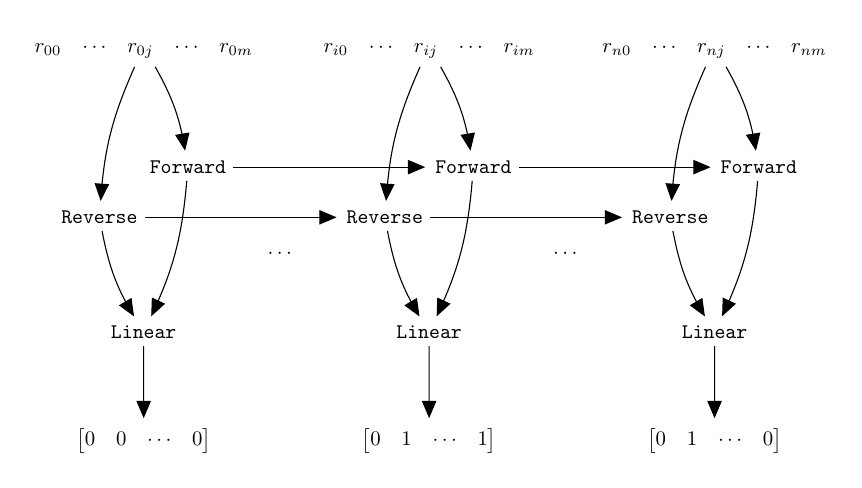
\begin{tikzpicture}[shorten >=1pt,node distance=1cm,on grid,auto, every node/.style={scale=0.75},
      el/.style={inner sep=2pt, align=left, sloped}]

      \node[] (r0) {$\begin{matrix} r_{00} & \cdots & r_{0j} & \cdots & r_{0m} \end{matrix}$};
      \node[] (for0) [below=of r0, yshift=-0.7cm, xshift=0.75cm] {$\texttt{Forward}$};
      \node[] (rev0) [below=of r0, yshift=-1.55cm, xshift=-0.75cm] {$\texttt{Reverse}$};

      \node[] (rnn1) [right=of r0, xshift=1cm, yshift=-3.5cm] {$\cdots$};

      \node[] (r1) [right=of r0, xshift=3.5cm] {$\begin{matrix} r_{i0} & \cdots & r_{ij} & \cdots & r_{im} \end{matrix}$};
      \node[] (for1) [below=of r1, yshift=-0.7cm, xshift=0.75cm] {$\texttt{Forward}$};
      \node[] (rev1) [below=of r1, yshift=-1.55cm, xshift=-0.75cm] {$\texttt{Reverse}$};

      \node[] (rnn2) [right=of r1, xshift=1cm, yshift=-3.5cm] {$\cdots$};

      \node[] (rn) [right=of r1, xshift=3.5cm] {$\begin{matrix} r_{n0} & \cdots & r_{nj} & \cdots & r_{nm} \end{matrix}$};
      \node[] (forn) [below=of rn, yshift=-0.7cm, xshift=0.75cm] {$\texttt{Forward}$};
      \node[] (revn) [below=of rn, yshift=-1.55cm, xshift=-0.75cm] {$\texttt{Reverse}$};

      \node[] (linear0) [below=of r0, yshift=-3.5cm] {$\texttt{Linear}$};
      \node[] (linear1) [below=of r1, yshift=-3.5cm] {$\texttt{Linear}$};
      \node[] (linearn) [below=of rn, yshift=-3.5cm] {$\texttt{Linear}$};

      \node[] (out0) [below=of linear0, yshift=-0.5cm] {$\begin{bmatrix} 0 & 0 & \cdots & 0 \end{bmatrix}$};
      \node[] (out1) [below=of linear1, yshift=-0.5cm] {$\begin{bmatrix} 0 & 1 & \cdots & 1 \end{bmatrix}$};
      \node[] (outn) [below=of linearn, yshift=-0.5cm] {$\begin{bmatrix} 0 & 1 & \cdots & 0 \end{bmatrix}$};


      \path[->]
        (r0) edge [bend left=10] node[] {} (for0)
        (r0) edge [bend right=10] node[] {} (rev0)
        (for0) edge [bend left=10] node[] {} (linear0)
        (rev0) edge [bend right=10] node[] {} (linear0)
        (linear0) edge [] node[] {} (out0)

        (r1) edge [bend left=10] node[] {} (for1)
        (r1) edge [bend right=10] node[] {} (rev1)
        (for1) edge [bend left=10] node[] {} (linear1)
        (rev1) edge [bend right=10] node[] {} (linear1)
        (linear1) edge [] node[] {} (out1)

        (rn) edge [bend left=10] node[] {} (forn)
        (rn) edge [bend right=10] node[] {} (revn)
        (forn) edge [bend left=10] node[] {} (linearn)
        (revn) edge [bend right=10] node[] {} (linearn)
        (linearn) edge [] node[] {} (outn)

        (for0) edge [] node[] {} (for1)
        (rev0) edge [] node[] {} (rev1)
        (for1) edge [] node[] {} (forn)
        (rev1) edge [] node[] {} (revn)
        ;


    \end{tikzpicture}
  \end{figure}
\end{frame}

\begin{frame}
  \frametitle{Joint Table Training: Sample Results (Training)}
  \begin{figure}
    \centering
    \includegraphics[height=3.75cm, valign=c]{assets/joint_cm_table_train}
    \includegraphics[height=3.75cm, valign=c]{assets/joint_cm_table_norm_train}
  \end{figure}
  \begin{center}
    \begin{tabular}{rcccr}
    \toprule
    {} &  Precision &  Recall &  F1-Score & Support \\
    \midrule
    Label: 0 & $1.00$ & $0.98$ & $0.99$ & $143,872$ \\
    Label: 1 & $0.88$ & $0.97$ & $0.93$ & $23,794$ \\
    \midrule
    accuracy & {} & {} & $0.98$ & $167,666$ \\
    macro avg & $0.94$ & $0.98$ & $0.96$ & $167,666$ \\
    weighted avg & $0.98$ & $0.98$ & $0.98$ & $167,666$ \\
    \bottomrule
    \end{tabular}
  \end{center}
  % something
  % metrics
  % graphs
\end{frame}

\begin{frame}
  \frametitle{Joint Table Training: Sample Results (Validation)}
  \begin{figure}
    \centering
    \includegraphics[height=3.75cm, valign=c]{assets/joint_cm_table_test}
    \includegraphics[height=3.75cm, valign=c]{assets/joint_cm_table_norm_test}
  \end{figure}
  \begin{center}
    \begin{tabular}{rcccr}
    \toprule
    {} &  Precision &  Recall &  F1-Score & Support \\
    \midrule
    Label: 0 & $0.97$ & $0.95$ & $0.96$ & $24,403$ \\
    Label: 1 & $0.78$ & $0.87$ & $0.82$ & $4,891$ \\
    \midrule
    accuracy & {} & {} & $0.94$ & $29,294$ \\
    macro avg & $0.88$ & $0.91$ & $0.89$ & $29,294$ \\
    weighted avg & $0.94$ & $0.94$ & $0.94$ & $29,294$ \\
    \bottomrule
    \end{tabular}
  \end{center}
  % something
  % metrics
  % graphs
\end{frame}

\begin{frame}
  \frametitle{Is this a correct way to link rows?}
  \begin{figure}
    \centering
    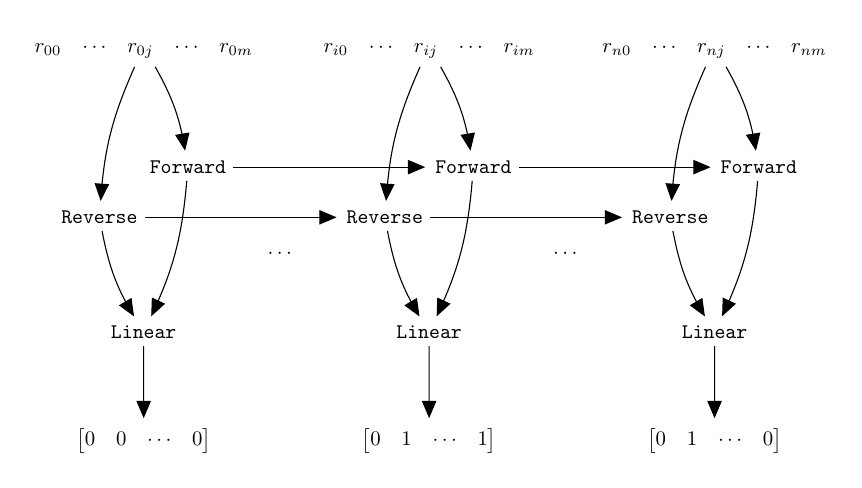
\begin{tikzpicture}[shorten >=1pt,node distance=1cm,on grid,auto, every node/.style={scale=0.75},
      el/.style={inner sep=2pt, align=left, sloped}]

      \node[] (r0) {$\begin{matrix} r_{00} & \cdots & r_{0j} & \cdots & r_{0m} \end{matrix}$};
      \node[] (for0) [below=of r0, yshift=-0.7cm, xshift=0.75cm] {$\texttt{Forward}$};
      \node[] (rev0) [below=of r0, yshift=-1.55cm, xshift=-0.75cm] {$\texttt{Reverse}$};

      \node[] (rnn1) [right=of r0, xshift=1cm, yshift=-3.5cm] {$\cdots$};

      \node[] (r1) [right=of r0, xshift=3.5cm] {$\begin{matrix} r_{i0} & \cdots & r_{ij} & \cdots & r_{im} \end{matrix}$};
      \node[] (for1) [below=of r1, yshift=-0.7cm, xshift=0.75cm] {$\texttt{Forward}$};
      \node[] (rev1) [below=of r1, yshift=-1.55cm, xshift=-0.75cm] {$\texttt{Reverse}$};

      \node[] (rnn2) [right=of r1, xshift=1cm, yshift=-3.5cm] {$\cdots$};

      \node[] (rn) [right=of r1, xshift=3.5cm] {$\begin{matrix} r_{n0} & \cdots & r_{nj} & \cdots & r_{nm} \end{matrix}$};
      \node[] (forn) [below=of rn, yshift=-0.7cm, xshift=0.75cm] {$\texttt{Forward}$};
      \node[] (revn) [below=of rn, yshift=-1.55cm, xshift=-0.75cm] {$\texttt{Reverse}$};

      \node[] (linear0) [below=of r0, yshift=-3.5cm] {$\texttt{Linear}$};
      \node[] (linear1) [below=of r1, yshift=-3.5cm] {$\texttt{Linear}$};
      \node[] (linearn) [below=of rn, yshift=-3.5cm] {$\texttt{Linear}$};

      \node[] (out0) [below=of linear0, yshift=-0.5cm] {$\begin{bmatrix} 0 & 0 & \cdots & 0 \end{bmatrix}$};
      \node[] (out1) [below=of linear1, yshift=-0.5cm] {$\begin{bmatrix} 0 & 1 & \cdots & 1 \end{bmatrix}$};
      \node[] (outn) [below=of linearn, yshift=-0.5cm] {$\begin{bmatrix} 0 & 1 & \cdots & 0 \end{bmatrix}$};


      \path[->]
        (r0) edge [bend left=10] node[] {} (for0)
        (r0) edge [bend right=10] node[] {} (rev0)
        (for0) edge [bend left=10] node[] {} (linear0)
        (rev0) edge [bend right=10] node[] {} (linear0)
        (linear0) edge [] node[] {} (out0)

        (r1) edge [bend left=10] node[] {} (for1)
        (r1) edge [bend right=10] node[] {} (rev1)
        (for1) edge [bend left=10] node[] {} (linear1)
        (rev1) edge [bend right=10] node[] {} (linear1)
        (linear1) edge [] node[] {} (out1)

        (rn) edge [bend left=10] node[] {} (forn)
        (rn) edge [bend right=10] node[] {} (revn)
        (forn) edge [bend left=10] node[] {} (linearn)
        (revn) edge [bend right=10] node[] {} (linearn)
        (linearn) edge [] node[] {} (outn)

        (for0) edge [] node[] {} (for1)
        (rev0) edge [] node[] {} (rev1)
        (for1) edge [] node[] {} (forn)
        (rev1) edge [] node[] {} (revn)
        ;


    \end{tikzpicture}
  \end{figure}
\end{frame}

\begin{frame}
  \frametitle{Joint Table Training with Swapping Visual}
  \begin{figure}
    \centering
    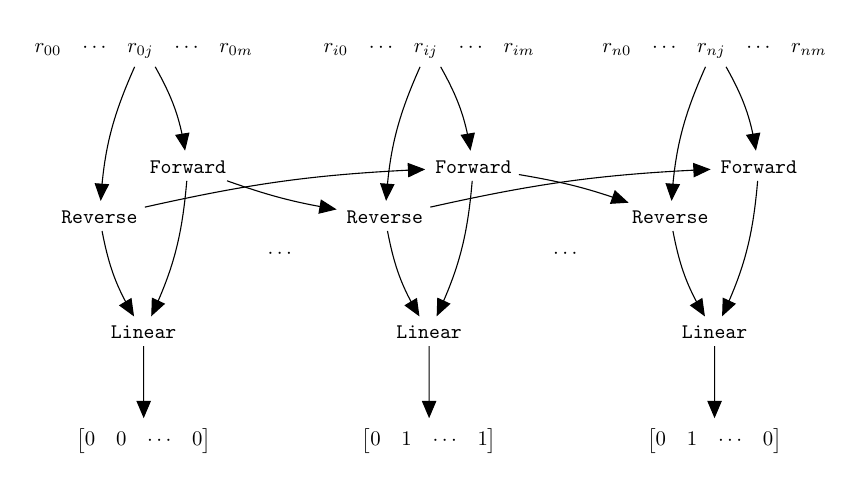
\begin{tikzpicture}[shorten >=1pt,node distance=1cm,on grid,auto, every node/.style={scale=0.75},
      el/.style={inner sep=2pt, align=left, sloped}]

      \node[] (r0) {$\begin{matrix} r_{00} & \cdots & r_{0j} & \cdots & r_{0m} \end{matrix}$};
      \node[] (for0) [below=of r0, yshift=-0.7cm, xshift=0.75cm] {$\texttt{Forward}$};
      \node[] (rev0) [below=of r0, yshift=-1.55cm, xshift=-0.75cm] {$\texttt{Reverse}$};

      \node[] (rnn1) [right=of r0, xshift=1cm, yshift=-3.5cm] {$\cdots$};

      \node[] (r1) [right=of r0, xshift=3.5cm] {$\begin{matrix} r_{i0} & \cdots & r_{ij} & \cdots & r_{im} \end{matrix}$};
      \node[] (for1) [below=of r1, yshift=-0.7cm, xshift=0.75cm] {$\texttt{Forward}$};
      \node[] (rev1) [below=of r1, yshift=-1.55cm, xshift=-0.75cm] {$\texttt{Reverse}$};

      \node[] (rnn2) [right=of r1, xshift=1cm, yshift=-3.5cm] {$\cdots$};

      \node[] (rn) [right=of r1, xshift=3.5cm] {$\begin{matrix} r_{n0} & \cdots & r_{nj} & \cdots & r_{nm} \end{matrix}$};
      \node[] (forn) [below=of rn, yshift=-0.7cm, xshift=0.75cm] {$\texttt{Forward}$};
      \node[] (revn) [below=of rn, yshift=-1.55cm, xshift=-0.75cm] {$\texttt{Reverse}$};

      \node[] (linear0) [below=of r0, yshift=-3.5cm] {$\texttt{Linear}$};
      \node[] (linear1) [below=of r1, yshift=-3.5cm] {$\texttt{Linear}$};
      \node[] (linearn) [below=of rn, yshift=-3.5cm] {$\texttt{Linear}$};

      \node[] (out0) [below=of linear0, yshift=-0.5cm] {$\begin{bmatrix} 0 & 0 & \cdots & 0 \end{bmatrix}$};
      \node[] (out1) [below=of linear1, yshift=-0.5cm] {$\begin{bmatrix} 0 & 1 & \cdots & 1 \end{bmatrix}$};
      \node[] (outn) [below=of linearn, yshift=-0.5cm] {$\begin{bmatrix} 0 & 1 & \cdots & 0 \end{bmatrix}$};


      \path[->]
        (r0) edge [bend left=10] node[] {} (for0)
        (r0) edge [bend right=10] node[] {} (rev0)
        (for0) edge [bend left=10] node[] {} (linear0)
        (rev0) edge [bend right=10] node[] {} (linear0)
        (linear0) edge [] node[] {} (out0)

        (r1) edge [bend left=10] node[] {} (for1)
        (r1) edge [bend right=10] node[] {} (rev1)
        (for1) edge [bend left=10] node[] {} (linear1)
        (rev1) edge [bend right=10] node[] {} (linear1)
        (linear1) edge [] node[] {} (out1)

        (rn) edge [bend left=10] node[] {} (forn)
        (rn) edge [bend right=10] node[] {} (revn)
        (forn) edge [bend left=10] node[] {} (linearn)
        (revn) edge [bend right=10] node[] {} (linearn)
        (linearn) edge [] node[] {} (outn)

        (for0) edge [bend right=5] node[] {} (rev1)
        (rev0) edge [bend left=5] node[] {} (for1)
        (for1) edge [bend left=5] node[] {} (revn)
        (rev1) edge [bend left=5] node[] {} (forn)
        ;


    \end{tikzpicture}
  \end{figure}
\end{frame}


\begin{frame}
  \frametitle{Trick for Swapping in Joint Table Training}
  \begin{itemize}
    \item Note that the hidden state is biased towards the items closest to it
    \item So the beginning of a new row has context from the end of the last row
    \begin{itemize}
      \item Is this a good choice?
      \item What if we flip the bidirectional hidden states every iteration
      \item AKA the beginning of a new row has the hidden state info from the beginning of the last row
      \item And vice-versa
    \end{itemize}
  \end{itemize}
  \begin{figure}
    \centering
    \includegraphics[width=10cm, valign=c]{assets/table_model_swap}
  \end{figure}
\end{frame}

\begin{frame}
  \frametitle{Joint Table Training with Swapping: Sample Results (Training)}
  \begin{figure}
    \centering
    \includegraphics[height=3.75cm, valign=c]{assets/swap_cm_table_train}
    \includegraphics[height=3.75cm, valign=c]{assets/swap_cm_table_norm_train}
  \end{figure}
  \begin{center}
    \begin{tabular}{rcccr}
    \toprule
    {} &  Precision &  Recall &  F1-Score & Support \\
    \midrule
    Label: 0 & $0.99$ & $0.98$ & $0.99$ & $143,872$ \\
    Label: 1 & $0.88$ & $0.96$ & $0.91$ & $23,794$ \\
    \midrule
    accuracy & {} & {} & $0.97$ & $167,666$ \\
    macro avg & $0.93$ & $0.97$ & $0.95$ & $167,666$ \\
    weighted avg & $0.98$ & $0.97$ & $0.98$ & $167,666$ \\
    \bottomrule
    \end{tabular}
  \end{center}
  % something
  % metrics
  % graphs
\end{frame}

\begin{frame}
  \frametitle{Joint Table Training with Swapping: Sample Results (Validation)}
  \begin{figure}
    \centering
    \includegraphics[height=3.75cm, valign=c]{assets/swap_cm_table_test}
    \includegraphics[height=3.75cm, valign=c]{assets/swap_cm_table_norm_test}
  \end{figure}
  \begin{center}
    \begin{tabular}{rcccr}
    \toprule
    {} &  Precision &  Recall &  F1-Score & Support \\
    \midrule
    Label: 0 & $0.97$ & $0.95$ & $0.96$ & $24,403$ \\
    Label: 1 & $0.78$ & $0.83$ & $0.80$ & $4,891$ \\
    \midrule
    accuracy & {} & {} & $0.93$ & $29,294$ \\
    macro avg & $0.87$ & $0.89$ & $0.88$ & $29,294$ \\
    weighted avg & $0.93$ & $0.93$ & $0.93$ & $29,294$ \\
    \bottomrule
    \end{tabular}
  \end{center}
  % something
  % metrics
  % graphs
\end{frame}

\begin{frame}
  \frametitle{Summary of Methods (Validation)}
  \begin{center}
    \footnotesize
    % \begin{tabular}{rccc|ccc|c}
    % \toprule
    % {} & \multicolumn{3}{c}{Label 0} & \multicolumn{3}{c}{Label 1} & {} \\
    % \cmidrule(lr){1-4}  \cmidrule(lr){5-7}
    % {} &  Precision &  Recall &  F1-Score & Precision &  Recall &  F1-Score & Accuracy \\
    % \midrule
    % Independent   & $0.99$ & $0.92$ & $0.96$ & $0.67$ & $0.97$ & $0.80$ & $0.93$ \\
    % Joint Table   & $1.00$ & $0.96$ & $0.98$ & $0.83$ & $0.98$ & $0.90$ & $0.97$ \\
    % Joint Swapped & $1.00$ & $0.97$ & $0.98$ & $0.83$ & $0.98$ & $0.90$ & $0.97$ \\
    % \bottomrule
    % \end{tabular}

    \begin{tabular}{rlccc}
    \toprule
    {} & {} & Independent & Joint & Joint Swapped \\
    \midrule
    \multirow{3}{*}{Label: 0} & Precision & $\mathbf{0.97}$ & $\mathbf{0.97}$ & $\mathbf{0.97}$ \\
    {}                        & Recall    & $0.94$ & $\mathbf{0.95}$ & $\mathbf{0.95}$ \\
    {}                        & F1-Score  & $0.95$ & $\mathbf{0.96}$ & $\mathbf{0.96}$ \\
    \midrule
    \multirow{3}{*}{Label: 1} & Precision & $0.71$ & $\mathbf{0.78}$ & $\mathbf{0.78}$ \\
    {}                        & Recall    & $0.85$ & $\mathbf{0.87}$ & $0.83$ \\
    {}                        & F1-Score  & $0.77$ & $\mathbf{0.82}$ & $0.80$ \\
    \midrule
    {}                        & Accuracy  & $0.92$ & $\mathbf{0.94}$ & $0.93$ \\
    \bottomrule
    \end{tabular}
  \end{center}
\end{frame}

\begin{frame}
  \frametitle{What have we learned?}
  \begin{itemize}
    \item We can learn text segments purely from the sequence of Part-of-Speech tags
    \item It is useful to jointly train/predict on the table instead of assuming independence
    \item Is there any benefit to swapping hidden states during propagation?
    \item \textbf{Note:}
    \begin{itemize}
      \item We use the concept of \textit{deep transition} in Seq2Seq for joint training
      \item Where our training is dependent on the hidden state encoding useful information
    \end{itemize}
  \end{itemize}
\end{frame}


\begin{frame}
  \frametitle{Future Plans}
  \begin{itemize}
    \item Features
    \begin{itemize}
      \item Use word location information
      \item Tesseract gives bounding boxes
    \end{itemize}
    \item Encoder Structure
    \begin{itemize}
      \item Convolution
      \item Transformer
    \end{itemize}
  \end{itemize}
\end{frame}


%%%%%%%%%%%%%%%%%%%%%%%%%%%%%%%%%%%%%%%%%%%%%%%%%%%%%%%%%%%%%%%%%%%%%%%%%%%%%%%%

\section{Other Applications For Sequence Modeling}

\begin{frame}
\frametitle{Recall: Encoders, Decoders, and Seq2Seq Models}
\begin{itemize}
  \item \textbf{Encoders} given a sequence meaning
  \item \textbf{Decoders} generate a new sequence
  \item \textbf{Seq2Seq} generate sequences conditioned on another sequence
\end{itemize}
\end{frame}

\begin{frame}
  \frametitle{What to use for which application?}
  \begin{itemize}
    \item \textbf{Encoders}
    \begin{itemize}
      \item POS Tagging
      \item Sentence Embeddings
      \item Anything where you are given the sentence at test time
    \end{itemize}
    \item \textbf{Decoders}
    \begin{itemize}
      \item Text Generation
      \item Language Modeling
      \item Anything where you need to create a sequence at test time
    \end{itemize}
    \item \textbf{Seq2Seq}
      \begin{itemize}
        \item Translation
        \item Speech Recognition
        \item Summarization
        \item Question/Answering
        \item Anything where you convert a sequence into another sequence
      \end{itemize}
  \end{itemize}
\end{frame}

%%%%%%%%%%%%%%%%%%%%%%%%%%%%%%%%%%%%%%%%%%%%%%%%%%%%%%%%%%%%%%%%%%%%%%%%%%%%%%%%

\section{Tools, References, and Further Reading}

\begin{frame}
  \frametitle{Acknowledgment}
  \begin{itemize}
    \item Pieces adapted from my \href{http://mt-class.org/jhu/}{college Machine Translation Course by Philipp Koehn}
    \item Additional acknowledgment:
    \begin{itemize}
      \item \href{http://alopez.github.io/}{Adam Lopez}
      \item \href{http://www.cs.jhu.edu/~post/}{Matt Post}
      \item \href{http://www.cis.upenn.edu/~ccb/}{Chris Callison-Burch}
      \item \href{http://www.cs.jhu.edu/~phi/}{Philipp Koehn}
    \end{itemize}
  \end{itemize}
\end{frame}

\begin{frame}
  \frametitle{Papers}
  \begin{itemize}
    \item \href{https://arxiv.org/abs/1409.3215}{Sutskever et al., Sequence to Sequence Learning with Neural Networks}
    \item \href{https://arxiv.org/abs/1406.1078}{Cho et al., Learning Phrase Representations using RNN Encoder-Decoder for Statistical Machine Translation}
    \item \href{https://arxiv.org/pdf/1508.07909}{Sennrich et al., Neural Machine Translation of Rare Words with Subword Units}
    \item \href{https://arxiv.org/abs/1709.07809}{Koehn, Neural Machine Translation}
    \item \href{https://www.aclweb.org/anthology/W17-3204.pdf}{Koehn, Six Challenges for Neural Machine Translation}
    \item \href{https://github.com/THUNLP-MT/MT-Reading-List}{Curated Machine Translation Reading List}
  \end{itemize}
\end{frame}

\begin{frame}
  \frametitle{Tutorials}
  \begin{itemize}
    \item Pytorch
    \begin{itemize}
      \item \href{https://pytorch.org/tutorials/intermediate/seq2seq_translation_tutorial.html}{Official PyTorch Seq2Seq Tutorial}
      \item \href{https://pytorch.org/tutorials/beginner/torchtext_translation_tutorial.html}{PyTorch Seq2Seq with Torchtext}
      \item \href{https://github.com/bentrevett/pytorch-seq2seq}{Ben Trevett Seq2Seq Tutorial}
    \end{itemize}
    \item Tensorflow
    \begin{itemize}
      \item \href{https://www.tensorflow.org/tutorials/text/nmt_with_attention}{NMT with Attention}
    \end{itemize}
  \end{itemize}
\end{frame}

\begin{frame}
\frametitle{Libraries}
  \begin{itemize}
    \item \href{https://github.com/pytorch/fairseq}{Facebook: fairseq (PyTorch)}
    \item \href{https://github.com/OpenNMT/OpenNMT-py}{Open NMT (PyTorch)}
    \item \href{https://github.com/OpenNMT/OpenNMT-tf}{Open NMT (Tensorflow)}
  \end{itemize}
\end{frame}

\section{Thank You!}


% Refs, ideas, etc


\end{document}
